\chapter{Mapped classification data for each patient} \label{MappedClassificationData}

\newgeometry{bottom=4cm} %set the left margin of page
\begin{landscape}
\begin{figure}[htbp]
\begin{subfigure}{6.5cm}
    \makebox[60pt]{\raisebox{50pt}{\rotatebox[origin=c]{0}{\minibox{IPF2 Classified\\ data}}}}%
    \sbox0{\includegraphics{Appendix/Image_AppexC/IPF2_ClassifiedData_Time1.png}}% get image width, trim={<left> <lower> <right> <upper>}
    \begin{overpic}[height=1.65in,trim={{.0\wd0} {.0\wd0} {.0\wd0} {.0\wd0}},clip]{Appendix/Image_AppexC/IPF2_ClassifiedData_Time1.png}
    \end{overpic}
    \makebox[60pt]{\raisebox{60pt}{\rotatebox[origin=c]{0}{\minibox{IPF2 Mapped\\ data}}}}% \makebox:change left space, \raisebox: change upper space
    \begin{overpic}[height=1.6in,trim={{.0\wd0} {.0\wd0} {.0\wd0} {.0\wd0}},clip]{Appendix/Image_AppexC/IPF2_MappedData_Time1.png}
    \end{overpic}
    \caption{Time point 1}
		\label{fig:IPF2MappingResult-a}
\end{subfigure}\hspace{0.3cm}
\begin{subfigure}{4.8cm}
    \sbox0{\includegraphics{Appendix/Image_AppexC/IPF2_ClassifiedData_Time2.png}}% get image width, trim={<left> <lower> <right> <upper>}
    \begin{overpic}[height=1.62in,trim={{.0\wd0} {.0\wd0} {.0\wd0} {.0\wd0}},clip]{Appendix/Image_AppexC/IPF2_ClassifiedData_Time2.png}
    \end{overpic}
    \begin{overpic}[height=1.63in,trim={{.0\wd0} {.0\wd0} {.0\wd0} {.0\wd0}},clip]{Appendix/Image_AppexC/IPF2_MappedData_Time2.png}
    \end{overpic}
    \caption{Time point 2}
		\label{fig:IPF2MappingResult-b}
\end{subfigure}\hspace{0.3cm}
\begin{subfigure}{4.8cm}
    \sbox0{\includegraphics{Appendix/Image_AppexC/IPF2_ClassifiedData_Time3.png}}% get image width, trim={<left> <lower> <right> <upper>}
    \begin{overpic}[height=1.59in,trim={{.0\wd0} {.0\wd0} {.0\wd0} {.0\wd0}},clip]{Appendix/Image_AppexC/IPF2_ClassifiedData_Time3.png}
    \end{overpic}
    \begin{overpic}[height=1.62in,trim={{.0\wd0} {.0\wd0} {.0\wd0} {.0\wd0}},clip]{Appendix/Image_AppexC/IPF2_MappedData_Time3.png}
    \end{overpic}
    \caption{Time point 3}
		\label{fig:IPF2MappingResult-c}
\end{subfigure}
\begin{subfigure}{2cm}
    \makebox[30pt]{\raisebox{100pt}{\rotatebox[origin=c]{0}{\minibox{\\}}}}
    \sbox0{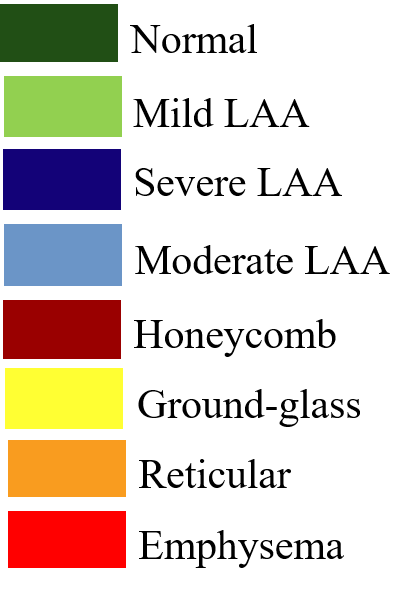
\includegraphics{Appendix/Image_AppexC/ClassifiedColor_new.png}}% get image width, trim={<left> <lower> <right> <upper>}
    \begin{overpic}[height=1.78in,trim={{.0\wd0} {.0\wd0} {.0\wd0} {.0\wd0}},clip]{Appendix/Image_AppexC/ClassifiedColor_new.png}
    \end{overpic}
\end{subfigure}
\caption{Classified data (top row) and mapped data (bottom row) of three time points of case IPF2. (a) The first time point, scan time: 0 month. (b) The second time point, scan time: 15 months. (c) The third time point, scan time: 35 months}
\label{fig:IPF2MappingResult}
\end{figure}
\end{landscape}
\restoregeometry

\newgeometry{bottom=4cm} %set the left margin of page
\begin{landscape}
\begin{figure}[htbp]
\begin{subfigure}{6.5cm}
    \makebox[60pt]{\raisebox{50pt}{\rotatebox[origin=c]{0}{\minibox{IPF3 Classified\\ data}}}}%
    \sbox0{\includegraphics{Appendix/Image_AppexC/IPF3_ClassifiedData_Time1.png}}% get image width, trim={<left> <lower> <right> <upper>}
    \begin{overpic}[height=1.62in,trim={{.0\wd0} {.0\wd0} {.0\wd0} {.0\wd0}},clip]{Appendix/Image_AppexC/IPF3_ClassifiedData_Time1.png}
    \end{overpic}
    \makebox[60pt]{\raisebox{60pt}{\rotatebox[origin=c]{0}{\minibox{IPF3 Mapped\\ data}}}}% \makebox:change left space, \raisebox: change upper space
    \begin{overpic}[height=1.6in,trim={{.0\wd0} {.0\wd0} {.0\wd0} {.0\wd0}},clip]{Appendix/Image_AppexC/IPF3_MappedData_Time1.png}
    \end{overpic}
    \caption{Time point 1}
		\label{fig:IPF3MappingResult-a}
\end{subfigure}\hspace{0.3cm}
\begin{subfigure}{4.8cm}
    \sbox0{\includegraphics{Appendix/Image_AppexC/IPF3_ClassifiedData_Time2.png}}% get image width, trim={<left> <lower> <right> <upper>}
    \begin{overpic}[height=1.59in,trim={{.0\wd0} {.0\wd0} {.0\wd0} {.0\wd0}},clip]{Appendix/Image_AppexC/IPF3_ClassifiedData_Time2.png}
    \end{overpic}
    \begin{overpic}[height=1.63in,trim={{.0\wd0} {.0\wd0} {.0\wd0} {.0\wd0}},clip]{Appendix/Image_AppexC/IPF3_MappedData_Time2.png}
    \end{overpic}
    \caption{Time point 2}
		\label{fig:IPF3MappingResult-b}
\end{subfigure}\hspace{0.3cm}
\begin{subfigure}{4.8cm}
    \sbox0{\includegraphics{Appendix/Image_AppexC/IPF3_ClassifiedData_Time3.png}}% get image width, trim={<left> <lower> <right> <upper>}
    \begin{overpic}[height=1.56in,trim={{.0\wd0} {.0\wd0} {.0\wd0} {.0\wd0}},clip]{Appendix/Image_AppexC/IPF3_ClassifiedData_Time3.png}
    \end{overpic}
    \begin{overpic}[height=1.62in,trim={{.0\wd0} {.0\wd0} {.0\wd0} {.0\wd0}},clip]{Appendix/Image_AppexC/IPF3_MappedData_Time3.png}
    \end{overpic}
    \caption{Time point 3}
		\label{fig:IPF3MappingResult-c}
\end{subfigure}
\begin{subfigure}{2cm}
    \makebox[30pt]{\raisebox{100pt}{\rotatebox[origin=c]{0}{\minibox{\\}}}}
    \sbox0{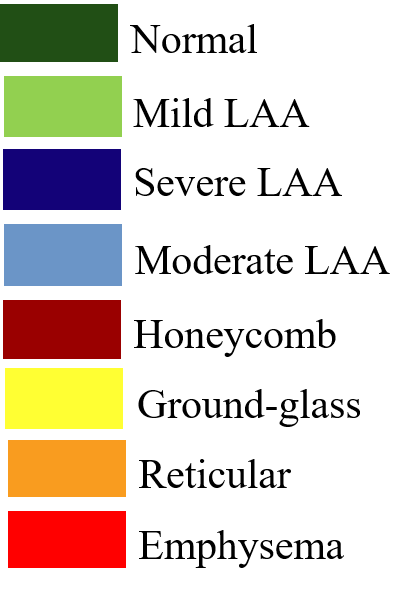
\includegraphics{Appendix/Image_AppexC/ClassifiedColor_new.png}}% get image width, trim={<left> <lower> <right> <upper>}
    \begin{overpic}[height=1.78in,trim={{.0\wd0} {.0\wd0} {.0\wd0} {.0\wd0}},clip]{Appendix/Image_AppexC/ClassifiedColor_new.png}
    \end{overpic}
\end{subfigure}
\caption{Classified data (top row) and mapped data (bottom row) of three time points of case IPF3. (a) The first time point, scan time: 0 month. (b) The second time point, scan time: 11 months. (c) The third time point, scan time: 30 months}
\label{fig:IPF3MappingResult}
\end{figure}
\end{landscape}
\restoregeometry

\newgeometry{bottom=4cm} %set the left margin of page
\begin{landscape}
\begin{figure}[htbp]
\begin{subfigure}{6.5cm}
    \makebox[60pt]{\raisebox{50pt}{\rotatebox[origin=c]{0}{\minibox{IPF5 Classified\\ data}}}}%
    \sbox0{\includegraphics{Appendix/Image_AppexC/IPF5_ClassifiedData_Time1.png}}% get image width, trim={<left> <lower> <right> <upper>}
    \begin{overpic}[height=1.65in,trim={{.0\wd0} {.0\wd0} {.0\wd0} {.0\wd0}},clip]{Appendix/Image_AppexC/IPF5_ClassifiedData_Time1.png}
    \end{overpic}
    \makebox[60pt]{\raisebox{60pt}{\rotatebox[origin=c]{0}{\minibox{IPF5 Mapped\\ data}}}}% \makebox:change left space, \raisebox: change upper space
    \begin{overpic}[height=1.65in,trim={{.0\wd0} {.0\wd0} {.0\wd0} {.0\wd0}},clip]{Appendix/Image_AppexC/IPF5_MappedData_Time1.png}
    \end{overpic}
    \caption{Time point 1}
		\label{fig:IPF5MappingResult-a}
\end{subfigure}\hspace{0.3cm}
\begin{subfigure}{4.8cm}
    \sbox0{\includegraphics{Appendix/Image_AppexC/IPF5_ClassifiedData_Time2.png}}% get image width, trim={<left> <lower> <right> <upper>}
    \begin{overpic}[height=1.62in,trim={{.0\wd0} {.0\wd0} {.0\wd0} {.0\wd0}},clip]{Appendix/Image_AppexC/IPF5_ClassifiedData_Time2.png}
    \end{overpic}
    \begin{overpic}[height=1.66in,trim={{.0\wd0} {.0\wd0} {.0\wd0} {.0\wd0}},clip]{Appendix/Image_AppexC/IPF5_MappedData_Time2.png}
    \end{overpic}
    \caption{Time point 2}
		\label{fig:IPF5MappingResult-b}
\end{subfigure}\hspace{0.3cm}
\begin{subfigure}{4.8cm}
    \sbox0{\includegraphics{Appendix/Image_AppexC/IPF5_ClassifiedData_Time3.png}}% get image width, trim={<left> <lower> <right> <upper>}
    \begin{overpic}[height=1.59in,trim={{.0\wd0} {.0\wd0} {.0\wd0} {.0\wd0}},clip]{Appendix/Image_AppexC/IPF5_ClassifiedData_Time3.png}
    \end{overpic}
    \begin{overpic}[height=1.65in,trim={{.0\wd0} {.0\wd0} {.0\wd0} {.0\wd0}},clip]{Appendix/Image_AppexC/IPF5_MappedData_Time3.png}
    \end{overpic}
    \caption{Time point 3}
		\label{fig:IPF5MappingResult-c}
\end{subfigure}
\begin{subfigure}{2cm}
    \makebox[30pt]{\raisebox{100pt}{\rotatebox[origin=c]{0}{\minibox{\\}}}}
    \sbox0{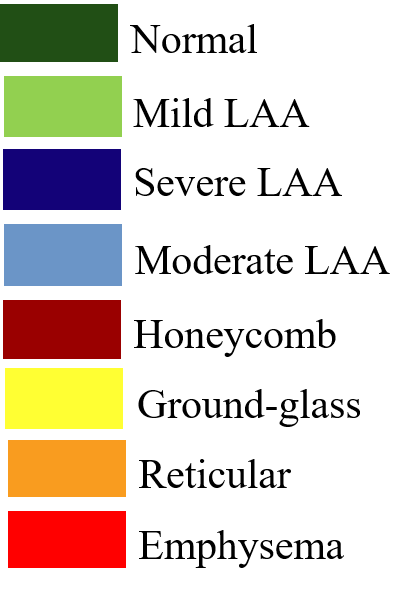
\includegraphics{Appendix/Image_AppexC/ClassifiedColor_new.png}}% get image width, trim={<left> <lower> <right> <upper>}
    \begin{overpic}[height=1.78in,trim={{.0\wd0} {.0\wd0} {.0\wd0} {.0\wd0}},clip]{Appendix/Image_AppexC/ClassifiedColor_new.png}
    \end{overpic}
\end{subfigure}
\caption{Classified data (top row) and mapped data (bottom row) of three time points of case IPF5. (a) The first time point, scan time: 0 month. (b) The second time point, scan time: 12 months. (c) The third time point, scan time: 23 months}
\label{fig:IPF5MappingResult}
\end{figure}
\end{landscape}
\restoregeometry

\newgeometry{bottom=4cm} %set the left margin of page
\begin{landscape}
\begin{figure}[htbp]
\begin{subfigure}{6.5cm}
    \makebox[60pt]{\raisebox{50pt}{\rotatebox[origin=c]{0}{\minibox{IPF6 Classified\\ data}}}}%
    \sbox0{\includegraphics{Appendix/Image_AppexC/IPF6_ClassifiedData_Time1.png}}% get image width, trim={<left> <lower> <right> <upper>}
    \begin{overpic}[height=1.65in,trim={{.0\wd0} {.0\wd0} {.0\wd0} {.0\wd0}},clip]{Appendix/Image_AppexC/IPF6_ClassifiedData_Time1.png}
    \end{overpic}
    \makebox[60pt]{\raisebox{60pt}{\rotatebox[origin=c]{0}{\minibox{IPF6 Mapped\\ data}}}}% \makebox:change left space, \raisebox: change upper space
    \begin{overpic}[height=1.62in,trim={{.0\wd0} {.0\wd0} {.0\wd0} {.0\wd0}},clip]{Appendix/Image_AppexC/IPF6_MappedData_Time1.png}
    \end{overpic}
    \caption{Time point 1}
		\label{fig:IPF6MappingResult-a}
\end{subfigure}\hspace{0.3cm}
\begin{subfigure}{4.8cm}
    \sbox0{\includegraphics{Appendix/Image_AppexC/IPF6_ClassifiedData_Time2.png}}% get image width, trim={<left> <lower> <right> <upper>}
    \begin{overpic}[height=1.62in,trim={{.0\wd0} {.0\wd0} {.0\wd0} {.0\wd0}},clip]{Appendix/Image_AppexC/IPF6_ClassifiedData_Time2.png}
    \end{overpic}
    \begin{overpic}[height=1.65in,trim={{.0\wd0} {.0\wd0} {.0\wd0} {.0\wd0}},clip]{Appendix/Image_AppexC/IPF6_MappedData_Time2.png}
    \end{overpic}
    \caption{Time point 2}
		\label{fig:IPF6MappingResult-b}
\end{subfigure}\hspace{0.3cm}
\begin{subfigure}{4.8cm}
    \sbox0{\includegraphics{Appendix/Image_AppexC/IPF6_ClassifiedData_Time3.png}}% get image width, trim={<left> <lower> <right> <upper>}
    \begin{overpic}[height=1.59in,trim={{.0\wd0} {.0\wd0} {.0\wd0} {.0\wd0}},clip]{Appendix/Image_AppexC/IPF6_ClassifiedData_Time3.png}
    \end{overpic}
    \begin{overpic}[height=1.64in,trim={{.0\wd0} {.0\wd0} {.0\wd0} {.0\wd0}},clip]{Appendix/Image_AppexC/IPF6_MappedData_Time3.png}
    \end{overpic}
    \caption{Time point 3}
		\label{fig:IPF6MappingResult-c}
\end{subfigure}
\begin{subfigure}{2cm}
    \makebox[30pt]{\raisebox{100pt}{\rotatebox[origin=c]{0}{\minibox{\\}}}}
    \sbox0{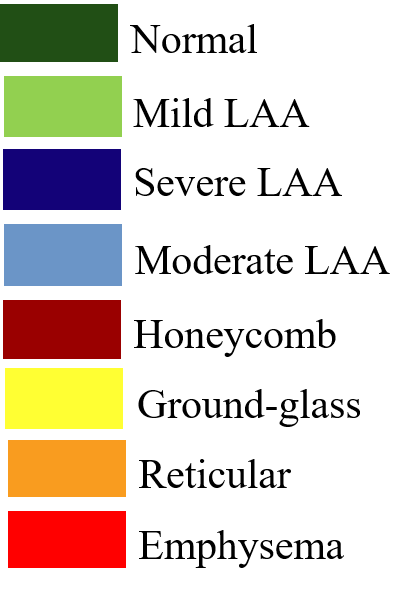
\includegraphics{Appendix/Image_AppexC/ClassifiedColor_new.png}}% get image width, trim={<left> <lower> <right> <upper>}
    \begin{overpic}[height=1.78in,trim={{.0\wd0} {.0\wd0} {.0\wd0} {.0\wd0}},clip]{Appendix/Image_AppexC/ClassifiedColor_new.png}
    \end{overpic}
\end{subfigure}
\caption{Classified data (top row) and mapped data (bottom row) of three time points of case IPF6. (a) The first time point, scan time: 0 month. (b) The second time point, scan time: 15 months. (c) The third time point, scan time: 20 months}
\label{fig:IPF6MappingResult}
\end{figure}
\end{landscape}
\restoregeometry

\newgeometry{bottom=4cm} %set the left margin of page
\begin{landscape}
\begin{figure}[htbp]
\begin{subfigure}{6.5cm}
    \makebox[60pt]{\raisebox{50pt}{\rotatebox[origin=c]{0}{\minibox{IPF9 Classified\\ data}}}}%
    \sbox0{\includegraphics{Appendix/Image_AppexC/IPF9_ClassifiedData_Time1.png}}% get image width, trim={<left> <lower> <right> <upper>}
    \begin{overpic}[height=1.62in,trim={{.0\wd0} {.0\wd0} {.0\wd0} {.0\wd0}},clip]{Appendix/Image_AppexC/IPF9_ClassifiedData_Time1.png}
    \end{overpic}
    \makebox[60pt]{\raisebox{60pt}{\rotatebox[origin=c]{0}{\minibox{IPF9 Mapped\\ data}}}}% \makebox:change left space, \raisebox: change upper space
    \begin{overpic}[height=1.64in,trim={{.0\wd0} {.0\wd0} {.0\wd0} {.0\wd0}},clip]{Appendix/Image_AppexC/IPF9_MappedData_Time1.png}
    \end{overpic}
    \caption{Time point 1}
		\label{fig:IPF9MappingResult-a}
\end{subfigure}\hspace{0.3cm}
\begin{subfigure}{4.8cm}
    \sbox0{\includegraphics{Appendix/Image_AppexC/IPF9_ClassifiedData_Time2.png}}% get image width, trim={<left> <lower> <right> <upper>}
    \begin{overpic}[height=1.59in,trim={{.0\wd0} {.0\wd0} {.0\wd0} {.0\wd0}},clip]{Appendix/Image_AppexC/IPF9_ClassifiedData_Time2.png}
    \end{overpic}
    \begin{overpic}[height=1.67in,trim={{.0\wd0} {.0\wd0} {.0\wd0} {.0\wd0}},clip]{Appendix/Image_AppexC/IPF9_MappedData_Time2.png}
    \end{overpic}
    \caption{Time point 2}
		\label{fig:IPF9MappingResult-b}
\end{subfigure}\hspace{0.3cm}
\begin{subfigure}{4.8cm}
    \sbox0{\includegraphics{Appendix/Image_AppexC/IPF9_ClassifiedData_Time3.png}}% get image width, trim={<left> <lower> <right> <upper>}
    \begin{overpic}[height=1.56in,trim={{.0\wd0} {.0\wd0} {.0\wd0} {.0\wd0}},clip]{Appendix/Image_AppexC/IPF9_ClassifiedData_Time3.png}
    \end{overpic}
    \begin{overpic}[height=1.66in,trim={{.0\wd0} {.0\wd0} {.0\wd0} {.0\wd0}},clip]{Appendix/Image_AppexC/IPF9_MappedData_Time3.png}
    \end{overpic}
    \caption{Time point 3}
		\label{fig:IPF9MappingResult-c}
\end{subfigure}
\begin{subfigure}{2cm}
    \makebox[30pt]{\raisebox{100pt}{\rotatebox[origin=c]{0}{\minibox{\\}}}}
    \sbox0{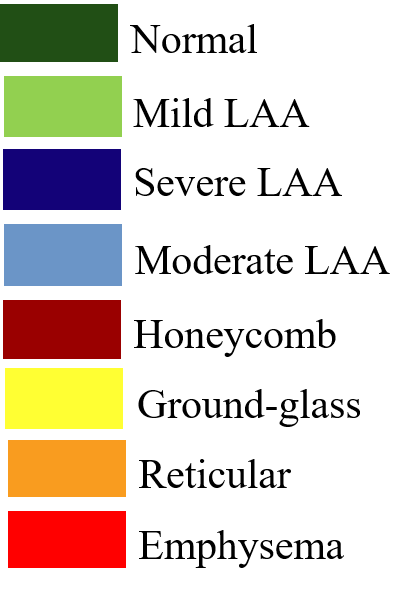
\includegraphics{Appendix/Image_AppexC/ClassifiedColor_new.png}}% get image width, trim={<left> <lower> <right> <upper>}
    \begin{overpic}[height=1.78in,trim={{.0\wd0} {.0\wd0} {.0\wd0} {.0\wd0}},clip]{Appendix/Image_AppexC/ClassifiedColor_new.png}
    \end{overpic}
\end{subfigure}
\caption{Classified data (top row) and mapped data (bottom row) of three time points of case IPF9. (a) The first time point, scan time: 0 month. (b) The second time point, scan time: 6 months. (c) The third time point, scan time: 19 months}
\label{fig:IPF9MappingResult}
\end{figure}
\end{landscape}
\restoregeometry

\newgeometry{bottom=4cm} %set the left margin of page
\begin{landscape}
\begin{figure}[htbp]
\begin{subfigure}{6.5cm}
    \makebox[60pt]{\raisebox{50pt}{\rotatebox[origin=c]{0}{\minibox{IPF15 Classified\\ data}}}}%
    \sbox0{\includegraphics{Appendix/Image_AppexC/IPF15_ClassifiedData_Time1.png}}% get image width, trim={<left> <lower> <right> <upper>}
    \begin{overpic}[height=1.64in,trim={{.0\wd0} {.0\wd0} {.0\wd0} {.0\wd0}},clip]{Appendix/Image_AppexC/IPF15_ClassifiedData_Time1.png}
    \end{overpic}
    \makebox[60pt]{\raisebox{60pt}{\rotatebox[origin=c]{0}{\minibox{IPF15 Mapped\\ data}}}}% \makebox:change left space, \raisebox: change upper space
    \begin{overpic}[height=1.66in,trim={{.0\wd0} {.0\wd0} {.0\wd0} {.0\wd0}},clip]{Appendix/Image_AppexC/IPF15_MappedData_Time1.png}
    \end{overpic}
    \caption{Time point 1}
		\label{fig:IPF15MappingResult-a}
\end{subfigure}\hspace{0.3cm}
\begin{subfigure}{4.8cm}
    \sbox0{\includegraphics{Appendix/Image_AppexC/IPF15_ClassifiedData_Time2.png}}% get image width, trim={<left> <lower> <right> <upper>}
    \begin{overpic}[height=1.57in,trim={{.0\wd0} {.0\wd0} {.0\wd0} {.0\wd0}},clip]{Appendix/Image_AppexC/IPF15_ClassifiedData_Time2.png}
    \end{overpic}
    \begin{overpic}[height=1.67in,trim={{.0\wd0} {.0\wd0} {.0\wd0} {.0\wd0}},clip]{Appendix/Image_AppexC/IPF15_MappedData_Time2.png}
    \end{overpic}
    \caption{Time point 2}
		\label{fig:IPF15MappingResult-b}
\end{subfigure}\hspace{0.3cm}
\begin{subfigure}{4.8cm}
    \sbox0{\includegraphics{Appendix/Image_AppexC/IPF15_ClassifiedData_Time3.png}}% get image width, trim={<left> <lower> <right> <upper>}
    \begin{overpic}[height=1.56in,trim={{.0\wd0} {.0\wd0} {.0\wd0} {.0\wd0}},clip]{Appendix/Image_AppexC/IPF15_ClassifiedData_Time3.png}
    \end{overpic}
    \begin{overpic}[height=1.66in,trim={{.0\wd0} {.0\wd0} {.0\wd0} {.0\wd0}},clip]{Appendix/Image_AppexC/IPF15_MappedData_Time3.png}
    \end{overpic}
    \caption{Time point 3}
		\label{fig:IPF15MappingResult-c}
\end{subfigure}
\begin{subfigure}{2cm}
    \makebox[30pt]{\raisebox{100pt}{\rotatebox[origin=c]{0}{\minibox{\\}}}}
    \sbox0{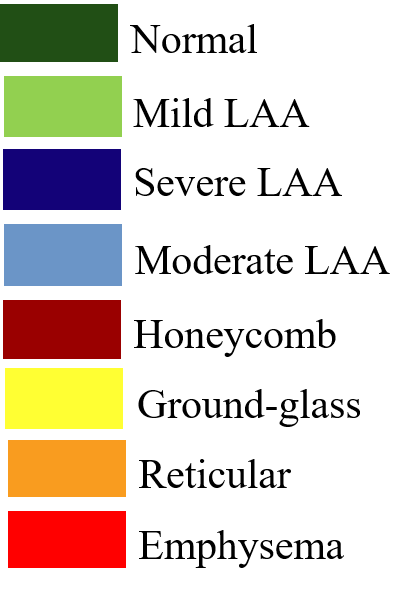
\includegraphics{Appendix/Image_AppexC/ClassifiedColor_new.png}}% get image width, trim={<left> <lower> <right> <upper>}
    \begin{overpic}[height=1.78in,trim={{.0\wd0} {.0\wd0} {.0\wd0} {.0\wd0}},clip]{Appendix/Image_AppexC/ClassifiedColor_new.png}
    \end{overpic}
\end{subfigure}
\caption{Classified data (top row) and mapped data (bottom row) of three time points of case IPF15. (a) The first time point, scan time: 0 month. (b) The second time point, scan time: 13 months. (c) The third time point, scan time: 76 months}
\label{fig:IPF15MappingResult}
\end{figure}
\end{landscape}
\restoregeometry

\newgeometry{bottom=4cm} %set the left margin of page
\begin{landscape}
\begin{figure}[htbp]
\begin{subfigure}{6.5cm}
    \makebox[60pt]{\raisebox{50pt}{\rotatebox[origin=c]{0}{\minibox{IPF21 Classified\\ data}}}}%
    \sbox0{\includegraphics{Appendix/Image_AppexC/IPF21_ClassifiedData_Time1.png}}% get image width, trim={<left> <lower> <right> <upper>}
    \begin{overpic}[height=1.66in,trim={{.0\wd0} {.0\wd0} {.0\wd0} {.0\wd0}},clip]{Appendix/Image_AppexC/IPF21_ClassifiedData_Time1.png}
    \end{overpic}
    \makebox[60pt]{\raisebox{60pt}{\rotatebox[origin=c]{0}{\minibox{IPF21 Mapped\\ data}}}}% \makebox:change left space, \raisebox: change upper space
    \begin{overpic}[height=1.66in,trim={{.0\wd0} {.0\wd0} {.0\wd0} {.0\wd0}},clip]{Appendix/Image_AppexC/IPF21_MappedData_Time1.png}
    \end{overpic}
    \caption{Time point 1}
		\label{fig:IPF21MappingResult-a}
\end{subfigure}\hspace{0.3cm}
\begin{subfigure}{4.8cm}
    \sbox0{\includegraphics{Appendix/Image_AppexC/IPF21_ClassifiedData_Time2.png}}% get image width, trim={<left> <lower> <right> <upper>}
    \begin{overpic}[height=1.62in,trim={{.0\wd0} {.0\wd0} {.0\wd0} {.0\wd0}},clip]{Appendix/Image_AppexC/IPF21_ClassifiedData_Time2.png}
    \end{overpic}
    \begin{overpic}[height=1.67in,trim={{.0\wd0} {.0\wd0} {.0\wd0} {.0\wd0}},clip]{Appendix/Image_AppexC/IPF21_MappedData_Time2.png}
    \end{overpic}
    \caption{Time point 2}
		\label{fig:IPF21MappingResult-b}
\end{subfigure}\hspace{0.3cm}
\begin{subfigure}{4.8cm}
    \sbox0{\includegraphics{Appendix/Image_AppexC/IPF21_ClassifiedData_Time3.png}}% get image width, trim={<left> <lower> <right> <upper>}
    \begin{overpic}[height=1.61in,trim={{.0\wd0} {.0\wd0} {.0\wd0} {.0\wd0}},clip]{Appendix/Image_AppexC/IPF21_ClassifiedData_Time3.png}
    \end{overpic}
    \begin{overpic}[height=1.66in,trim={{.0\wd0} {.0\wd0} {.0\wd0} {.0\wd0}},clip]{Appendix/Image_AppexC/IPF21_MappedData_Time3.png}
    \end{overpic}
    \caption{Time point 3}
		\label{fig:IPF21MappingResult-c}
\end{subfigure}
\begin{subfigure}{2cm}
    \makebox[30pt]{\raisebox{100pt}{\rotatebox[origin=c]{0}{\minibox{\\}}}}
    \sbox0{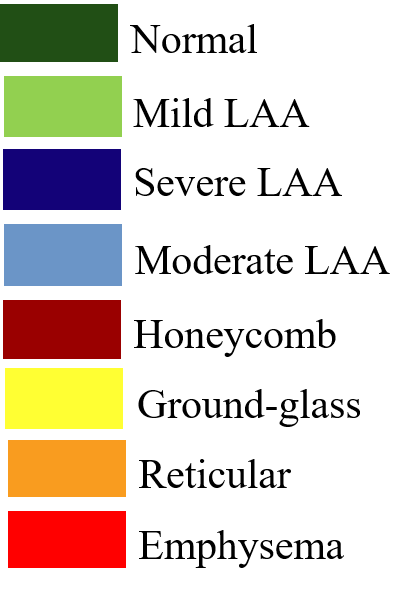
\includegraphics{Appendix/Image_AppexC/ClassifiedColor_new.png}}% get image width, trim={<left> <lower> <right> <upper>}
    \begin{overpic}[height=1.78in,trim={{.0\wd0} {.0\wd0} {.0\wd0} {.0\wd0}},clip]{Appendix/Image_AppexC/ClassifiedColor_new.png}
    \end{overpic}
\end{subfigure}
\caption{Classified data (top row) and mapped data (bottom row) of three time points of case IPF21. (a) The first time point, scan time: 0 month. (b) The second time point, scan time: 63 months. (c) The third time point, scan time: 79 months}
\label{fig:IPF21MappingResult}
\end{figure}
\end{landscape}
\restoregeometry

\chapter{Spatial distribution of abnormalities for each patient} \label{AppendixSpatialDistribution}

\section{Basal-to-apical distribution over time for each patient}
\newpage
\begin{figure}[H] 
\centering
\begin{subfigure}{.42\linewidth}% set image scale
  \sbox0{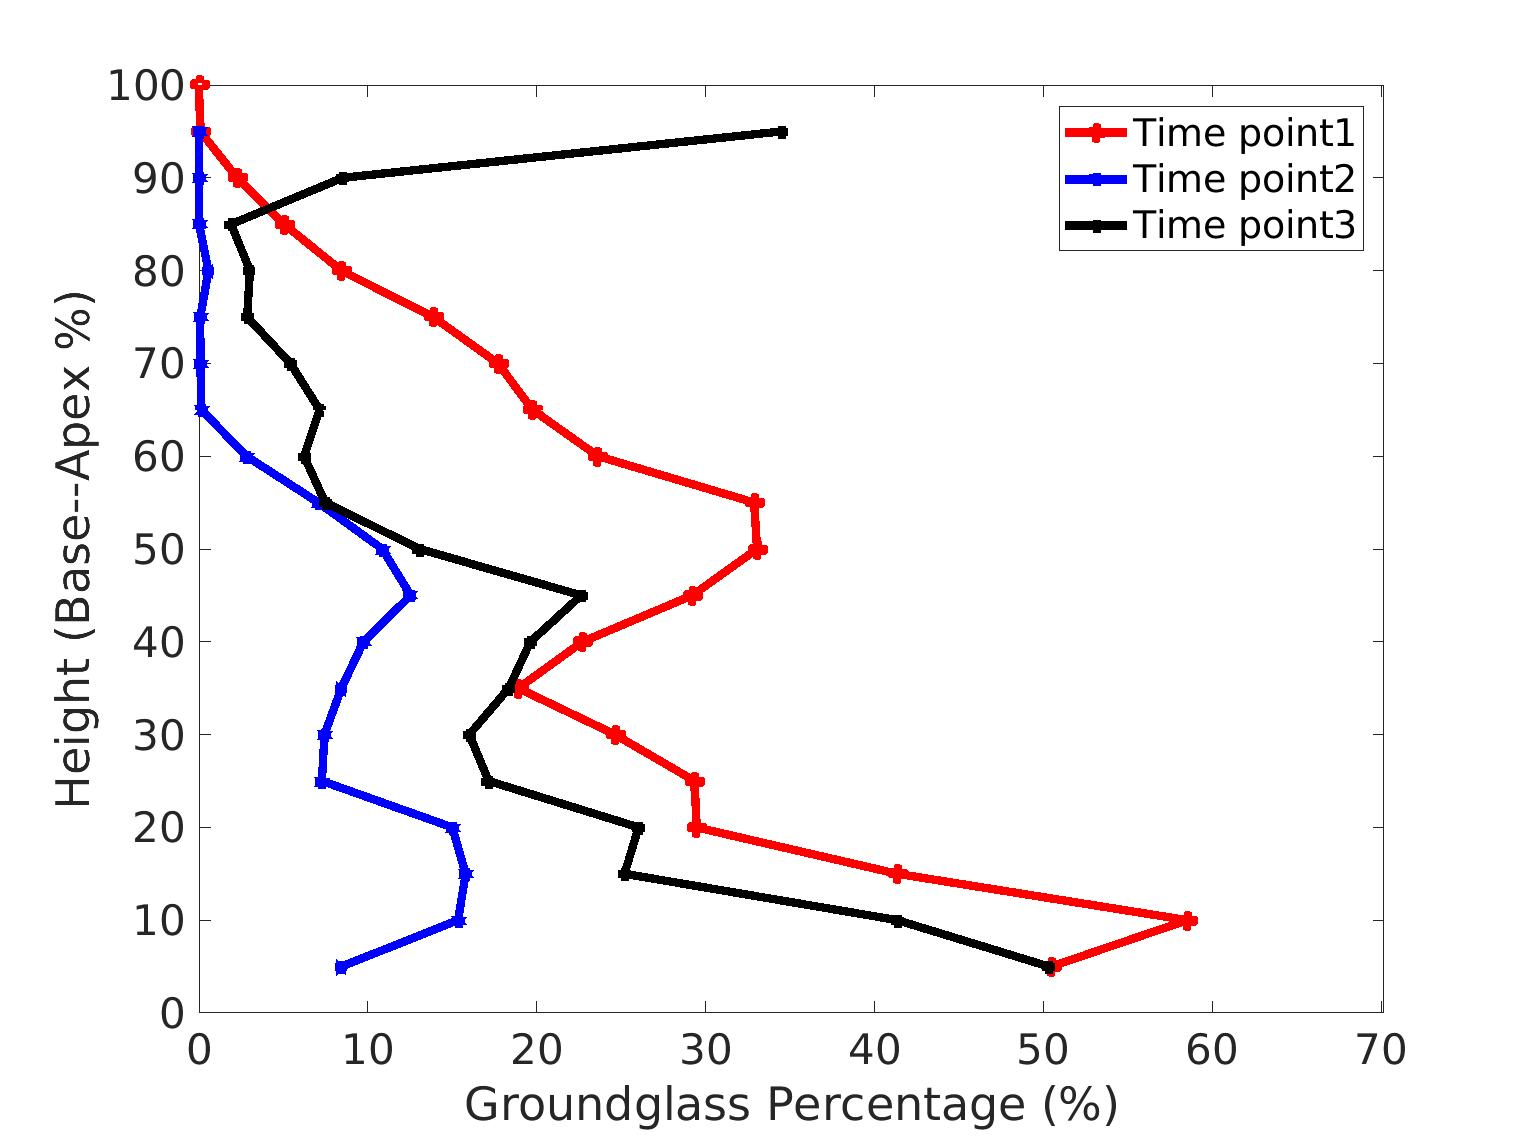
\includegraphics{Appendix/Image_AppexA/BaseToApex/IPF2LeftLungGroundglassDiseaseAgainstHeight.jpg}} 
  %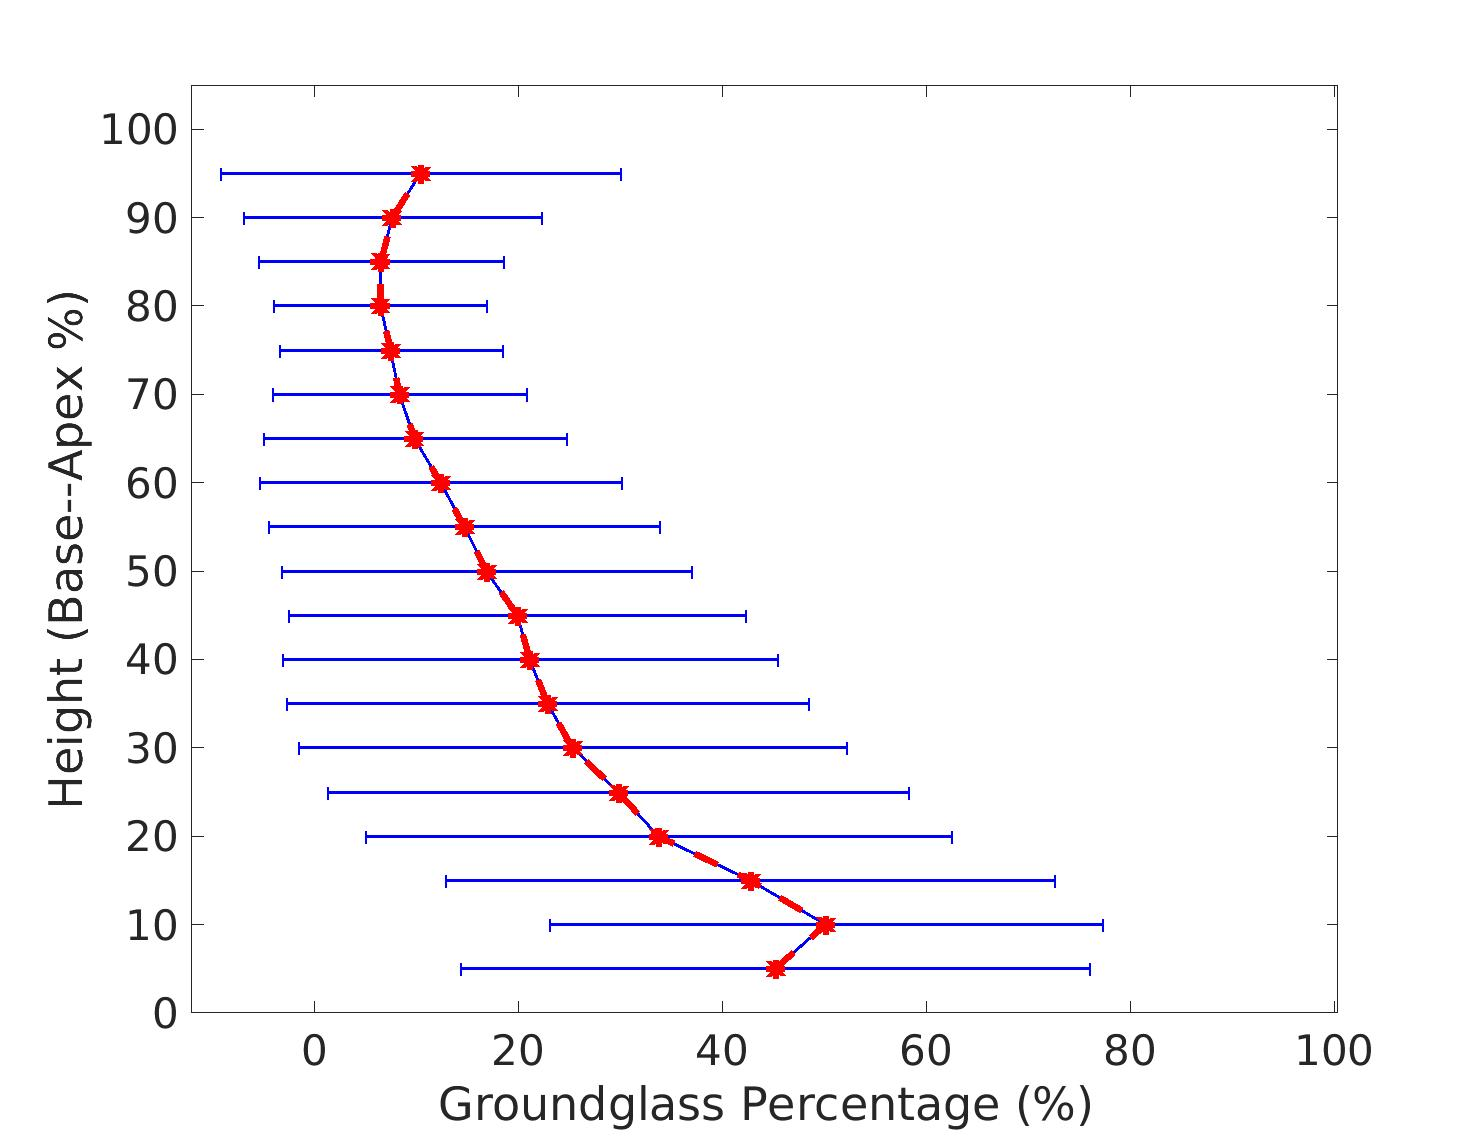
\includegraphics[width=\linewidth,trim={{.0\wd0} {.0\wd0} {.0\wd0} {.0\wd0}},clip]{QuantitativeAnalysis/Image/LeftLungGroundglassDiseaseAgainstHeight.jpg} %trim={<left> <lower> <right> <upper>}, set the cut scale
	\begin{overpic}[width=\linewidth,trim={{.0\wd0} {.0\wd0} {.0\wd0} {.0\wd0}},clip]{Appendix/Image_AppexA/BaseToApex/IPF2LeftLungGroundglassDiseaseAgainstHeight.jpg}
      \put(33,75){\bf{IPF2 left lung}}
  \end{overpic}
  \caption{Left ground-glass}
  \label{fig:IPF2DiseaseAgainstHeight-a} 
\end{subfigure} 
\begin{subfigure}{.42\linewidth}% set image scale
  \sbox0{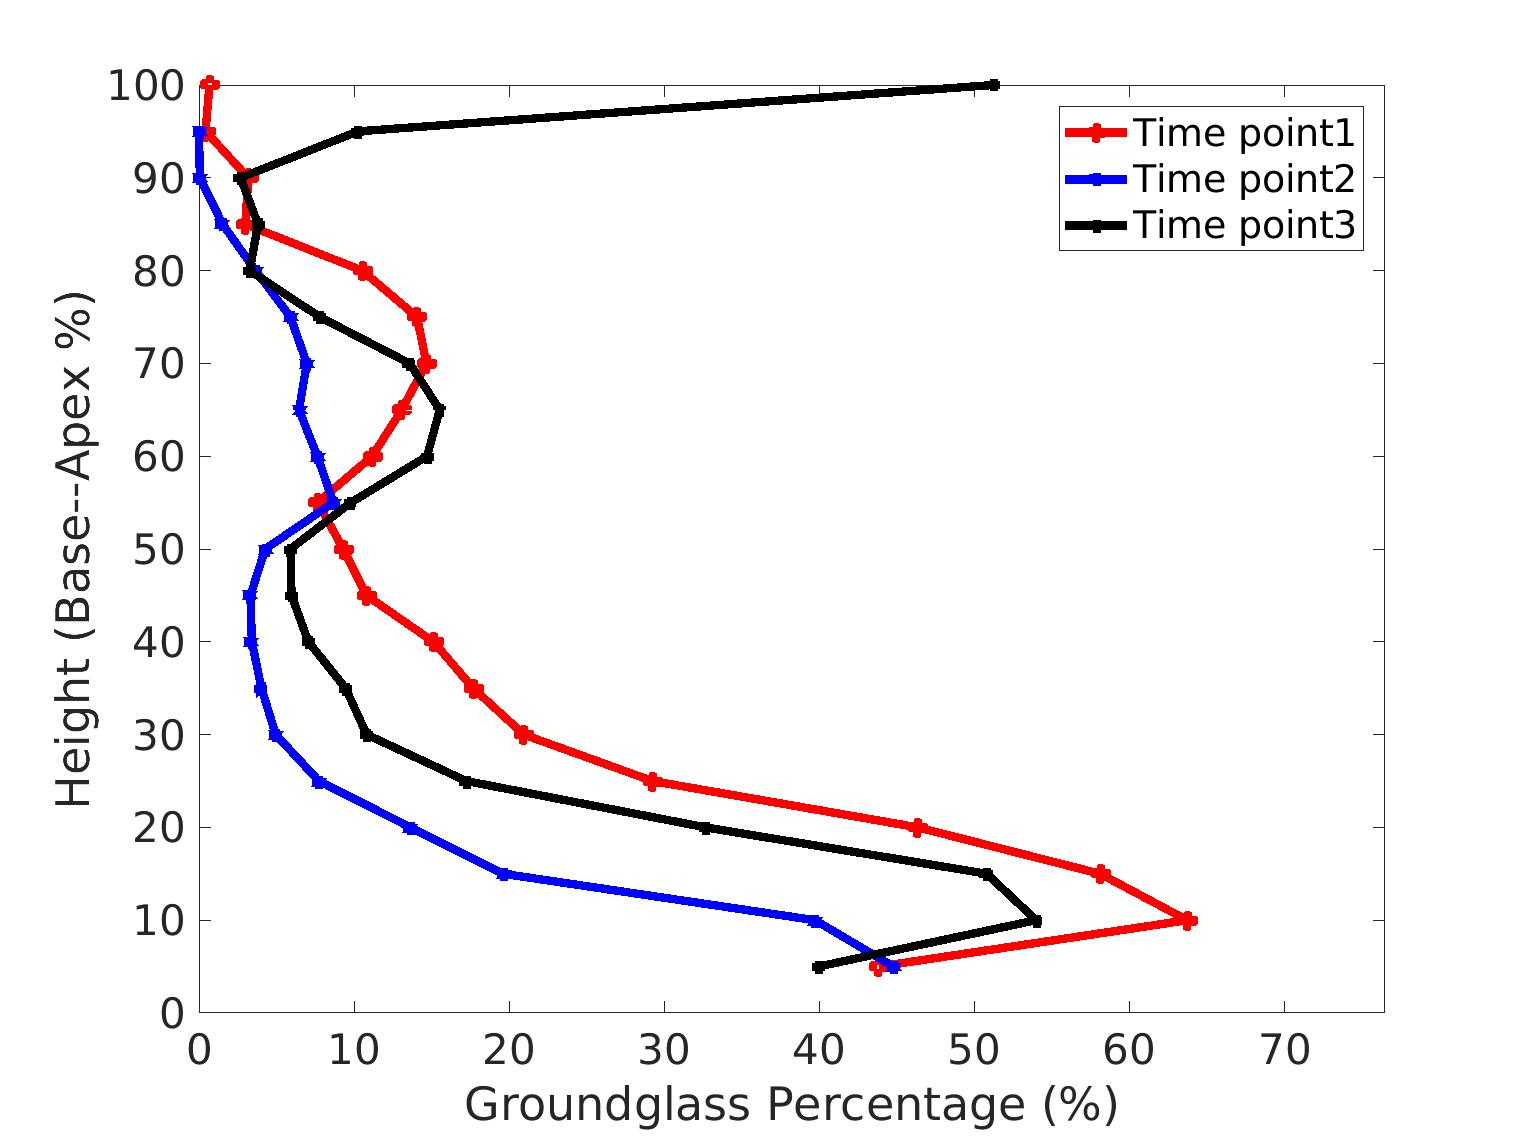
\includegraphics{Appendix/Image_AppexA/BaseToApex/IPF2RightLungGroundglassDiseaseAgainstHeight.jpg}}
  \begin{overpic}[width=\linewidth,trim={{.0\wd0} {.0\wd0} {.0\wd0} {.0\wd0}},clip]{Appendix/Image_AppexA/BaseToApex/IPF2RightLungGroundglassDiseaseAgainstHeight.jpg}
	\put(41,75){\bf{IPF2 right lung}}
  \end{overpic}
  \caption{Right ground-glass}
  \label{fig:IPF2DiseaseAgainstHeight-b}
\end{subfigure}
\begin{subfigure}{.42\linewidth}% set image scale
  \sbox0{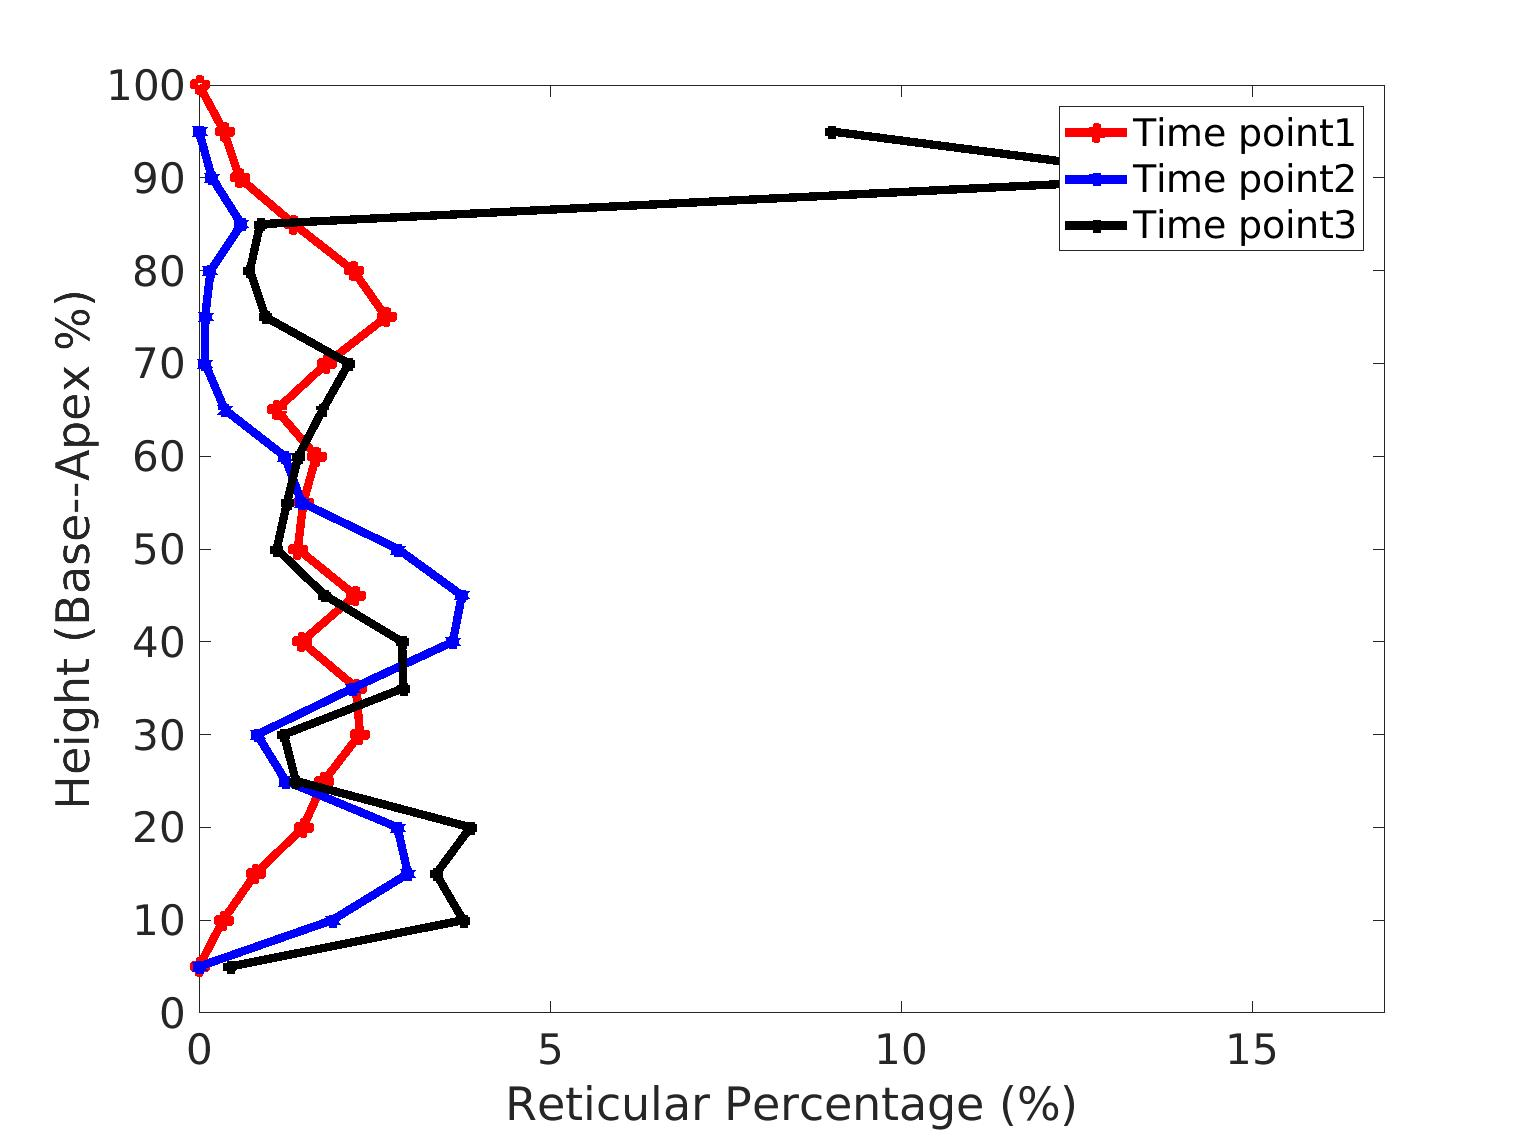
\includegraphics{Appendix/Image_AppexA/BaseToApex/IPF2LeftLungReticularDiseaseAgainstHeight.jpg}} 
  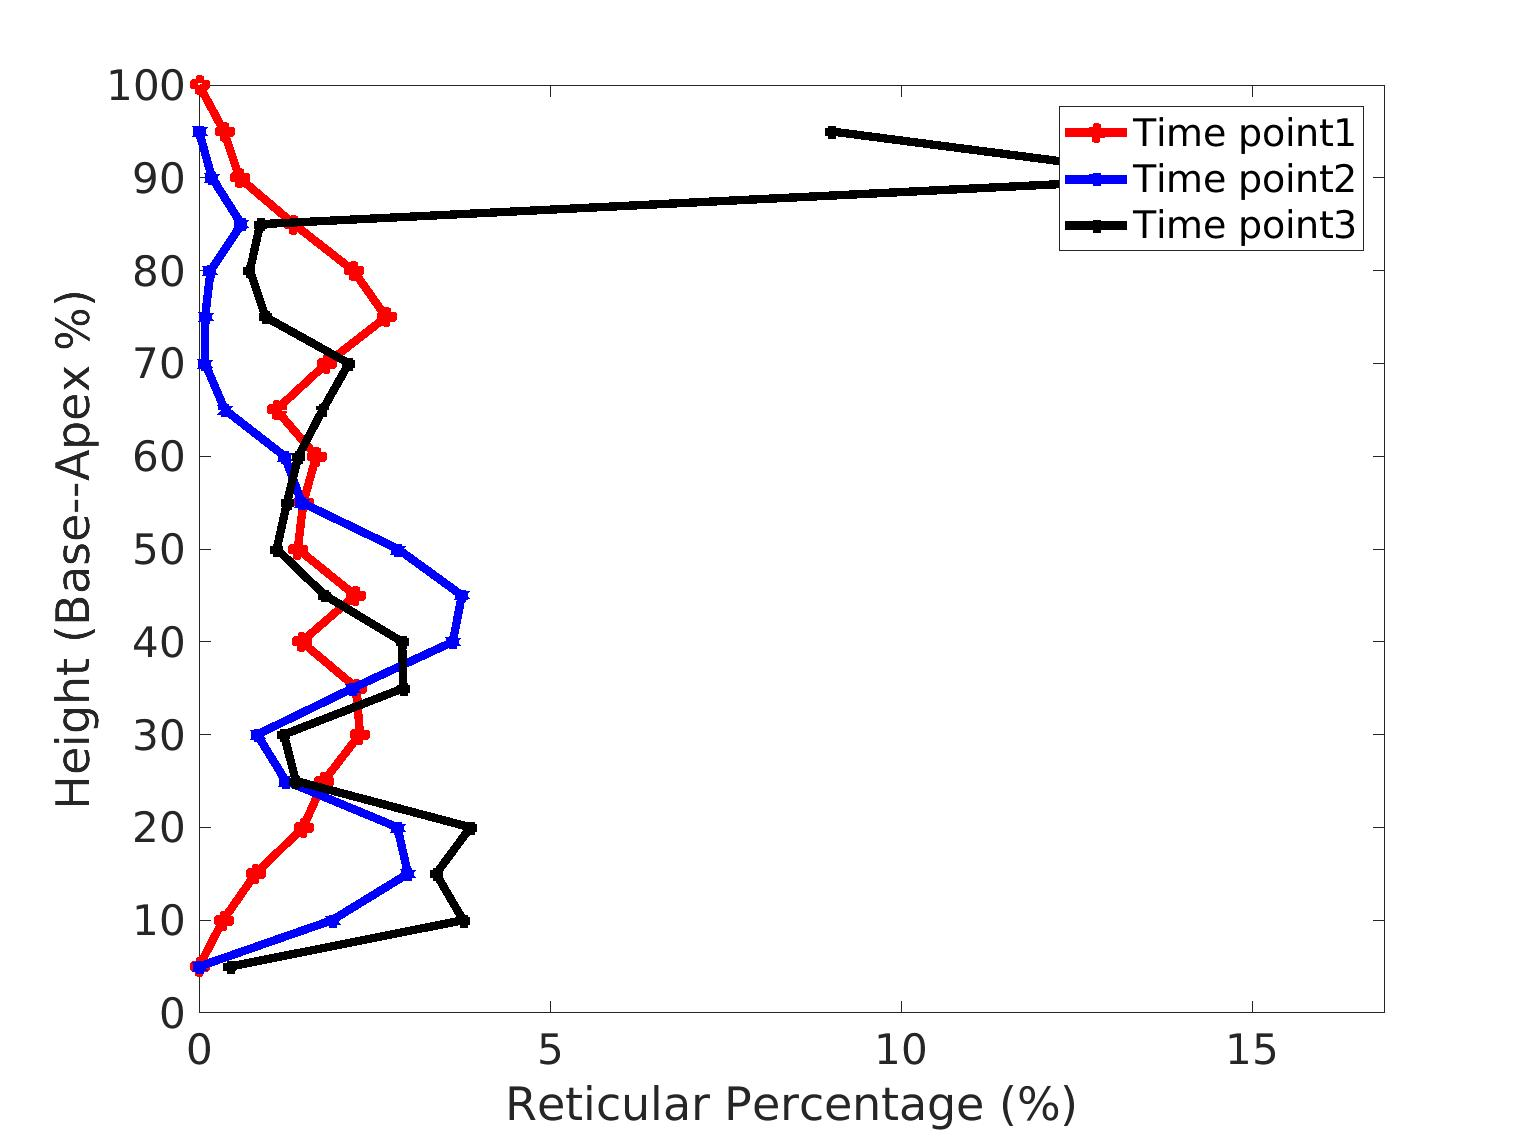
\includegraphics[width=\linewidth,trim={{.0\wd0} {.0\wd0} {.0\wd0} {.0\wd0}},clip]{Appendix/Image_AppexA/BaseToApex/IPF2LeftLungReticularDiseaseAgainstHeight.jpg} %trim={<left> <lower> <right> <upper>}, set the cut scale
  \caption{Left reticular}
  \label{fig:IPF2DiseaseAgainstHeight-c} 
\end{subfigure} 
\begin{subfigure}{.42\linewidth}% set image scale
  \sbox0{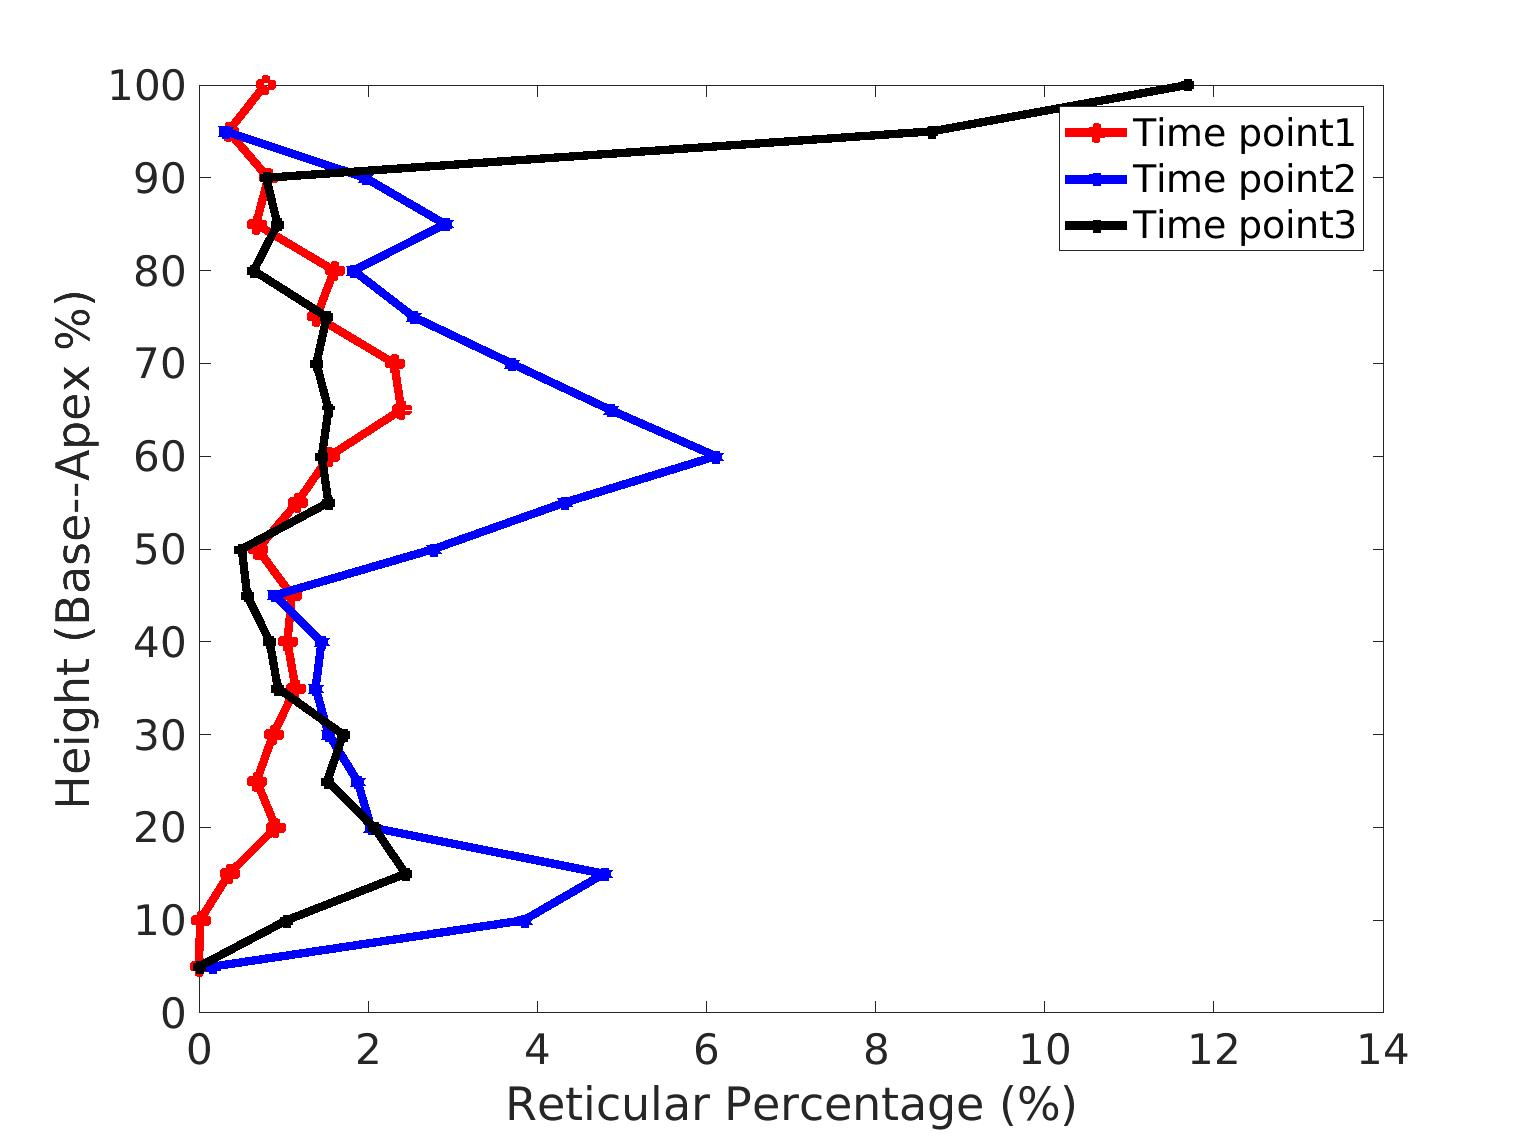
\includegraphics{Appendix/Image_AppexA/BaseToApex/IPF2RightLungReticularDiseaseAgainstHeight.jpg}}
  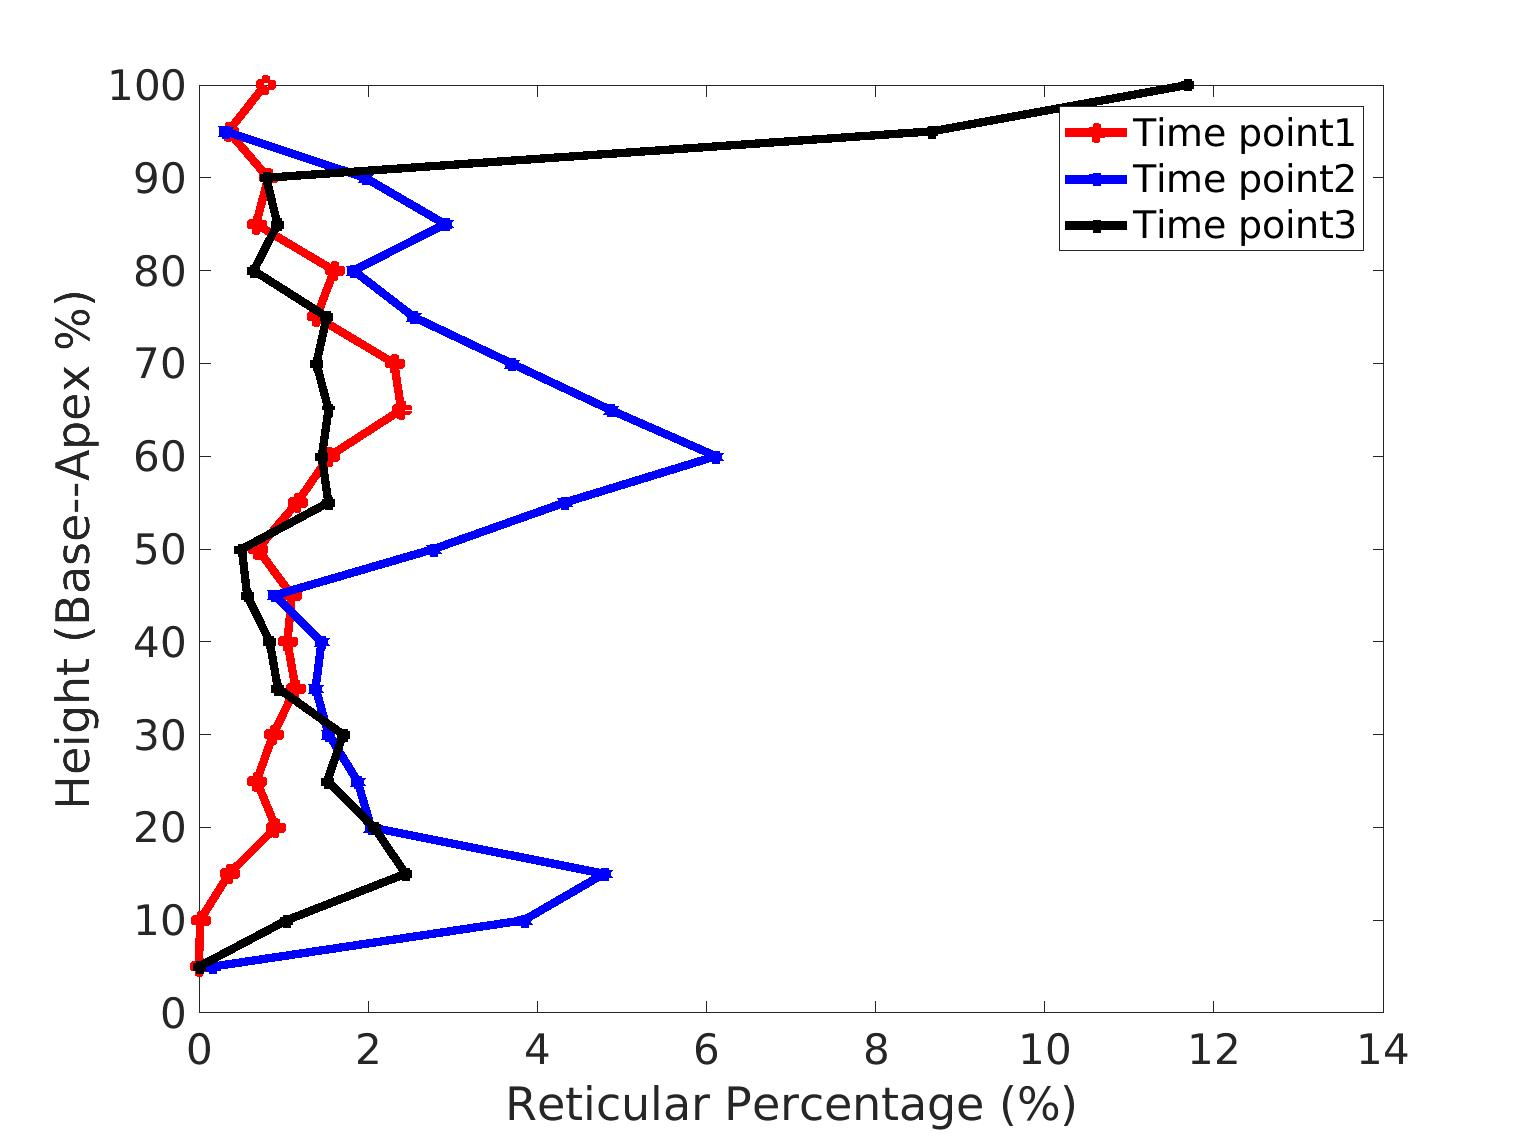
\includegraphics[width=\linewidth,trim={{.0\wd0} {.0\wd0} {.0\wd0} {.0\wd0}},clip]{Appendix/Image_AppexA/BaseToApex/IPF2RightLungReticularDiseaseAgainstHeight.jpg}
  \caption{Right reticular}
  \label{fig:IPF2DiseaseAgainstHeight-d}
\end{subfigure}
\begin{subfigure}{.42\linewidth}% set image scale
  \sbox0{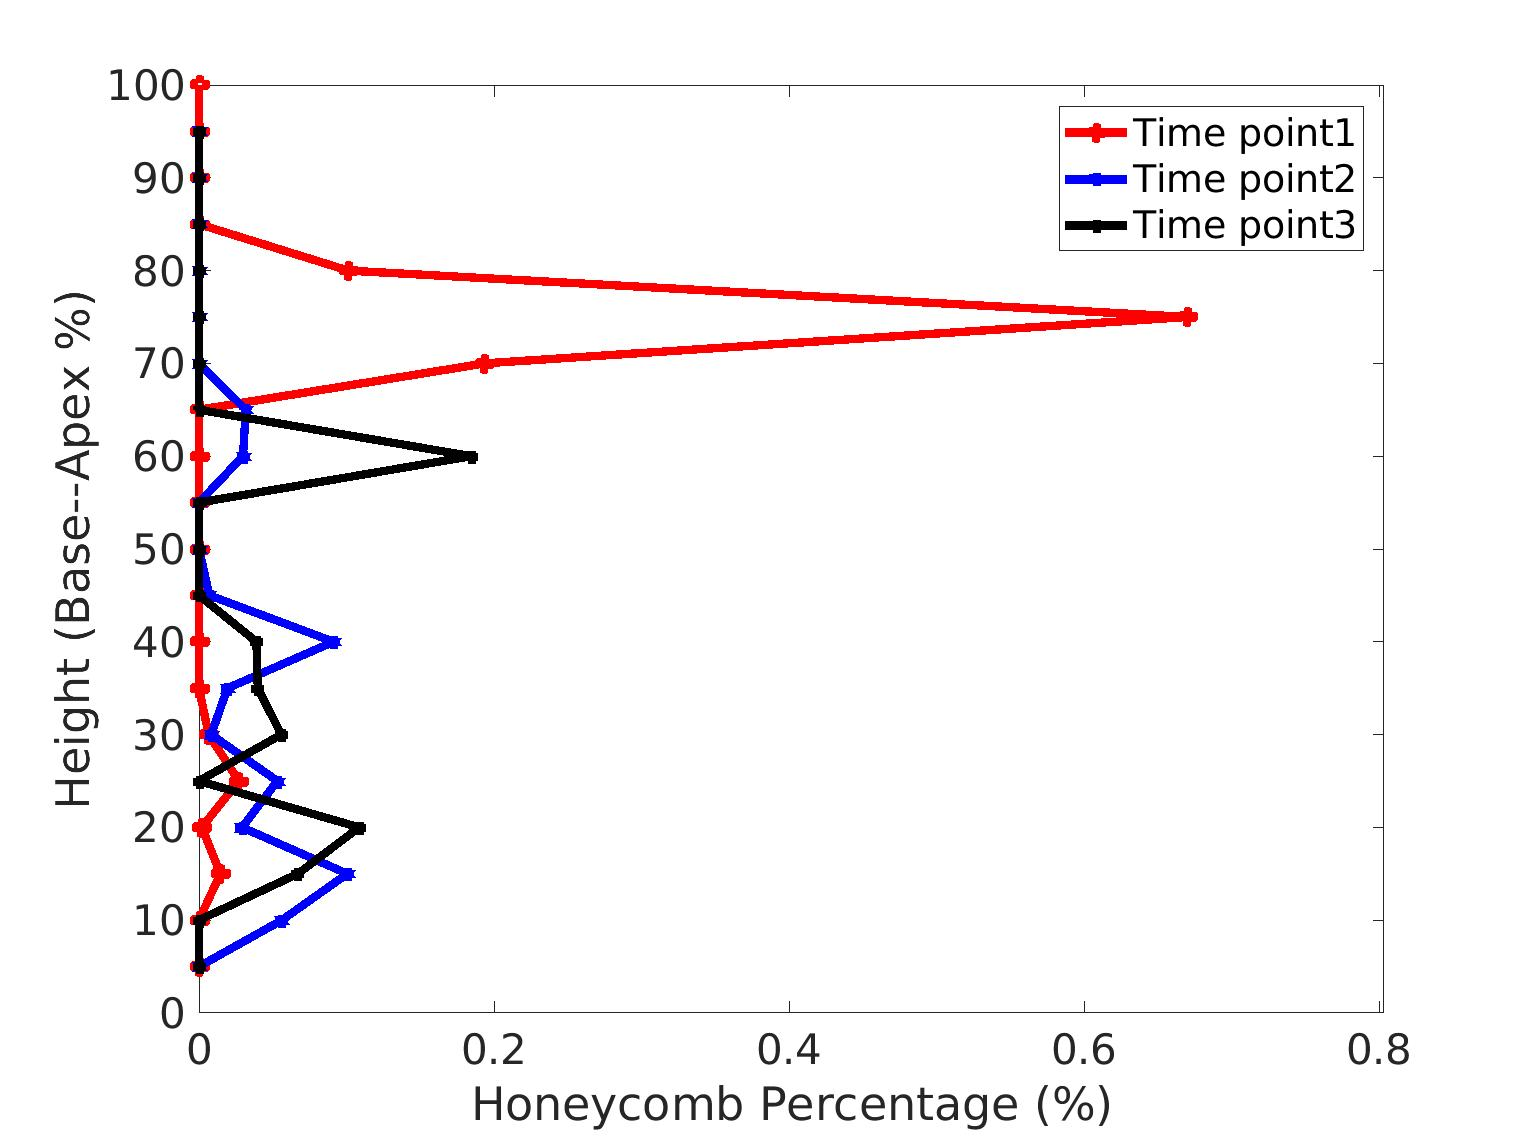
\includegraphics{Appendix/Image_AppexA/BaseToApex/IPF2LeftLungHoneycombDiseaseAgainstHeight.jpg}} 
  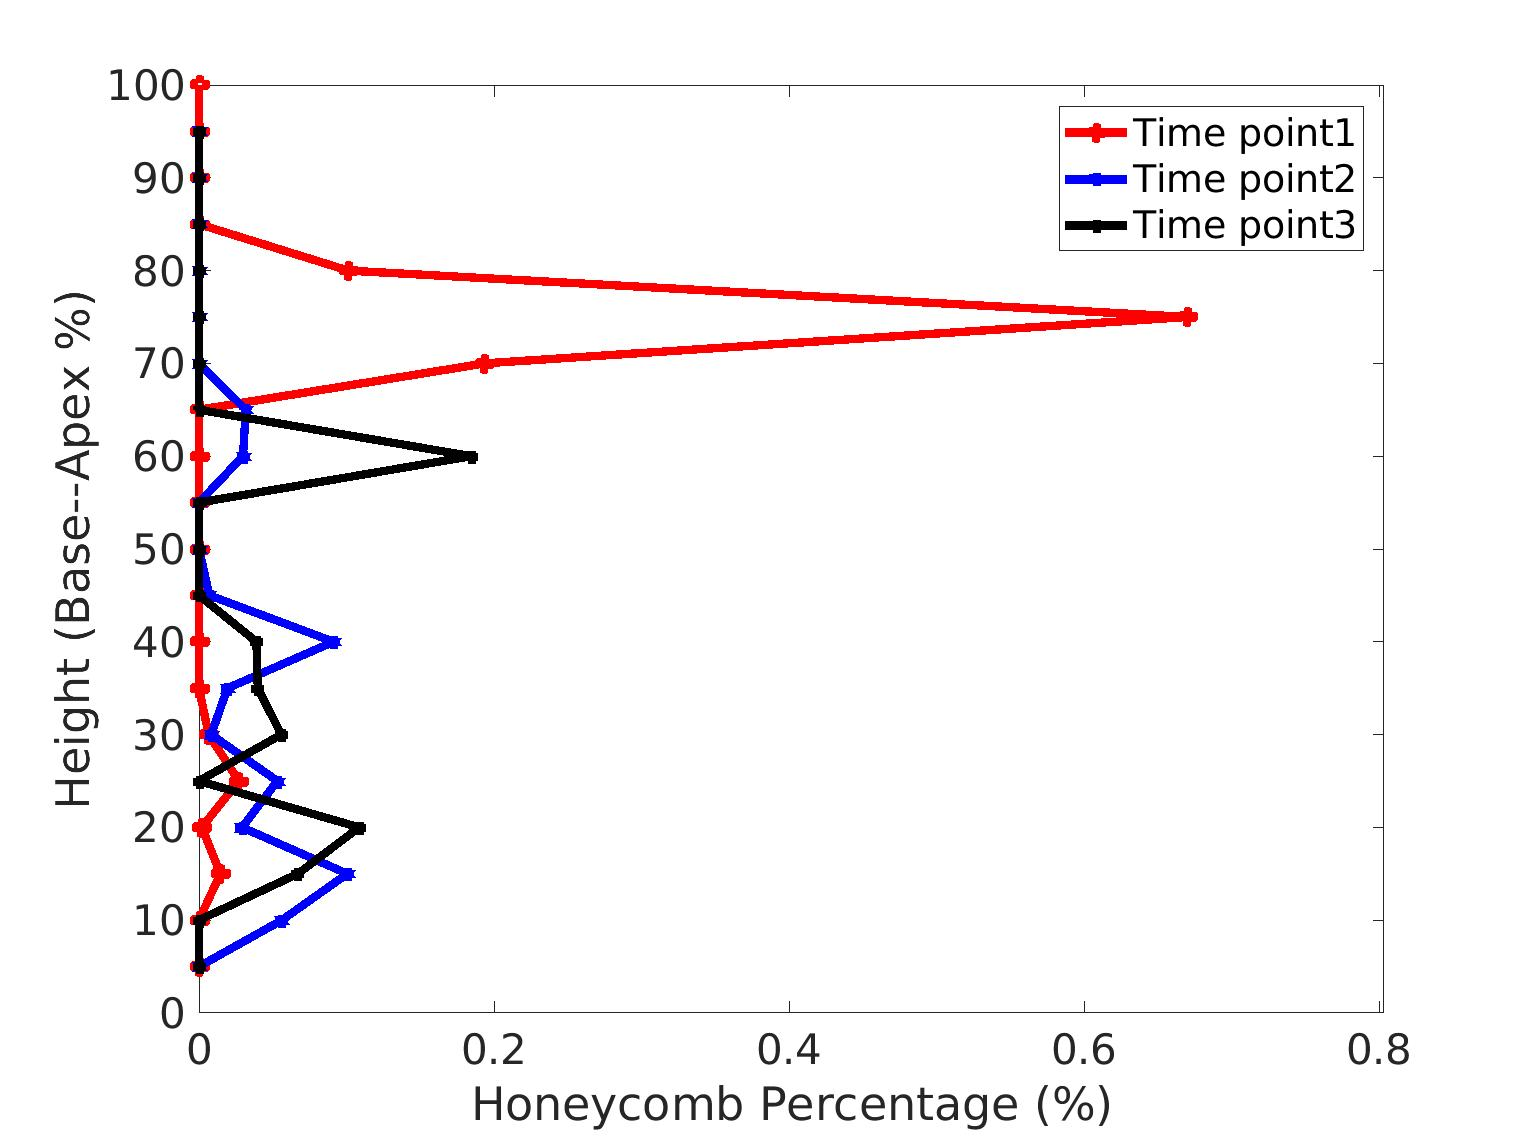
\includegraphics[width=\linewidth,trim={{.0\wd0} {.0\wd0} {.0\wd0} {.0\wd0}},clip]{Appendix/Image_AppexA/BaseToApex/IPF2LeftLungHoneycombDiseaseAgainstHeight.jpg} %trim={<left> <lower> <right> <upper>}, set the cut scale
  \caption{Left honeycomb}
  \label{fig:IPF2DiseaseAgainstHeight-e} 
\end{subfigure} 
\begin{subfigure}{.42\linewidth}% set image scale
  \sbox0{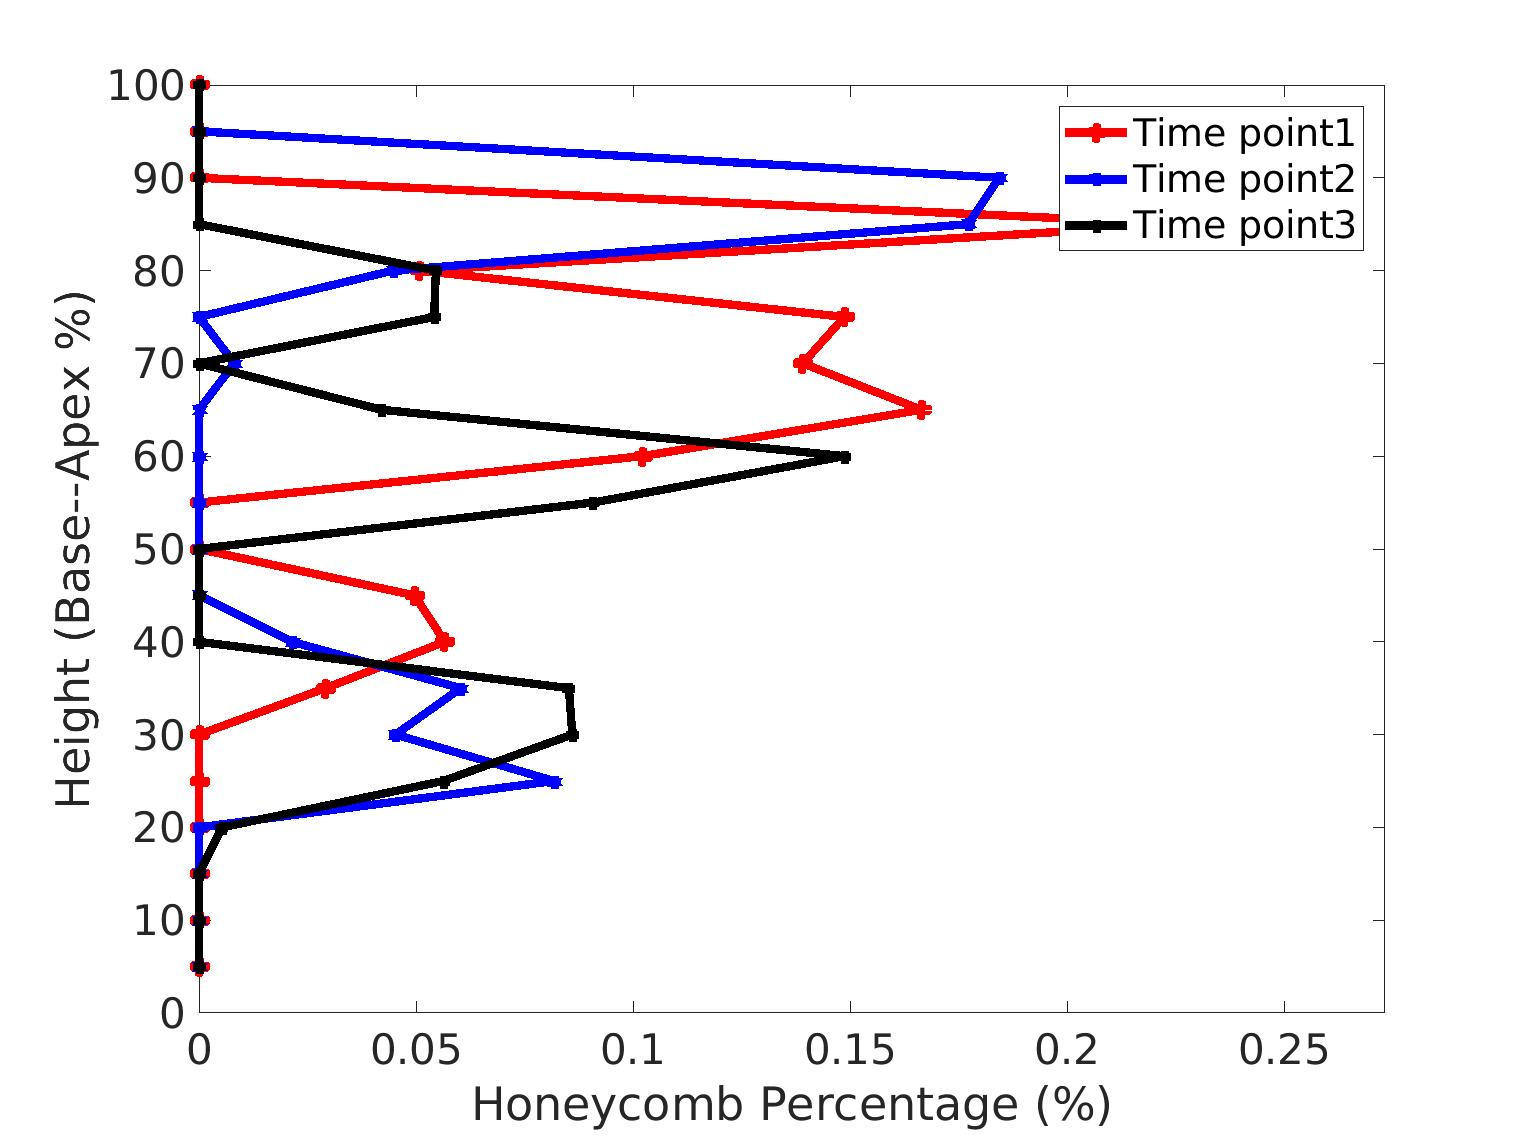
\includegraphics{Appendix/Image_AppexA/BaseToApex/IPF2RightLungHoneycombDiseaseAgainstHeight.jpg}}
  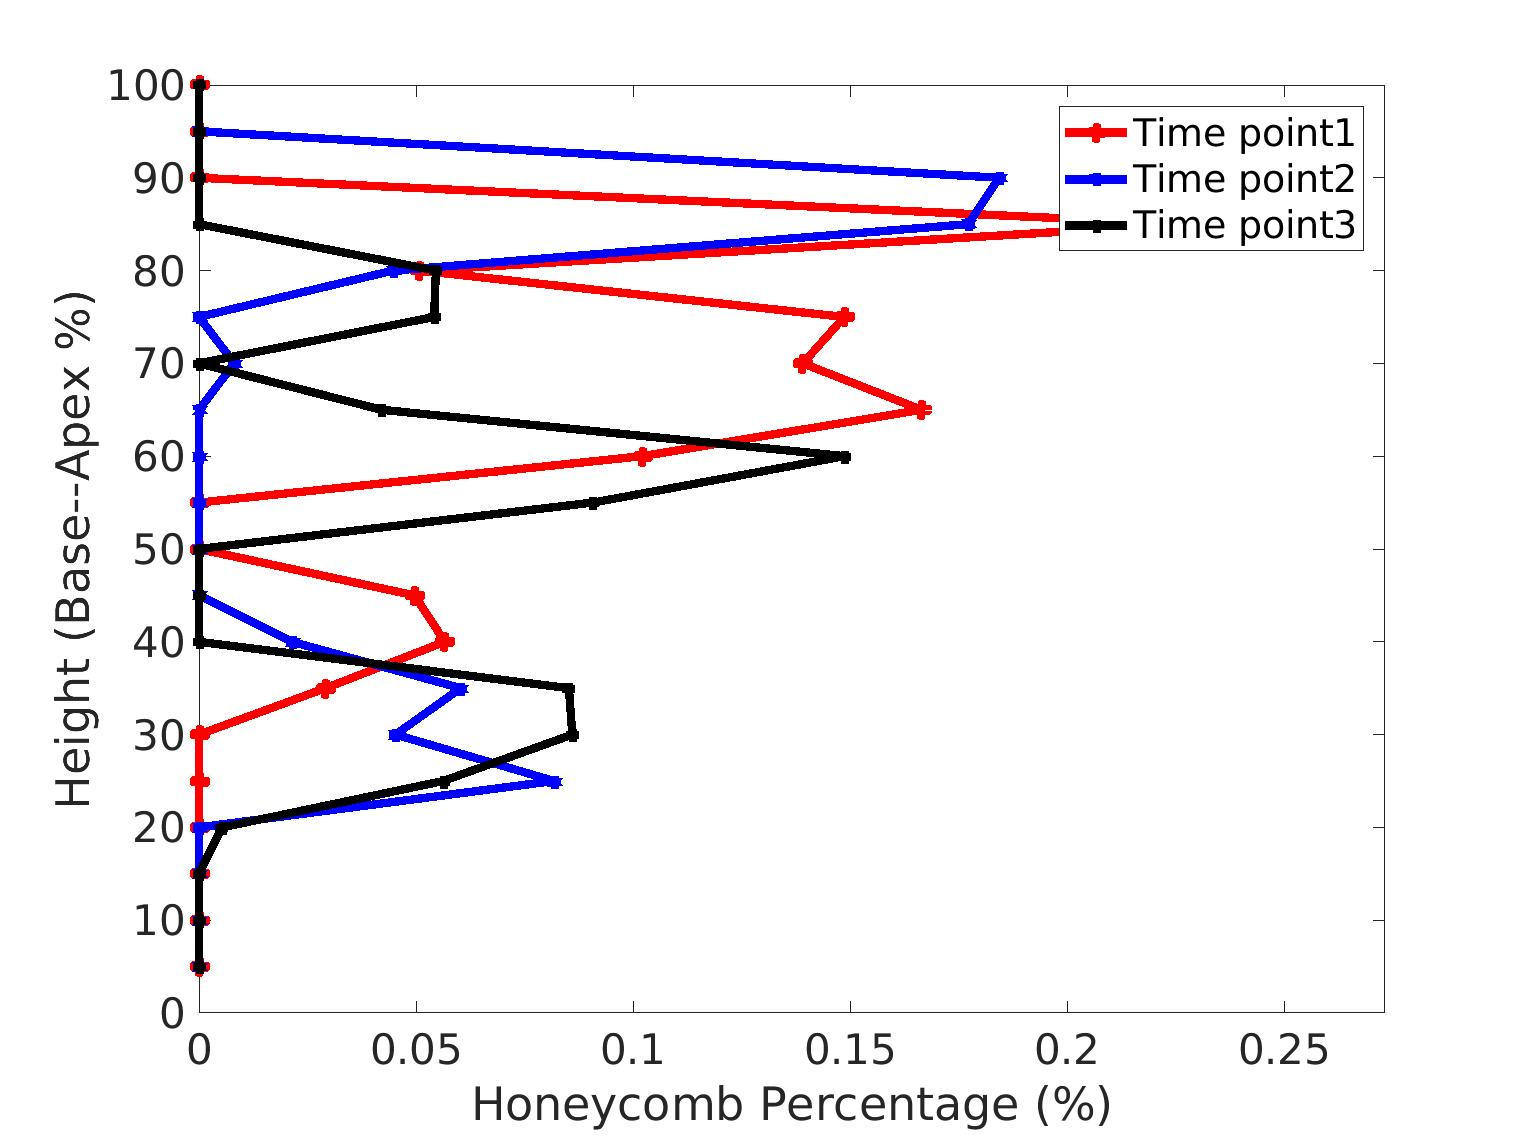
\includegraphics[width=\linewidth,trim={{.0\wd0} {.0\wd0} {.0\wd0} {.0\wd0}},clip]{Appendix/Image_AppexA/BaseToApex/IPF2RightLungHoneycombDiseaseAgainstHeight.jpg}
  \caption{Right honeycomb}
  \label{fig:IPF2DiseaseAgainstHeight-f}
\end{subfigure}
\begin{subfigure}{.42\linewidth}% set image scale
  \sbox0{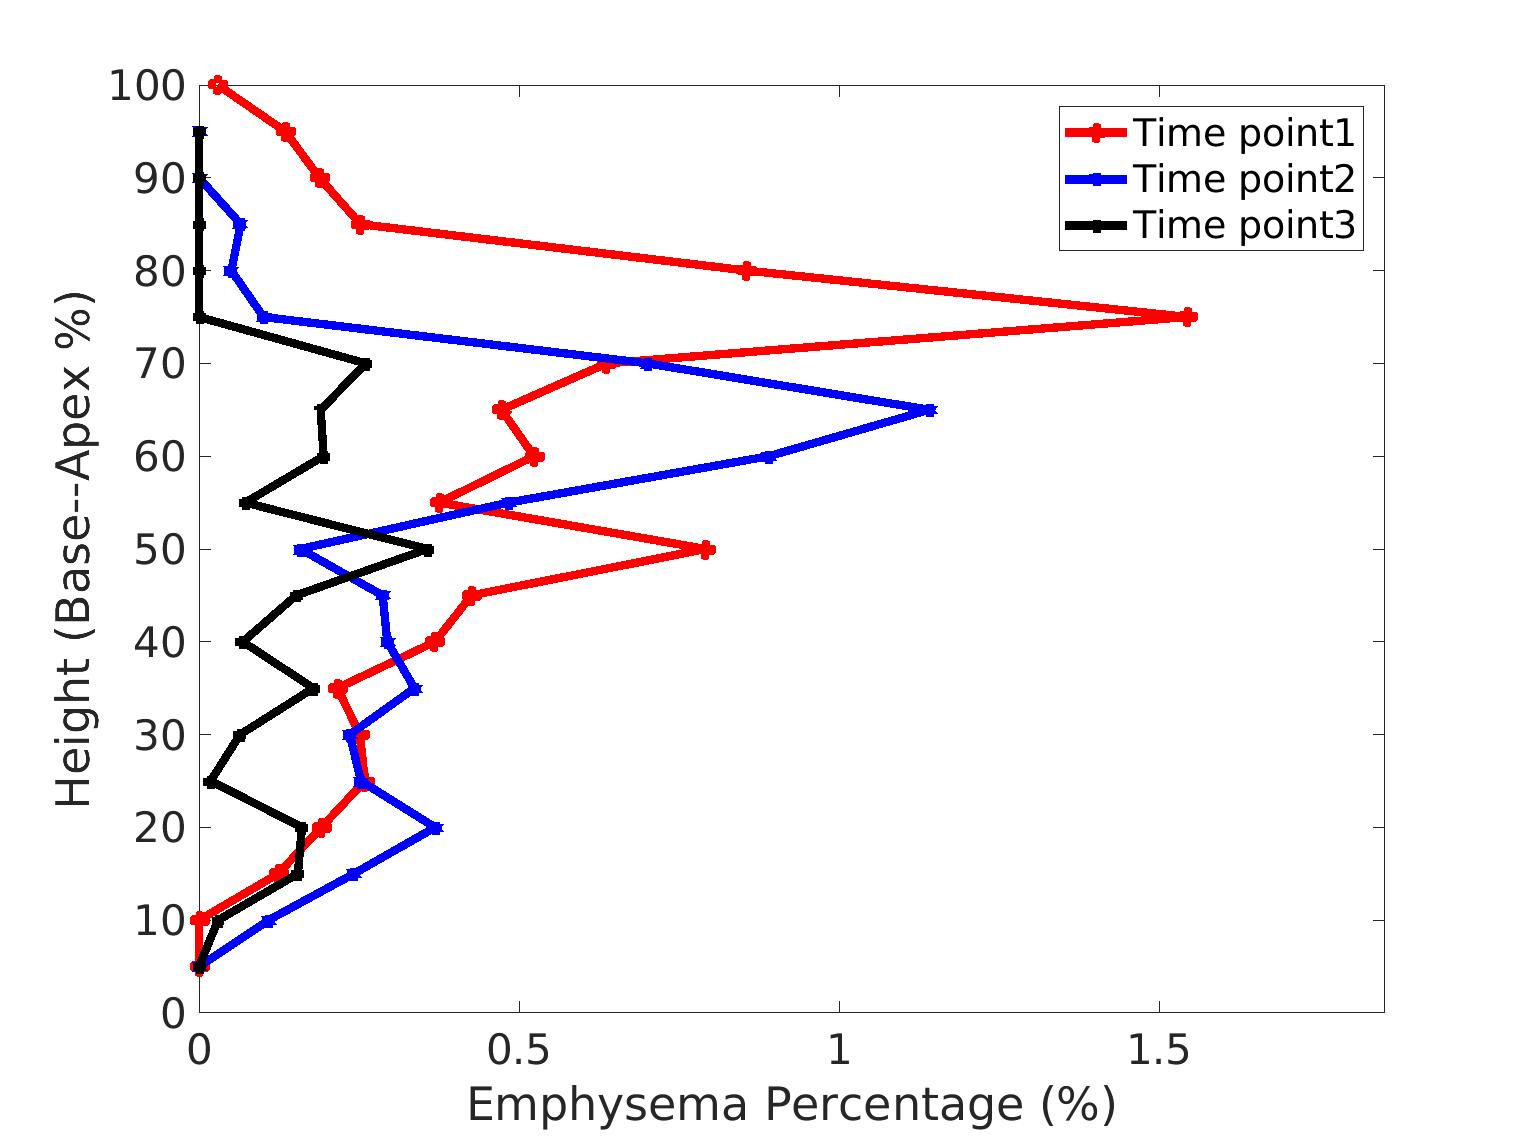
\includegraphics{Appendix/Image_AppexA/BaseToApex/IPF2LeftLungEmphysemaDiseaseAgainstHeight.jpg}} 
  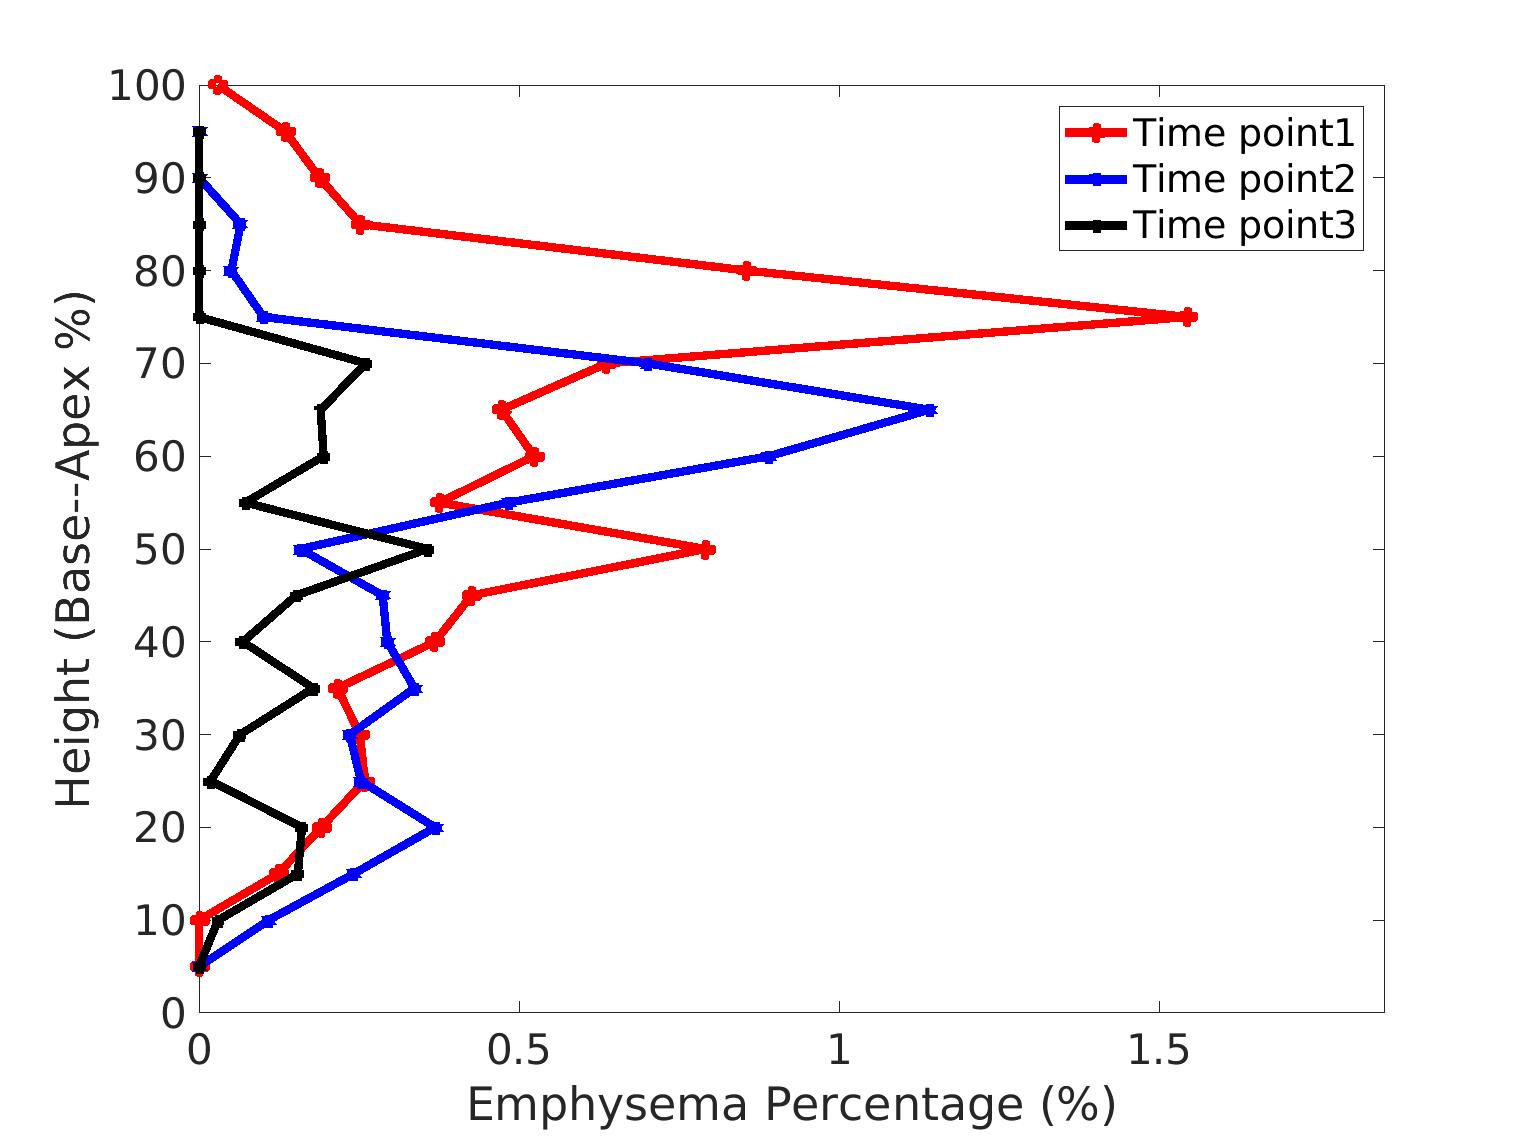
\includegraphics[width=\linewidth,trim={{.0\wd0} {.0\wd0} {.0\wd0} {.0\wd0}},clip]{Appendix/Image_AppexA/BaseToApex/IPF2LeftLungEmphysemaDiseaseAgainstHeight.jpg} %trim={<left> <lower> <right> <upper>}, set the cut scale
  \caption{Left Emphysema}
  \label{fig:IPF2DiseaseAgainstHeight-g} 
\end{subfigure} 
\begin{subfigure}{.42\linewidth}% set image scale
  \sbox0{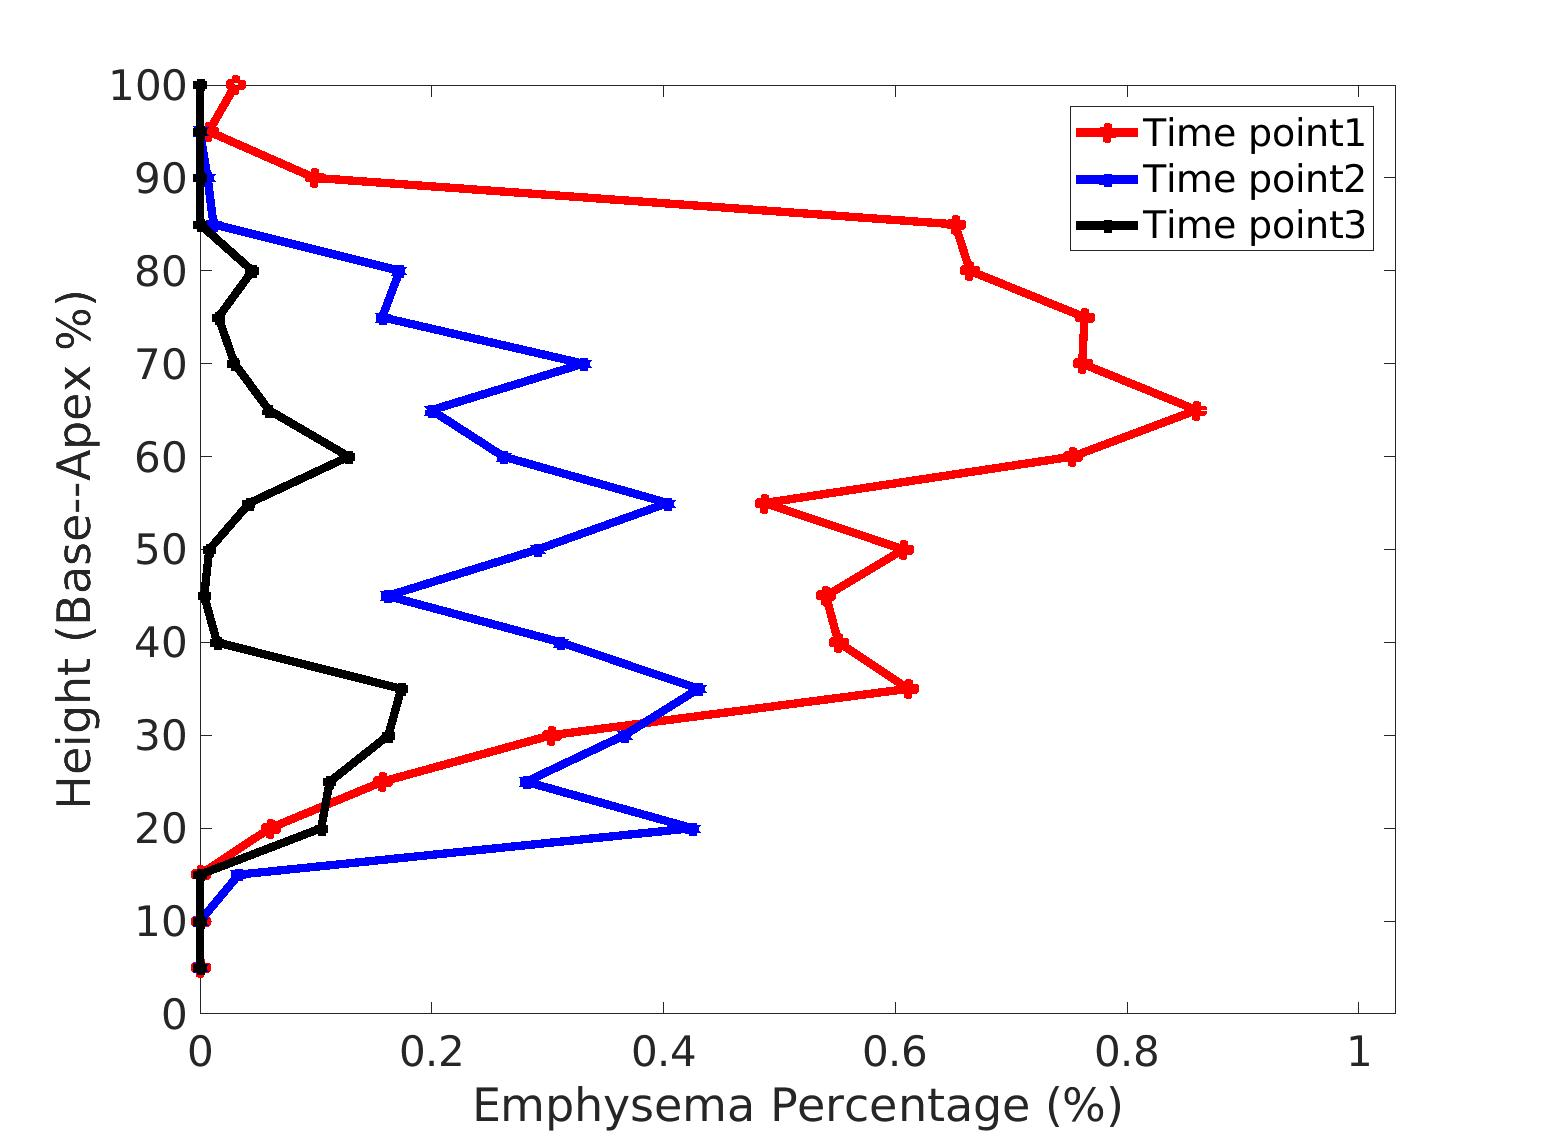
\includegraphics{Appendix/Image_AppexA/BaseToApex/IPF2RightLungEmphysemaDiseaseAgainstHeight.jpg}}
  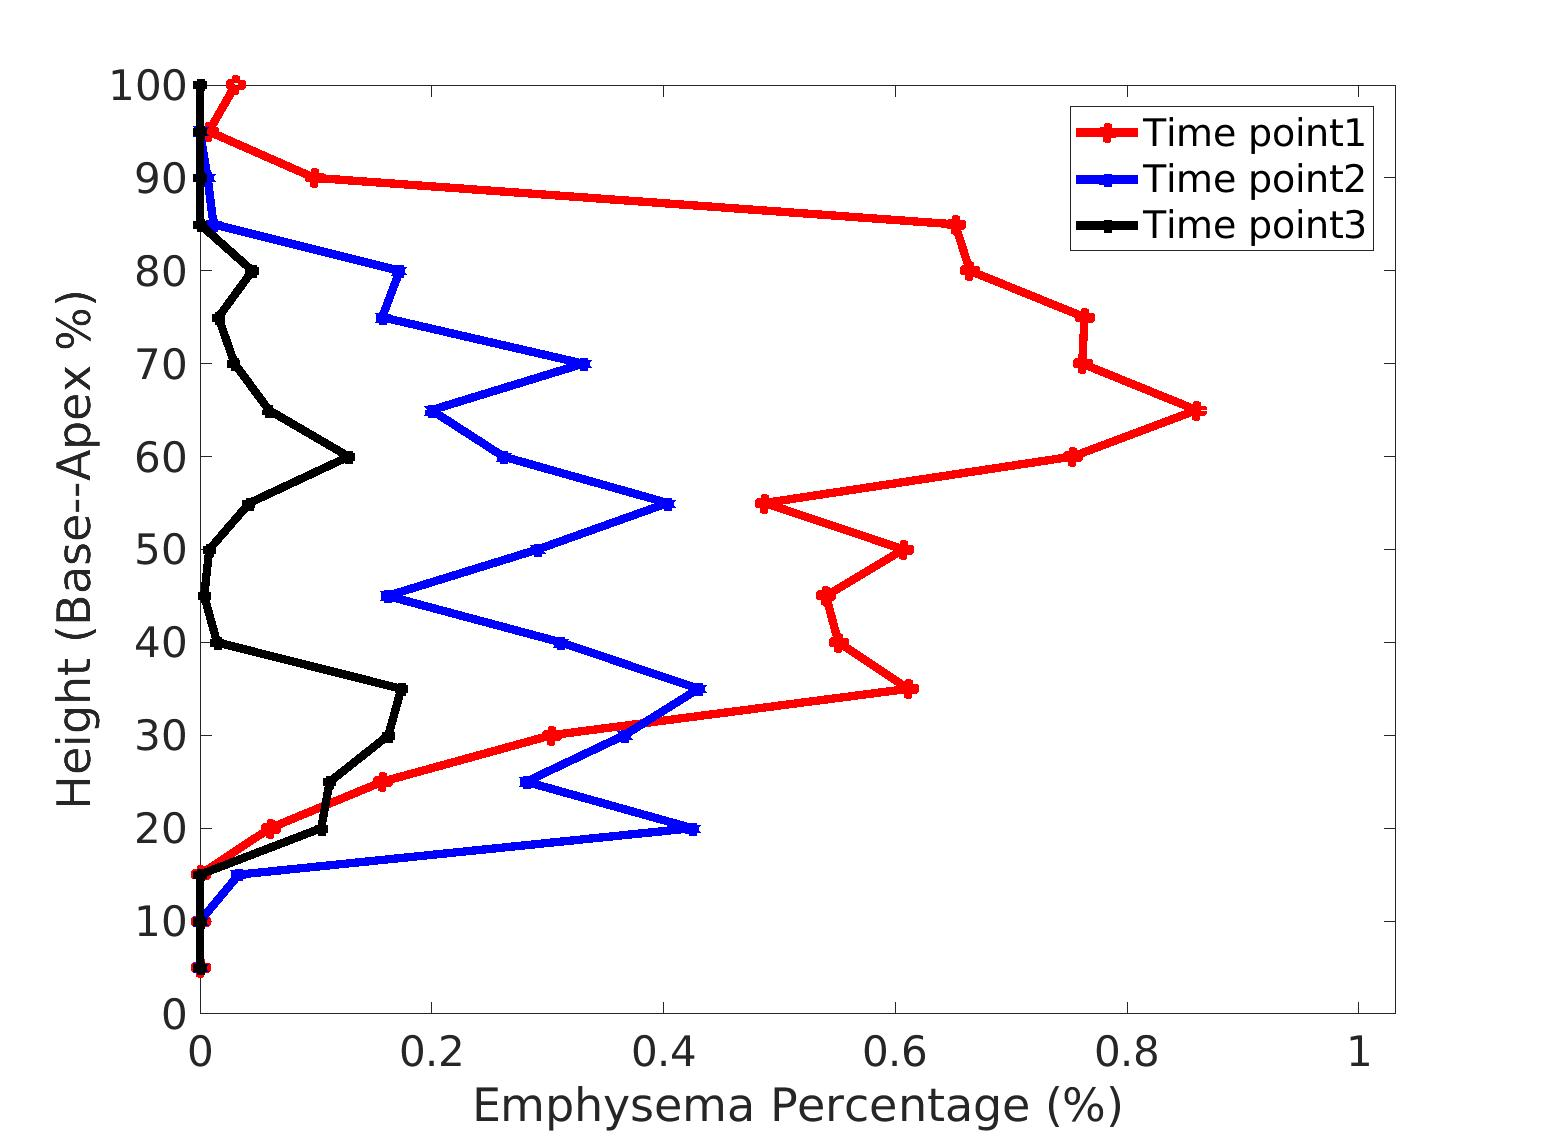
\includegraphics[width=\linewidth,trim={{.0\wd0} {.0\wd0} {.0\wd0} {.0\wd0}},clip]{Appendix/Image_AppexA/BaseToApex/IPF2RightLungEmphysemaDiseaseAgainstHeight.jpg}
  \caption{Right Emphysema}
  \label{fig:IPF2DiseaseAgainstHeight-h}
\end{subfigure}
\caption{Volume percentage of each tissue classification plotted against lung height (cranio-caudal axis) of case IPF2 in left and right lungs over time. The average percentage was calculated within 5\% sections of the lung height from the base to apex. (a) (b) is ground-glass distribution. (c) (d) is reticular distribution. (e) (f) is honeycomb distribution. (g) (h) is emphysema distribution.}
\label{fig:IPF2DiseaseAgainstHeight}
\end{figure}

\begin{figure}[H] 
\centering
\begin{subfigure}{.42\linewidth}% set image scale
  \sbox0{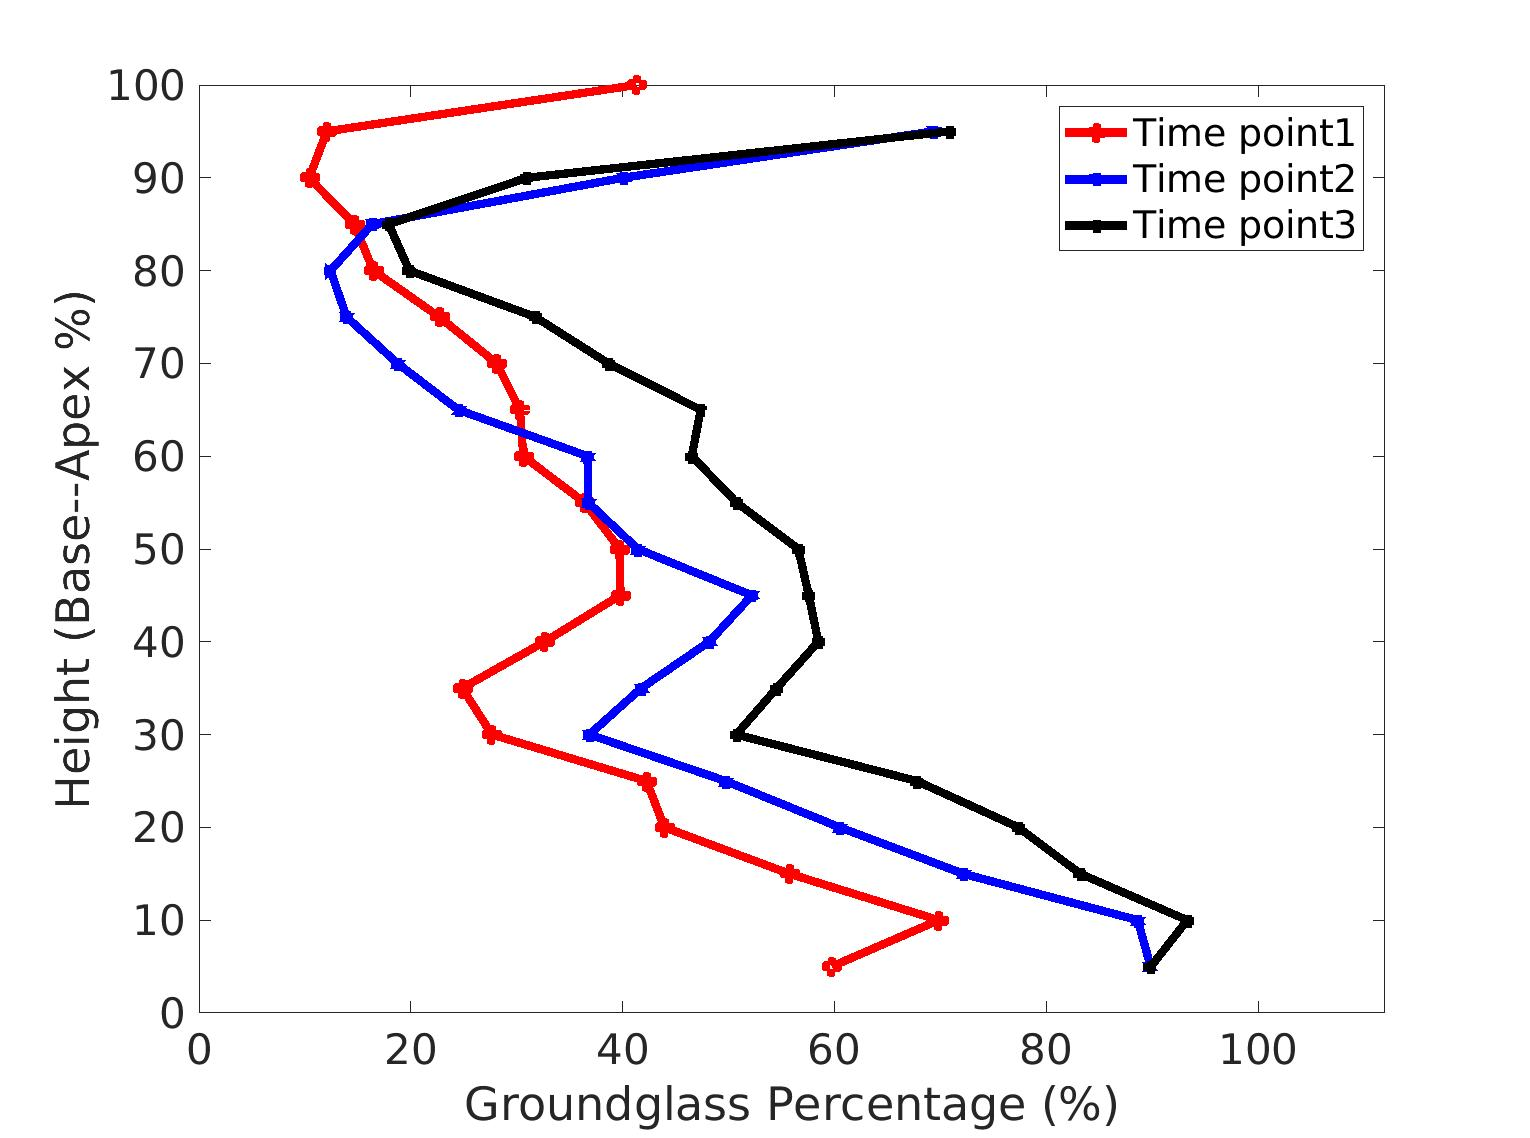
\includegraphics{Appendix/Image_AppexA/BaseToApex/IPF3LeftLungGroundglassDiseaseAgainstHeight.jpg}} 
  %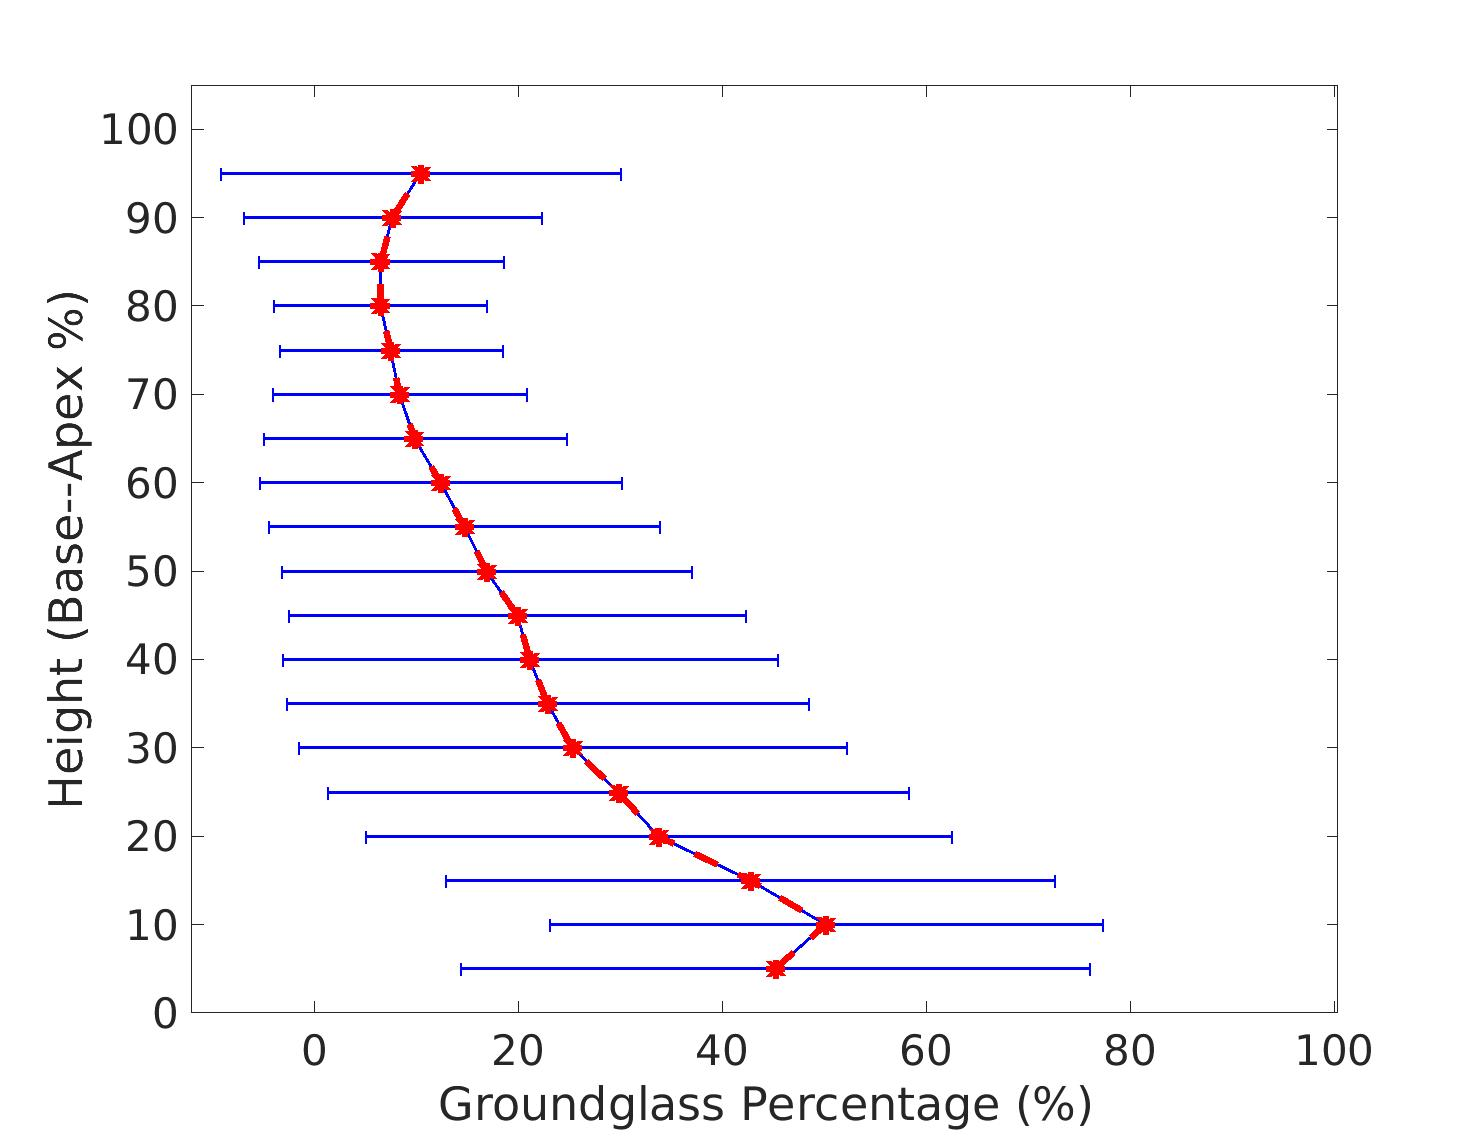
\includegraphics[width=\linewidth,trim={{.0\wd0} {.0\wd0} {.0\wd0} {.0\wd0}},clip]{QuantitativeAnalysis/Image/LeftLungGroundglassDiseaseAgainstHeight.jpg} %trim={<left> <lower> <right> <upper>}, set the cut scale
	\begin{overpic}[width=\linewidth,trim={{.0\wd0} {.0\wd0} {.0\wd0} {.0\wd0}},clip]{Appendix/Image_AppexA/BaseToApex/IPF3LeftLungGroundglassDiseaseAgainstHeight.jpg}
      \put(33,75){\bf{IPF3 left lung}}
  \end{overpic}
  \caption{Left ground-glass}
  \label{fig:IPF3DiseaseAgainstHeight-a} 
\end{subfigure} 
\begin{subfigure}{.42\linewidth}% set image scale
  \sbox0{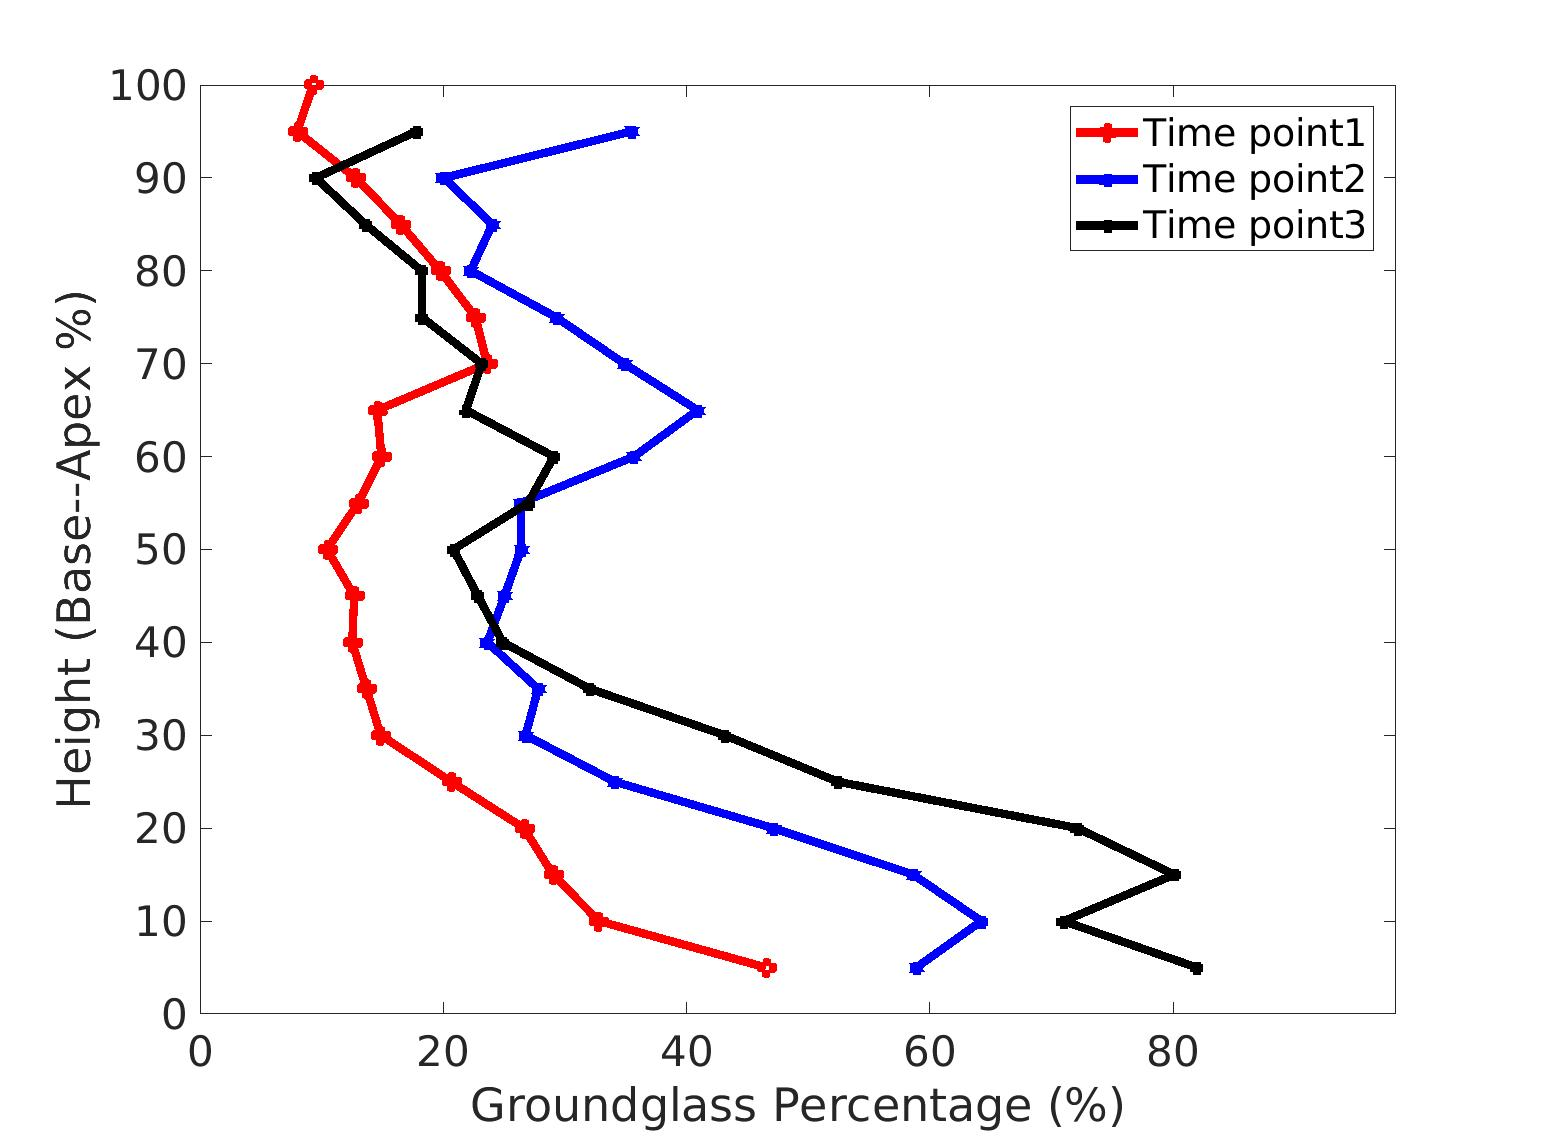
\includegraphics{Appendix/Image_AppexA/BaseToApex/IPF3RightLungGroundglassDiseaseAgainstHeight.jpg}}
  \begin{overpic}[width=\linewidth,trim={{.0\wd0} {.0\wd0} {.0\wd0} {.0\wd0}},clip]{Appendix/Image_AppexA/BaseToApex/IPF3RightLungGroundglassDiseaseAgainstHeight.jpg}
	\put(41,75){\bf{IPF3 right lung}}
  \end{overpic}
  \caption{Right ground-glass}
  \label{fig:IPF3DiseaseAgainstHeight-b}
\end{subfigure}
\begin{subfigure}{.42\linewidth}% set image scale
  \sbox0{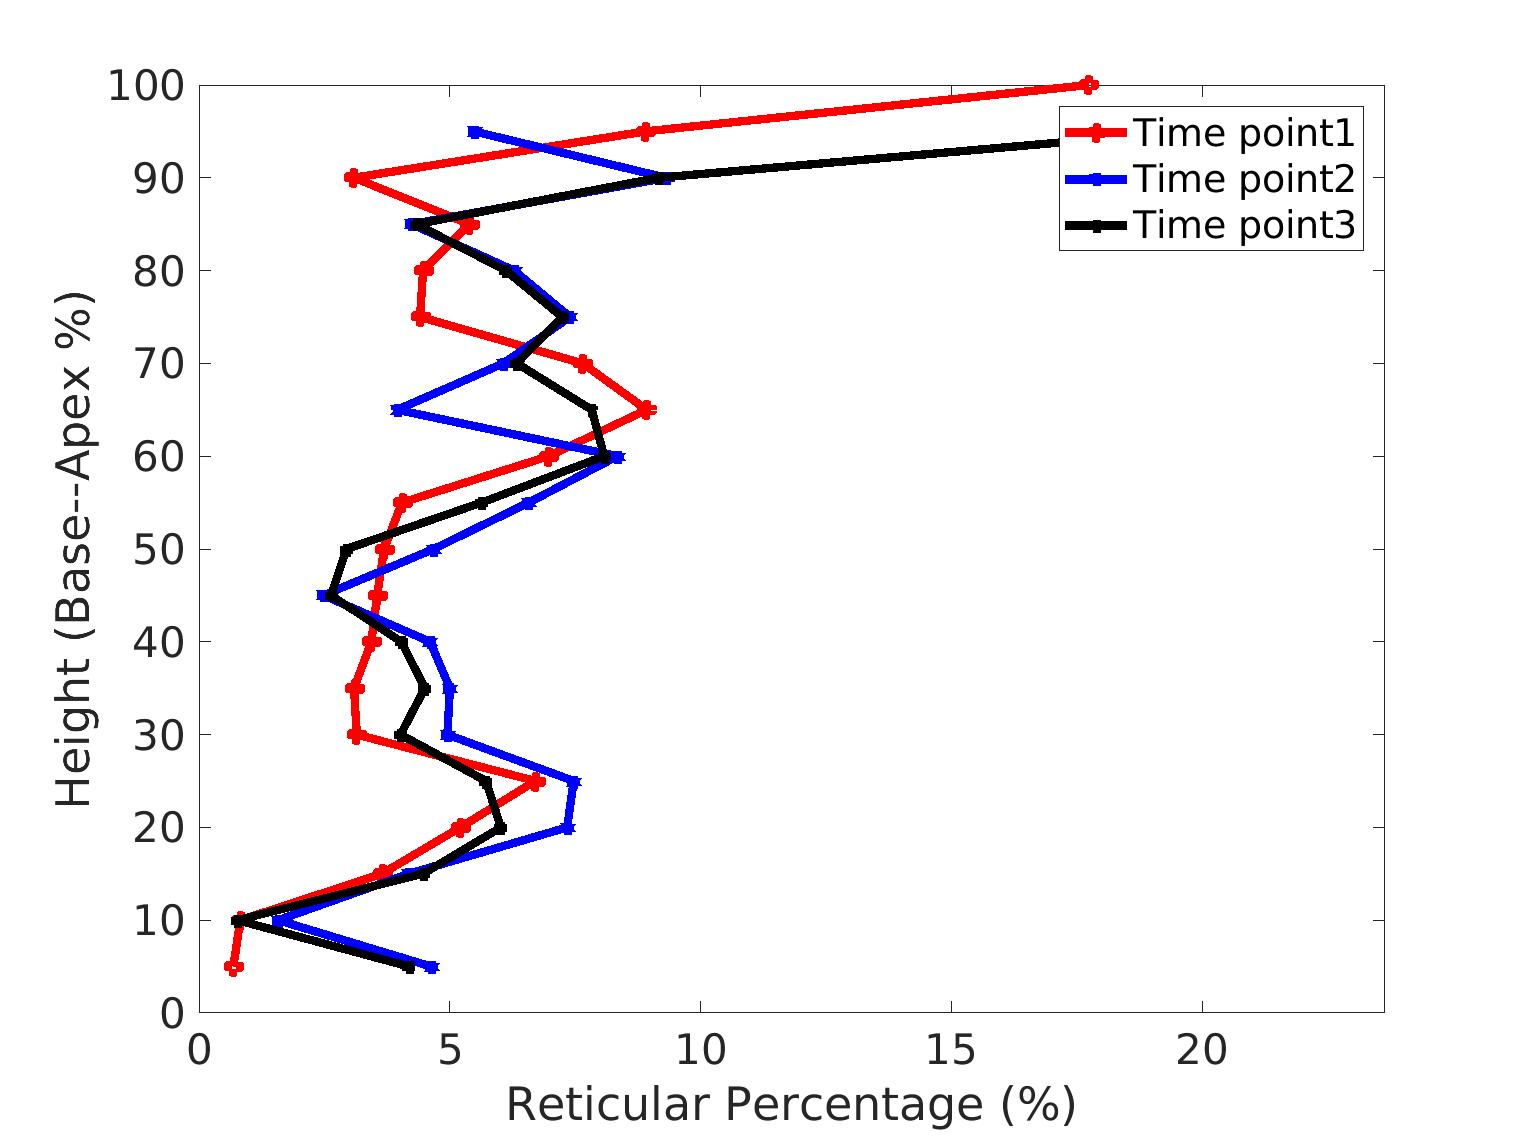
\includegraphics{Appendix/Image_AppexA/BaseToApex/IPF3LeftLungReticularDiseaseAgainstHeight.jpg}} 
  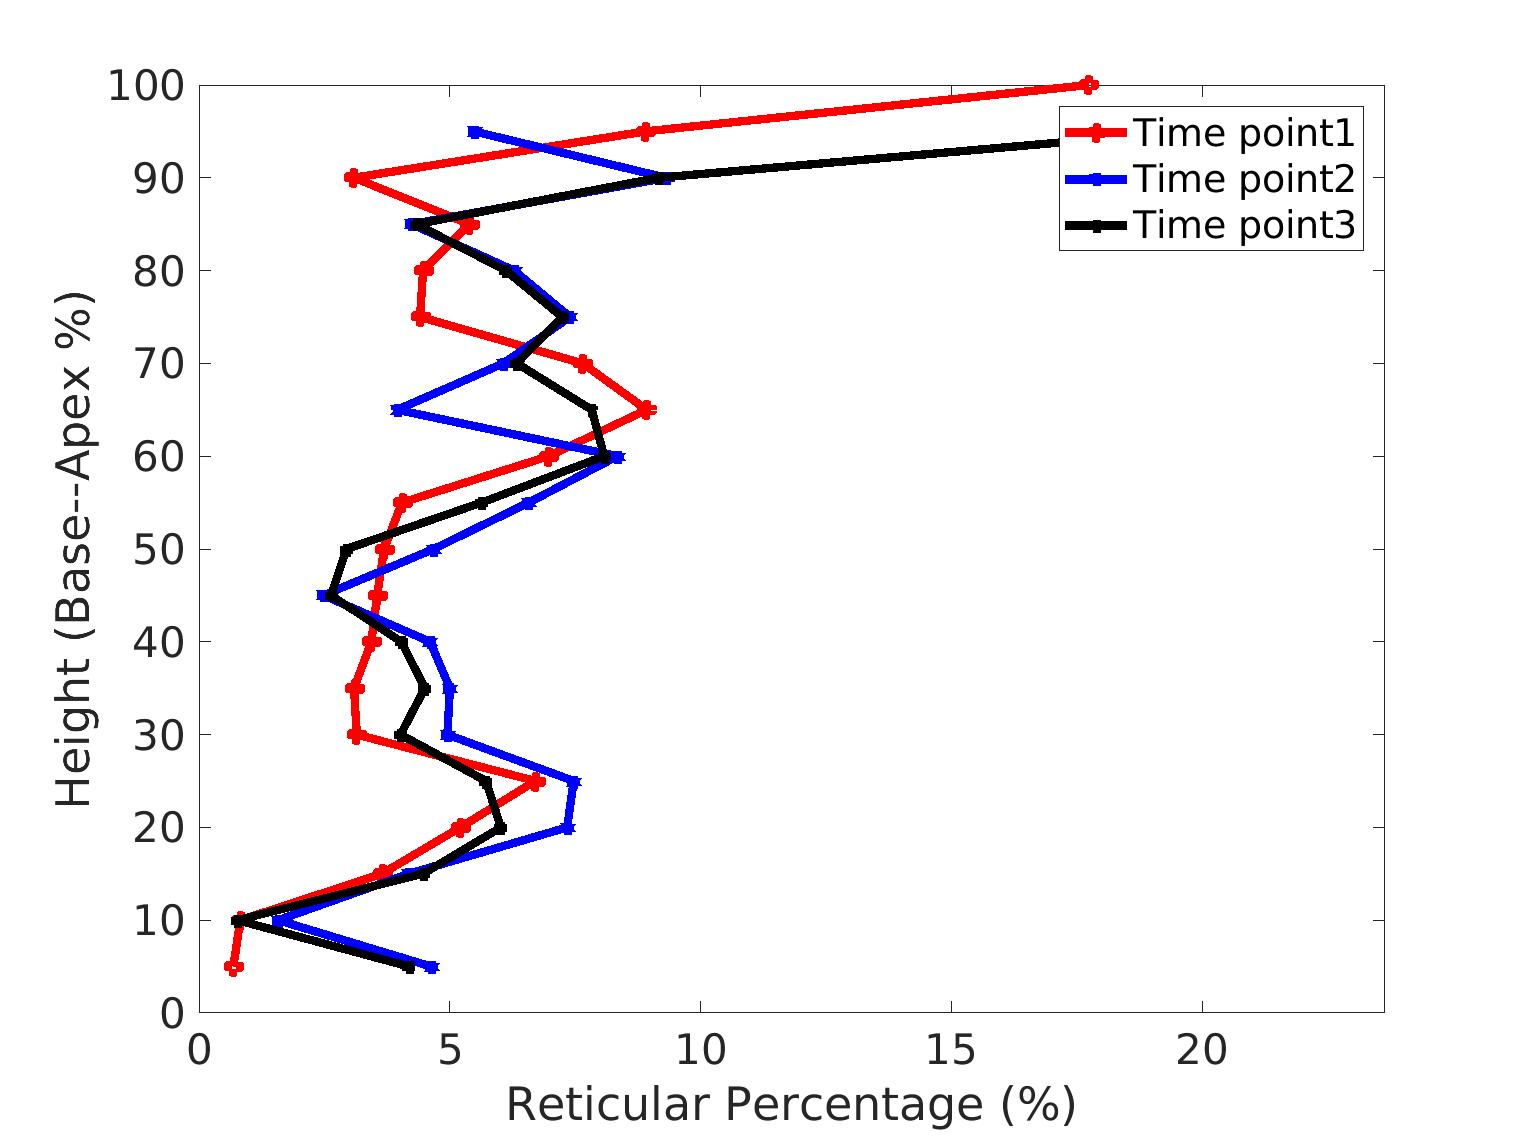
\includegraphics[width=\linewidth,trim={{.0\wd0} {.0\wd0} {.0\wd0} {.0\wd0}},clip]{Appendix/Image_AppexA/BaseToApex/IPF3LeftLungReticularDiseaseAgainstHeight.jpg} %trim={<left> <lower> <right> <upper>}, set the cut scale
  \caption{Left reticular}
  \label{fig:IPF3DiseaseAgainstHeight-c} 
\end{subfigure} 
\begin{subfigure}{.42\linewidth}% set image scale
  \sbox0{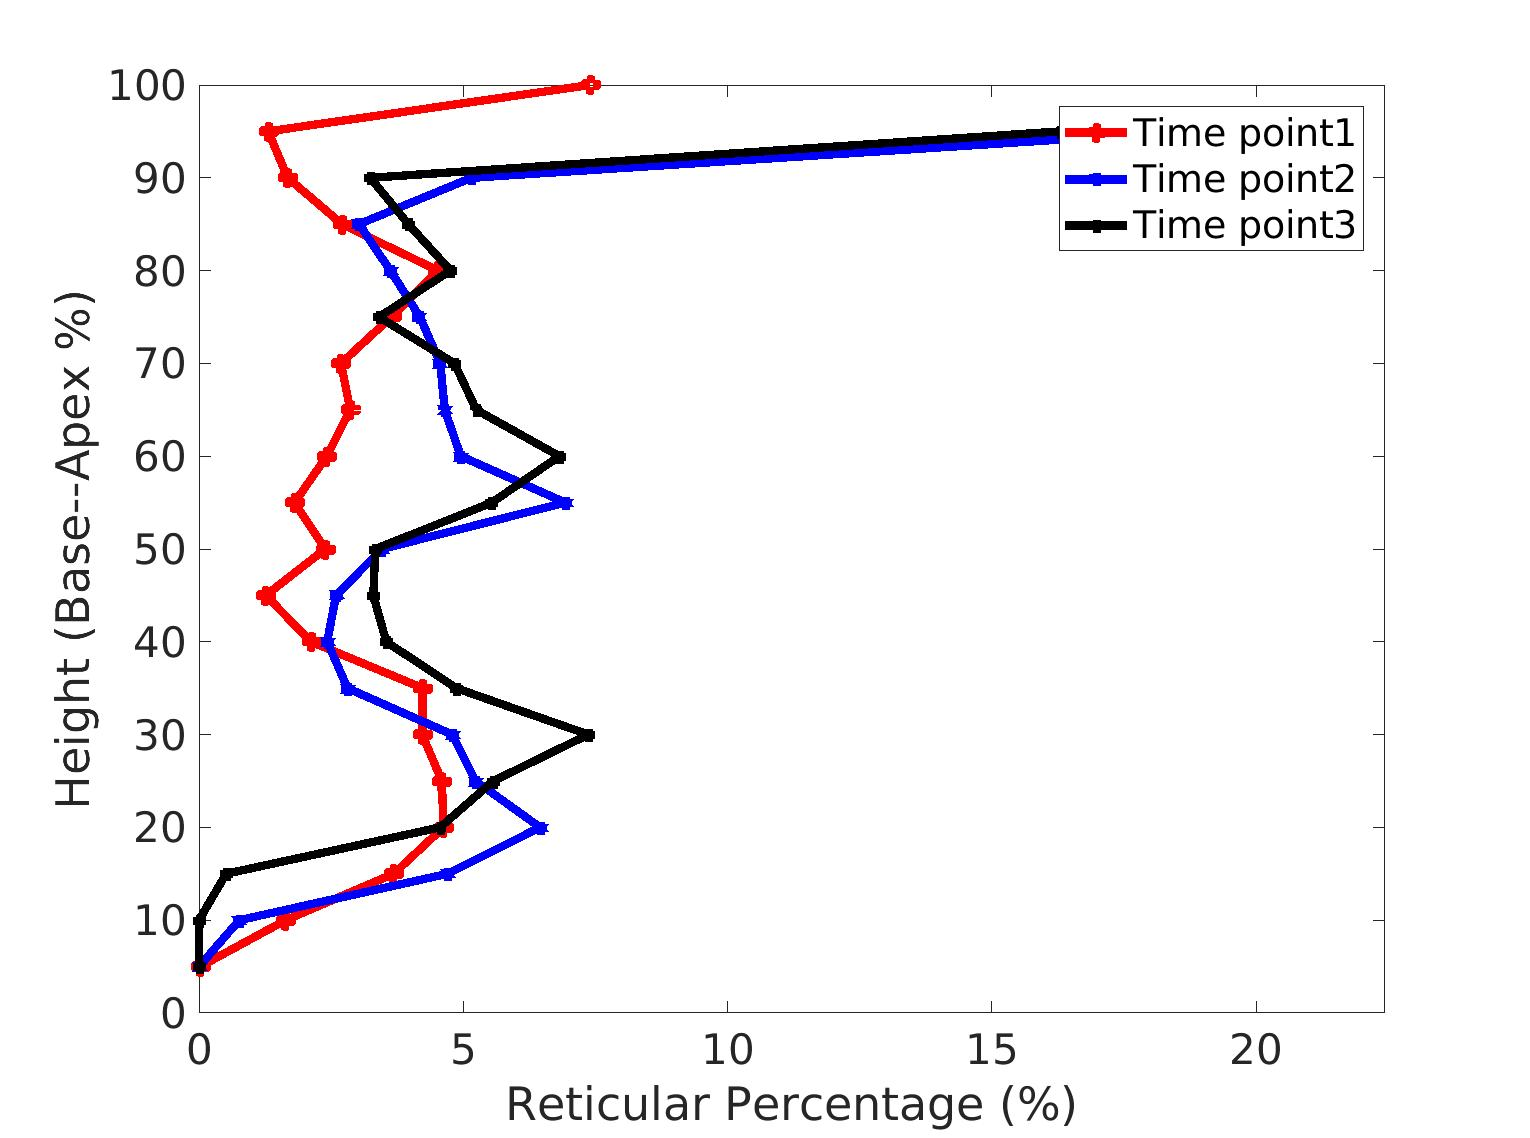
\includegraphics{Appendix/Image_AppexA/BaseToApex/IPF3RightLungReticularDiseaseAgainstHeight.jpg}}
  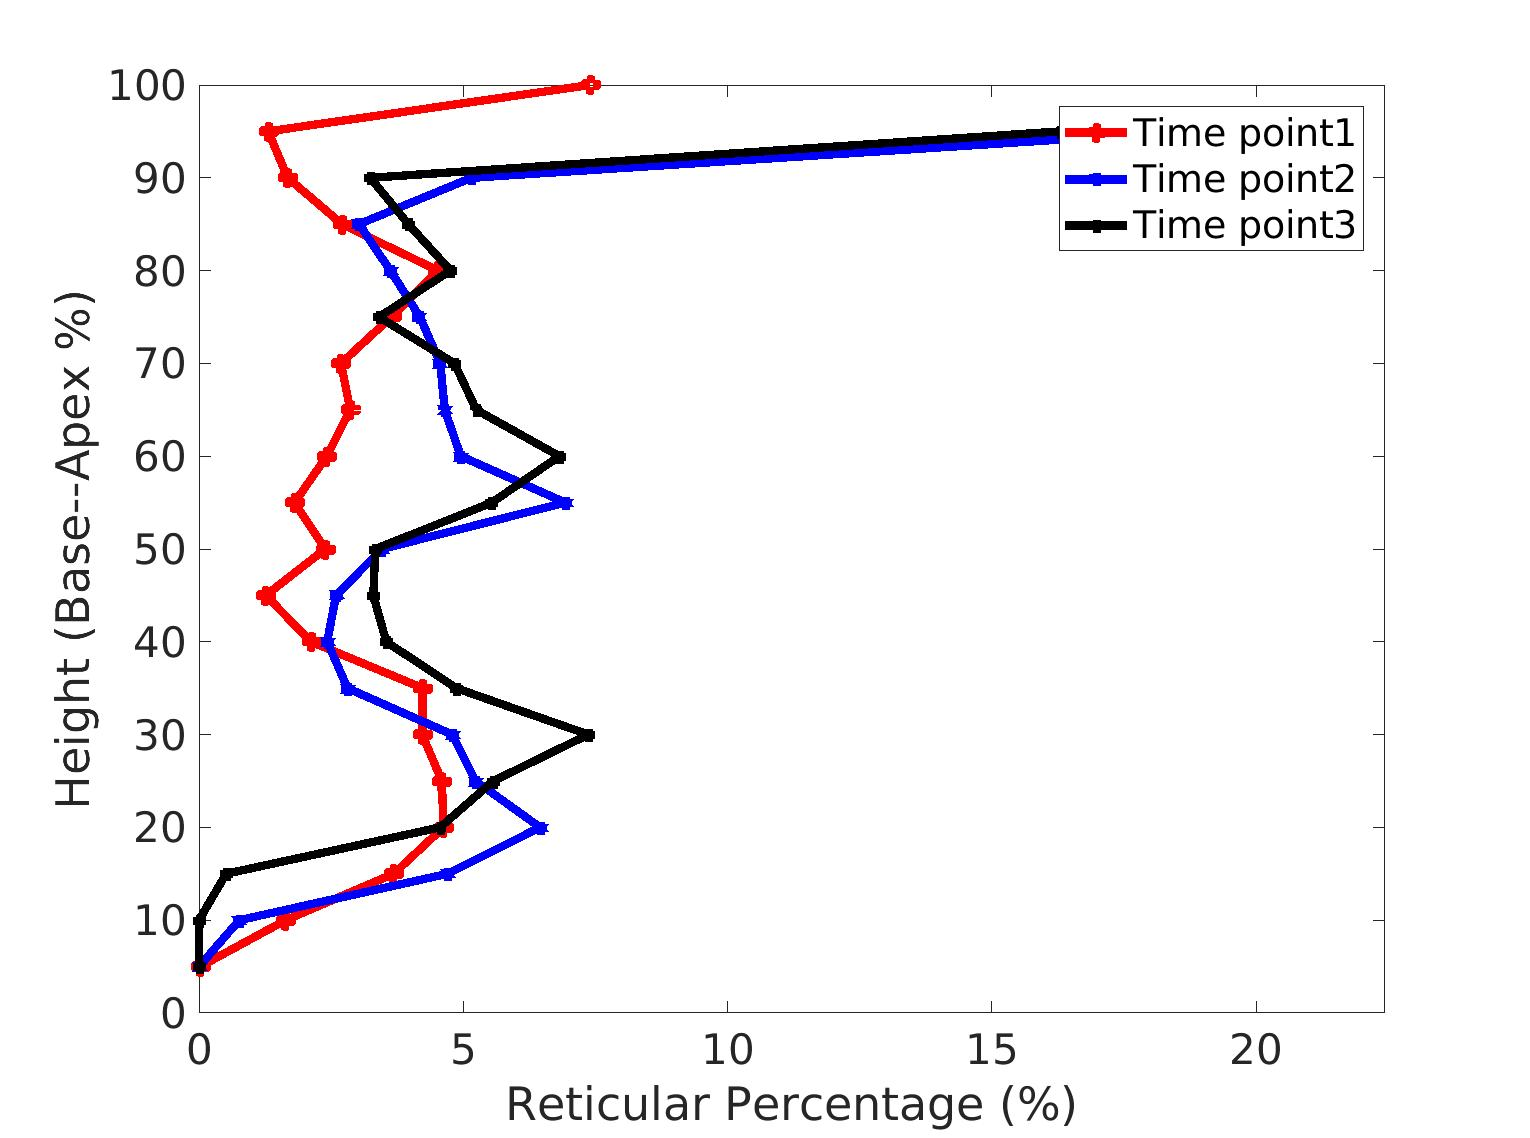
\includegraphics[width=\linewidth,trim={{.0\wd0} {.0\wd0} {.0\wd0} {.0\wd0}},clip]{Appendix/Image_AppexA/BaseToApex/IPF3RightLungReticularDiseaseAgainstHeight.jpg}
  \caption{Right reticular}
  \label{fig:IPF3DiseaseAgainstHeight-d}
\end{subfigure}
\begin{subfigure}{.42\linewidth}% set image scale
  \sbox0{\includegraphics{Appendix/Image_AppexA/BaseToApex/IPF3LeftLungHoneycombDiseaseAgainstHeight.jpg}} 
  \includegraphics[width=\linewidth,trim={{.0\wd0} {.0\wd0} {.0\wd0} {.0\wd0}},clip]{Appendix/Image_AppexA/BaseToApex/IPF3LeftLungHoneycombDiseaseAgainstHeight.jpg} %trim={<left> <lower> <right> <upper>}, set the cut scale
  \caption{Left honeycomb}
  \label{fig:IPF3DiseaseAgainstHeight-e} 
\end{subfigure} 
\begin{subfigure}{.42\linewidth}% set image scale
  \sbox0{\includegraphics{Appendix/Image_AppexA/BaseToApex/IPF3RightLungHoneycombDiseaseAgainstHeight.jpg}}
  \includegraphics[width=\linewidth,trim={{.0\wd0} {.0\wd0} {.0\wd0} {.0\wd0}},clip]{Appendix/Image_AppexA/BaseToApex/IPF3RightLungHoneycombDiseaseAgainstHeight.jpg}
  \caption{Right honeycomb}
  \label{fig:IPF3DiseaseAgainstHeight-f}
\end{subfigure}
\begin{subfigure}{.42\linewidth}% set image scale
  \sbox0{\includegraphics{Appendix/Image_AppexA/BaseToApex/IPF3LeftLungEmphysemaDiseaseAgainstHeight.jpg}} 
  \includegraphics[width=\linewidth,trim={{.0\wd0} {.0\wd0} {.0\wd0} {.0\wd0}},clip]{Appendix/Image_AppexA/BaseToApex/IPF3LeftLungEmphysemaDiseaseAgainstHeight.jpg} %trim={<left> <lower> <right> <upper>}, set the cut scale
  \caption{Left Emphysema}
  \label{fig:IPF3DiseaseAgainstHeight-g} 
\end{subfigure} 
\begin{subfigure}{.42\linewidth}% set image scale
  \sbox0{\includegraphics{Appendix/Image_AppexA/BaseToApex/IPF3RightLungEmphysemaDiseaseAgainstHeight.jpg}}
  \includegraphics[width=\linewidth,trim={{.0\wd0} {.0\wd0} {.0\wd0} {.0\wd0}},clip]{Appendix/Image_AppexA/BaseToApex/IPF3RightLungEmphysemaDiseaseAgainstHeight.jpg}
  \caption{Right Emphysema}
  \label{fig:IPF3DiseaseAgainstHeight-h}
\end{subfigure}
\caption{Volume percentage of each tissue classification plotted against lung height (cranio-caudal axis) of case IPF3 in left and right lungs over time. The average percentage was calculated within 5\% sections of the lung height from the base to apex. (a) (b) is ground-glass distribution. (c) (d) is reticular distribution. (e) (f) is honeycomb distribution. (g) (h) is emphysema distribution.}
\label{fig:IPF3DiseaseAgainstHeight}
\end{figure}

\begin{figure}[H] 
\centering
\begin{subfigure}{.42\linewidth}% set image scale
  \sbox0{\includegraphics{Appendix/Image_AppexA/BaseToApex/IPF5LeftLungGroundglassDiseaseAgainstHeight.jpg}} 
  %\includegraphics[width=\linewidth,trim={{.0\wd0} {.0\wd0} {.0\wd0} {.0\wd0}},clip]{QuantitativeAnalysis/Image/LeftLungGroundglassDiseaseAgainstHeight.jpg} %trim={<left> <lower> <right> <upper>}, set the cut scale
	\begin{overpic}[width=\linewidth,trim={{.0\wd0} {.0\wd0} {.0\wd0} {.0\wd0}},clip]{Appendix/Image_AppexA/BaseToApex/IPF5LeftLungGroundglassDiseaseAgainstHeight.jpg}
      \put(33,75){\bf{IPF5 left lung}}
  \end{overpic}
  \caption{Left ground-glass}
  \label{fig:IPF5DiseaseAgainstHeight-a} 
\end{subfigure} 
\begin{subfigure}{.42\linewidth}% set image scale
  \sbox0{\includegraphics{Appendix/Image_AppexA/BaseToApex/IPF5RightLungGroundglassDiseaseAgainstHeight.jpg}}
  \begin{overpic}[width=\linewidth,trim={{.0\wd0} {.0\wd0} {.0\wd0} {.0\wd0}},clip]{Appendix/Image_AppexA/BaseToApex/IPF5RightLungGroundglassDiseaseAgainstHeight.jpg}
	\put(41,75){\bf{IPF5 right lung}}
  \end{overpic}
  \caption{Right ground-glass}
  \label{fig:IPF5DiseaseAgainstHeight-b}
\end{subfigure}
\begin{subfigure}{.42\linewidth}% set image scale
  \sbox0{\includegraphics{Appendix/Image_AppexA/BaseToApex/IPF5LeftLungReticularDiseaseAgainstHeight.jpg}} 
  \includegraphics[width=\linewidth,trim={{.0\wd0} {.0\wd0} {.0\wd0} {.0\wd0}},clip]{Appendix/Image_AppexA/BaseToApex/IPF5LeftLungReticularDiseaseAgainstHeight.jpg} %trim={<left> <lower> <right> <upper>}, set the cut scale
  \caption{Left reticular}
  \label{fig:IPF5DiseaseAgainstHeight-c} 
\end{subfigure} 
\begin{subfigure}{.42\linewidth}% set image scale
  \sbox0{\includegraphics{Appendix/Image_AppexA/BaseToApex/IPF5RightLungReticularDiseaseAgainstHeight.jpg}}
  \includegraphics[width=\linewidth,trim={{.0\wd0} {.0\wd0} {.0\wd0} {.0\wd0}},clip]{Appendix/Image_AppexA/BaseToApex/IPF5RightLungReticularDiseaseAgainstHeight.jpg}
  \caption{Right reticular}
  \label{fig:IPF5DiseaseAgainstHeight-d}
\end{subfigure}
\begin{subfigure}{.42\linewidth}% set image scale
  \sbox0{\includegraphics{Appendix/Image_AppexA/BaseToApex/IPF5LeftLungHoneycombDiseaseAgainstHeight.jpg}} 
  \includegraphics[width=\linewidth,trim={{.0\wd0} {.0\wd0} {.0\wd0} {.0\wd0}},clip]{Appendix/Image_AppexA/BaseToApex/IPF5LeftLungHoneycombDiseaseAgainstHeight.jpg} %trim={<left> <lower> <right> <upper>}, set the cut scale
  \caption{Left honeycomb}
  \label{fig:IPF5DiseaseAgainstHeight-e} 
\end{subfigure} 
\begin{subfigure}{.42\linewidth}% set image scale
  \sbox0{\includegraphics{Appendix/Image_AppexA/BaseToApex/IPF5RightLungHoneycombDiseaseAgainstHeight.jpg}}
  \includegraphics[width=\linewidth,trim={{.0\wd0} {.0\wd0} {.0\wd0} {.0\wd0}},clip]{Appendix/Image_AppexA/BaseToApex/IPF5RightLungHoneycombDiseaseAgainstHeight.jpg}
  \caption{Right honeycomb}
  \label{fig:IPF5DiseaseAgainstHeight-f}
\end{subfigure}
\begin{subfigure}{.42\linewidth}% set image scale
  \sbox0{\includegraphics{Appendix/Image_AppexA/BaseToApex/IPF5LeftLungEmphysemaDiseaseAgainstHeight.jpg}} 
  \includegraphics[width=\linewidth,trim={{.0\wd0} {.0\wd0} {.0\wd0} {.0\wd0}},clip]{Appendix/Image_AppexA/BaseToApex/IPF5LeftLungEmphysemaDiseaseAgainstHeight.jpg} %trim={<left> <lower> <right> <upper>}, set the cut scale
  \caption{Left Emphysema}
  \label{fig:IPF5DiseaseAgainstHeight-g} 
\end{subfigure} 
\begin{subfigure}{.42\linewidth}% set image scale
  \sbox0{\includegraphics{Appendix/Image_AppexA/BaseToApex/IPF5RightLungEmphysemaDiseaseAgainstHeight.jpg}}
  \includegraphics[width=\linewidth,trim={{.0\wd0} {.0\wd0} {.0\wd0} {.0\wd0}},clip]{Appendix/Image_AppexA/BaseToApex/IPF5RightLungEmphysemaDiseaseAgainstHeight.jpg}
  \caption{Right Emphysema}
  \label{fig:IPF5DiseaseAgainstHeight-h}
\end{subfigure}
\caption{Volume percentage of each tissue classification plotted against lung height (cranio-caudal axis) of case IPF5 in left and right lungs over time. The average percentage was calculated within 5\% sections of the lung height from the base to apex. (a) (b) is ground-glass distribution. (c) (d) is reticular distribution. (e) (f) is honeycomb distribution. (g) (h) is emphysema distribution.}
\label{fig:IPF5DiseaseAgainstHeight}
\end{figure}

\begin{figure}[H] 
\centering
\begin{subfigure}{.42\linewidth}% set image scale
  \sbox0{\includegraphics{Appendix/Image_AppexA/BaseToApex/IPF6LeftLungGroundglassDiseaseAgainstHeight.jpg}} 
  %\includegraphics[width=\linewidth,trim={{.0\wd0} {.0\wd0} {.0\wd0} {.0\wd0}},clip]{QuantitativeAnalysis/Image/LeftLungGroundglassDiseaseAgainstHeight.jpg} %trim={<left> <lower> <right> <upper>}, set the cut scale
	\begin{overpic}[width=\linewidth,trim={{.0\wd0} {.0\wd0} {.0\wd0} {.0\wd0}},clip]{Appendix/Image_AppexA/BaseToApex/IPF6LeftLungGroundglassDiseaseAgainstHeight.jpg}
      \put(33,75){\bf{IPF6 left lung}}
  \end{overpic}
  \caption{Left ground-glass}
  \label{fig:IPF6DiseaseAgainstHeight-a} 
\end{subfigure} 
\begin{subfigure}{.42\linewidth}% set image scale
  \sbox0{\includegraphics{Appendix/Image_AppexA/BaseToApex/IPF6RightLungGroundglassDiseaseAgainstHeight.jpg}}
  \begin{overpic}[width=\linewidth,trim={{.0\wd0} {.0\wd0} {.0\wd0} {.0\wd0}},clip]{Appendix/Image_AppexA/BaseToApex/IPF6RightLungGroundglassDiseaseAgainstHeight.jpg}
	\put(41,75){\bf{IPF6 right lung}}
  \end{overpic}
  \caption{Right ground-glass}
  \label{fig:IPF6DiseaseAgainstHeight-b}
\end{subfigure}
\begin{subfigure}{.42\linewidth}% set image scale
  \sbox0{\includegraphics{Appendix/Image_AppexA/BaseToApex/IPF6LeftLungReticularDiseaseAgainstHeight.jpg}} 
  \includegraphics[width=\linewidth,trim={{.0\wd0} {.0\wd0} {.0\wd0} {.0\wd0}},clip]{Appendix/Image_AppexA/BaseToApex/IPF6LeftLungReticularDiseaseAgainstHeight.jpg} %trim={<left> <lower> <right> <upper>}, set the cut scale
  \caption{Left reticular}
  \label{fig:IPF6DiseaseAgainstHeight-c} 
\end{subfigure} 
\begin{subfigure}{.42\linewidth}% set image scale
  \sbox0{\includegraphics{Appendix/Image_AppexA/BaseToApex/IPF6RightLungReticularDiseaseAgainstHeight.jpg}}
  \includegraphics[width=\linewidth,trim={{.0\wd0} {.0\wd0} {.0\wd0} {.0\wd0}},clip]{Appendix/Image_AppexA/BaseToApex/IPF6RightLungReticularDiseaseAgainstHeight.jpg}
  \caption{Right reticular}
  \label{fig:IPF6DiseaseAgainstHeight-d}
\end{subfigure}
\begin{subfigure}{.42\linewidth}% set image scale
  \sbox0{\includegraphics{Appendix/Image_AppexA/BaseToApex/IPF6LeftLungHoneycombDiseaseAgainstHeight.jpg}} 
  \includegraphics[width=\linewidth,trim={{.0\wd0} {.0\wd0} {.0\wd0} {.0\wd0}},clip]{Appendix/Image_AppexA/BaseToApex/IPF6LeftLungHoneycombDiseaseAgainstHeight.jpg} %trim={<left> <lower> <right> <upper>}, set the cut scale
  \caption{Left honeycomb}
  \label{fig:IPF6DiseaseAgainstHeight-e} 
\end{subfigure} 
\begin{subfigure}{.42\linewidth}% set image scale
  \sbox0{\includegraphics{Appendix/Image_AppexA/BaseToApex/IPF6RightLungHoneycombDiseaseAgainstHeight.jpg}}
  \includegraphics[width=\linewidth,trim={{.0\wd0} {.0\wd0} {.0\wd0} {.0\wd0}},clip]{Appendix/Image_AppexA/BaseToApex/IPF6RightLungHoneycombDiseaseAgainstHeight.jpg}
  \caption{Right honeycomb}
  \label{fig:IPF6DiseaseAgainstHeight-f}
\end{subfigure}
\begin{subfigure}{.42\linewidth}% set image scale
  \sbox0{\includegraphics{Appendix/Image_AppexA/BaseToApex/IPF6LeftLungEmphysemaDiseaseAgainstHeight.jpg}} 
  \includegraphics[width=\linewidth,trim={{.0\wd0} {.0\wd0} {.0\wd0} {.0\wd0}},clip]{Appendix/Image_AppexA/BaseToApex/IPF6LeftLungEmphysemaDiseaseAgainstHeight.jpg} %trim={<left> <lower> <right> <upper>}, set the cut scale
  \caption{Left Emphysema}
  \label{fig:IPF6DiseaseAgainstHeight-g} 
\end{subfigure} 
\begin{subfigure}{.42\linewidth}% set image scale
  \sbox0{\includegraphics{Appendix/Image_AppexA/BaseToApex/IPF6RightLungEmphysemaDiseaseAgainstHeight.jpg}}
  \includegraphics[width=\linewidth,trim={{.0\wd0} {.0\wd0} {.0\wd0} {.0\wd0}},clip]{Appendix/Image_AppexA/BaseToApex/IPF6RightLungEmphysemaDiseaseAgainstHeight.jpg}
  \caption{Right Emphysema}
  \label{fig:IPF6DiseaseAgainstHeight-h}
\end{subfigure}
\caption{Volume percentage of each tissue classification plotted against lung height (cranio-caudal axis) of case IPF6 in left and right lungs over time. The average percentage was calculated within 5\% sections of the lung height from the base to apex. (a) (b) is ground-glass distribution. (c) (d) is reticular distribution. (e) (f) is honeycomb distribution. (g) (h) is emphysema distribution.}
\label{fig:IPF6DiseaseAgainstHeight}
\end{figure}

\begin{figure}[H] 
\centering
\begin{subfigure}{.42\linewidth}% set image scale
  \sbox0{\includegraphics{Appendix/Image_AppexA/BaseToApex/IPF9LeftLungGroundglassDiseaseAgainstHeight.jpg}} 
  %\includegraphics[width=\linewidth,trim={{.0\wd0} {.0\wd0} {.0\wd0} {.0\wd0}},clip]{QuantitativeAnalysis/Image/LeftLungGroundglassDiseaseAgainstHeight.jpg} %trim={<left> <lower> <right> <upper>}, set the cut scale
	\begin{overpic}[width=\linewidth,trim={{.0\wd0} {.0\wd0} {.0\wd0} {.0\wd0}},clip]{Appendix/Image_AppexA/BaseToApex/IPF9LeftLungGroundglassDiseaseAgainstHeight.jpg}
      \put(33,75){\bf{IPF9 left lung}}
  \end{overpic}
  \caption{Left ground-glass}
  \label{fig:IPF9DiseaseAgainstHeight-a} 
\end{subfigure} 
\begin{subfigure}{.42\linewidth}% set image scale
  \sbox0{\includegraphics{Appendix/Image_AppexA/BaseToApex/IPF9RightLungGroundglassDiseaseAgainstHeight.jpg}}
  \begin{overpic}[width=\linewidth,trim={{.0\wd0} {.0\wd0} {.0\wd0} {.0\wd0}},clip]{Appendix/Image_AppexA/BaseToApex/IPF9RightLungGroundglassDiseaseAgainstHeight.jpg}
	\put(41,75){\bf{IPF9 right lung}}
  \end{overpic}
  \caption{Right ground-glass}
  \label{fig:IPF9DiseaseAgainstHeight-b}
\end{subfigure}
\begin{subfigure}{.42\linewidth}% set image scale
  \sbox0{\includegraphics{Appendix/Image_AppexA/BaseToApex/IPF9LeftLungReticularDiseaseAgainstHeight.jpg}} 
  \includegraphics[width=\linewidth,trim={{.0\wd0} {.0\wd0} {.0\wd0} {.0\wd0}},clip]{Appendix/Image_AppexA/BaseToApex/IPF9LeftLungReticularDiseaseAgainstHeight.jpg} %trim={<left> <lower> <right> <upper>}, set the cut scale
  \caption{Left reticular}
  \label{fig:IPF9DiseaseAgainstHeight-c} 
\end{subfigure} 
\begin{subfigure}{.42\linewidth}% set image scale
  \sbox0{\includegraphics{Appendix/Image_AppexA/BaseToApex/IPF9RightLungReticularDiseaseAgainstHeight.jpg}}
  \includegraphics[width=\linewidth,trim={{.0\wd0} {.0\wd0} {.0\wd0} {.0\wd0}},clip]{Appendix/Image_AppexA/BaseToApex/IPF9RightLungReticularDiseaseAgainstHeight.jpg}
  \caption{Right reticular}
  \label{fig:IPF9DiseaseAgainstHeight-d}
\end{subfigure}
\begin{subfigure}{.42\linewidth}% set image scale
  \sbox0{\includegraphics{Appendix/Image_AppexA/BaseToApex/IPF9LeftLungHoneycombDiseaseAgainstHeight.jpg}} 
  \includegraphics[width=\linewidth,trim={{.0\wd0} {.0\wd0} {.0\wd0} {.0\wd0}},clip]{Appendix/Image_AppexA/BaseToApex/IPF9LeftLungHoneycombDiseaseAgainstHeight.jpg} %trim={<left> <lower> <right> <upper>}, set the cut scale
  \caption{Left honeycomb}
  \label{fig:IPF9DiseaseAgainstHeight-e} 
\end{subfigure} 
\begin{subfigure}{.42\linewidth}% set image scale
  \sbox0{\includegraphics{Appendix/Image_AppexA/BaseToApex/IPF9RightLungHoneycombDiseaseAgainstHeight.jpg}}
  \includegraphics[width=\linewidth,trim={{.0\wd0} {.0\wd0} {.0\wd0} {.0\wd0}},clip]{Appendix/Image_AppexA/BaseToApex/IPF9RightLungHoneycombDiseaseAgainstHeight.jpg}
  \caption{Right honeycomb}
  \label{fig:IPF9DiseaseAgainstHeight-f}
\end{subfigure}
\begin{subfigure}{.42\linewidth}% set image scale
  \sbox0{\includegraphics{Appendix/Image_AppexA/BaseToApex/IPF9LeftLungEmphysemaDiseaseAgainstHeight.jpg}} 
  \includegraphics[width=\linewidth,trim={{.0\wd0} {.0\wd0} {.0\wd0} {.0\wd0}},clip]{Appendix/Image_AppexA/BaseToApex/IPF9LeftLungEmphysemaDiseaseAgainstHeight.jpg} %trim={<left> <lower> <right> <upper>}, set the cut scale
  \caption{Left Emphysema}
  \label{fig:IPF9DiseaseAgainstHeight-g} 
\end{subfigure} 
\begin{subfigure}{.42\linewidth}% set image scale
  \sbox0{\includegraphics{Appendix/Image_AppexA/BaseToApex/IPF9RightLungEmphysemaDiseaseAgainstHeight.jpg}}
  \includegraphics[width=\linewidth,trim={{.0\wd0} {.0\wd0} {.0\wd0} {.0\wd0}},clip]{Appendix/Image_AppexA/BaseToApex/IPF9RightLungEmphysemaDiseaseAgainstHeight.jpg}
  \caption{Right Emphysema}
  \label{fig:IPF9DiseaseAgainstHeight-h}
\end{subfigure}
\caption{Volume percentage of each tissue classification plotted against lung height (cranio-caudal axis) of case IPF9 in left and right lungs over time. The average percentage was calculated within 5\% sections of the lung height from the base to apex. (a) (b) is ground-glass distribution. (c) (d) is reticular distribution. (e) (f) is honeycomb distribution. (g) (h) is emphysema distribution.}
\label{fig:IPF9DiseaseAgainstHeight}
\end{figure}

\begin{figure}[H] 
\centering
\begin{subfigure}{.42\linewidth}% set image scale
  \sbox0{\includegraphics{Appendix/Image_AppexA/BaseToApex/IPF10LeftLungGroundglassDiseaseAgainstHeight.jpg}} 
  %\includegraphics[width=\linewidth,trim={{.0\wd0} {.0\wd0} {.0\wd0} {.0\wd0}},clip]{QuantitativeAnalysis/Image/LeftLungGroundglassDiseaseAgainstHeight.jpg} %trim={<left> <lower> <right> <upper>}, set the cut scale
	\begin{overpic}[width=\linewidth,trim={{.0\wd0} {.0\wd0} {.0\wd0} {.0\wd0}},clip]{Appendix/Image_AppexA/BaseToApex/IPF10LeftLungGroundglassDiseaseAgainstHeight.jpg}
      \put(33,75){\bf{IPF10 left lung}}
  \end{overpic}
  \caption{Left ground-glass}
  \label{fig:IPF10DiseaseAgainstHeight-a} 
\end{subfigure} 
\begin{subfigure}{.42\linewidth}% set image scale
  \sbox0{\includegraphics{Appendix/Image_AppexA/BaseToApex/IPF10RightLungGroundglassDiseaseAgainstHeight.jpg}}
  \begin{overpic}[width=\linewidth,trim={{.0\wd0} {.0\wd0} {.0\wd0} {.0\wd0}},clip]{Appendix/Image_AppexA/BaseToApex/IPF10RightLungGroundglassDiseaseAgainstHeight.jpg}
	\put(41,75){\bf{IPF10 right lung}}
  \end{overpic}
  \caption{Right ground-glass}
  \label{fig:IPF10DiseaseAgainstHeight-b}
\end{subfigure}
\begin{subfigure}{.42\linewidth}% set image scale
  \sbox0{\includegraphics{Appendix/Image_AppexA/BaseToApex/IPF10LeftLungReticularDiseaseAgainstHeight.jpg}} 
  \includegraphics[width=\linewidth,trim={{.0\wd0} {.0\wd0} {.0\wd0} {.0\wd0}},clip]{Appendix/Image_AppexA/BaseToApex/IPF10LeftLungReticularDiseaseAgainstHeight.jpg} %trim={<left> <lower> <right> <upper>}, set the cut scale
  \caption{Left reticular}
  \label{fig:IPF10DiseaseAgainstHeight-c} 
\end{subfigure} 
\begin{subfigure}{.42\linewidth}% set image scale
  \sbox0{\includegraphics{Appendix/Image_AppexA/BaseToApex/IPF10RightLungReticularDiseaseAgainstHeight.jpg}}
  \includegraphics[width=\linewidth,trim={{.0\wd0} {.0\wd0} {.0\wd0} {.0\wd0}},clip]{Appendix/Image_AppexA/BaseToApex/IPF10RightLungReticularDiseaseAgainstHeight.jpg}
  \caption{Right reticular}
  \label{fig:IPF10DiseaseAgainstHeight-d}
\end{subfigure}
\begin{subfigure}{.42\linewidth}% set image scale
  \sbox0{\includegraphics{Appendix/Image_AppexA/BaseToApex/IPF10LeftLungHoneycombDiseaseAgainstHeight.jpg}} 
  \includegraphics[width=\linewidth,trim={{.0\wd0} {.0\wd0} {.0\wd0} {.0\wd0}},clip]{Appendix/Image_AppexA/BaseToApex/IPF10LeftLungHoneycombDiseaseAgainstHeight.jpg} %trim={<left> <lower> <right> <upper>}, set the cut scale
  \caption{Left honeycomb}
  \label{fig:IPF10DiseaseAgainstHeight-e} 
\end{subfigure} 
\begin{subfigure}{.42\linewidth}% set image scale
  \sbox0{\includegraphics{Appendix/Image_AppexA/BaseToApex/IPF10RightLungHoneycombDiseaseAgainstHeight.jpg}}
  \includegraphics[width=\linewidth,trim={{.0\wd0} {.0\wd0} {.0\wd0} {.0\wd0}},clip]{Appendix/Image_AppexA/BaseToApex/IPF10RightLungHoneycombDiseaseAgainstHeight.jpg}
  \caption{Right honeycomb}
  \label{fig:IPF10DiseaseAgainstHeight-f}
\end{subfigure}
\begin{subfigure}{.42\linewidth}% set image scale
  \sbox0{\includegraphics{Appendix/Image_AppexA/BaseToApex/IPF10LeftLungEmphysemaDiseaseAgainstHeight.jpg}} 
  \includegraphics[width=\linewidth,trim={{.0\wd0} {.0\wd0} {.0\wd0} {.0\wd0}},clip]{Appendix/Image_AppexA/BaseToApex/IPF10LeftLungEmphysemaDiseaseAgainstHeight.jpg} %trim={<left> <lower> <right> <upper>}, set the cut scale
  \caption{Left Emphysema}
  \label{fig:IPF10DiseaseAgainstHeight-g} 
\end{subfigure} 
\begin{subfigure}{.42\linewidth}% set image scale
  \sbox0{\includegraphics{Appendix/Image_AppexA/BaseToApex/IPF10RightLungEmphysemaDiseaseAgainstHeight.jpg}}
  \includegraphics[width=\linewidth,trim={{.0\wd0} {.0\wd0} {.0\wd0} {.0\wd0}},clip]{Appendix/Image_AppexA/BaseToApex/IPF10RightLungEmphysemaDiseaseAgainstHeight.jpg}
  \caption{Right Emphysema}
  \label{fig:IPF10DiseaseAgainstHeight-h}
\end{subfigure}
\caption{Volume percentage of each tissue classification plotted against lung height (cranio-caudal axis) of case IPF10 in left and right lungs over time. The average percentage was calculated within 5\% sections of the lung height from the base to apex. (a) (b) is ground-glass distribution. (c) (d) is reticular distribution. (e) (f) is honeycomb distribution. (g) (h) is emphysema distribution.}
\label{fig:IPF10DiseaseAgainstHeight}
\end{figure}

\begin{figure}[H] 
\centering
\begin{subfigure}{.42\linewidth}% set image scale
  \sbox0{\includegraphics{Appendix/Image_AppexA/BaseToApex/IPF13LeftLungGroundglassDiseaseAgainstHeight.jpg}} 
  %\includegraphics[width=\linewidth,trim={{.0\wd0} {.0\wd0} {.0\wd0} {.0\wd0}},clip]{QuantitativeAnalysis/Image/LeftLungGroundglassDiseaseAgainstHeight.jpg} %trim={<left> <lower> <right> <upper>}, set the cut scale
	\begin{overpic}[width=\linewidth,trim={{.0\wd0} {.0\wd0} {.0\wd0} {.0\wd0}},clip]{Appendix/Image_AppexA/BaseToApex/IPF13LeftLungGroundglassDiseaseAgainstHeight.jpg}
      \put(33,75){\bf{IPF13 left lung}}
  \end{overpic}
  \caption{Left ground-glass}
  \label{fig:IPF13DiseaseAgainstHeight-a} 
\end{subfigure} 
\begin{subfigure}{.42\linewidth}% set image scale
  \sbox0{\includegraphics{Appendix/Image_AppexA/BaseToApex/IPF13RightLungGroundglassDiseaseAgainstHeight.jpg}}
  \begin{overpic}[width=\linewidth,trim={{.0\wd0} {.0\wd0} {.0\wd0} {.0\wd0}},clip]{Appendix/Image_AppexA/BaseToApex/IPF13RightLungGroundglassDiseaseAgainstHeight.jpg}
	\put(41,75){\bf{IPF13 right lung}}
  \end{overpic}
  \caption{Right ground-glass}
  \label{fig:IPF13DiseaseAgainstHeight-b}
\end{subfigure}
\begin{subfigure}{.42\linewidth}% set image scale
  \sbox0{\includegraphics{Appendix/Image_AppexA/BaseToApex/IPF13LeftLungReticularDiseaseAgainstHeight.jpg}} 
  \includegraphics[width=\linewidth,trim={{.0\wd0} {.0\wd0} {.0\wd0} {.0\wd0}},clip]{Appendix/Image_AppexA/BaseToApex/IPF13LeftLungReticularDiseaseAgainstHeight.jpg} %trim={<left> <lower> <right> <upper>}, set the cut scale
  \caption{Left reticular}
  \label{fig:IPF13DiseaseAgainstHeight-c} 
\end{subfigure} 
\begin{subfigure}{.42\linewidth}% set image scale
  \sbox0{\includegraphics{Appendix/Image_AppexA/BaseToApex/IPF13RightLungReticularDiseaseAgainstHeight.jpg}}
  \includegraphics[width=\linewidth,trim={{.0\wd0} {.0\wd0} {.0\wd0} {.0\wd0}},clip]{Appendix/Image_AppexA/BaseToApex/IPF13RightLungReticularDiseaseAgainstHeight.jpg}
  \caption{Right reticular}
  \label{fig:IPF13DiseaseAgainstHeight-d}
\end{subfigure}
\begin{subfigure}{.42\linewidth}% set image scale
  \sbox0{\includegraphics{Appendix/Image_AppexA/BaseToApex/IPF13LeftLungHoneycombDiseaseAgainstHeight.jpg}} 
  \includegraphics[width=\linewidth,trim={{.0\wd0} {.0\wd0} {.0\wd0} {.0\wd0}},clip]{Appendix/Image_AppexA/BaseToApex/IPF13LeftLungHoneycombDiseaseAgainstHeight.jpg} %trim={<left> <lower> <right> <upper>}, set the cut scale
  \caption{Left honeycomb}
  \label{fig:IPF13DiseaseAgainstHeight-e} 
\end{subfigure} 
\begin{subfigure}{.42\linewidth}% set image scale
  \sbox0{\includegraphics{Appendix/Image_AppexA/BaseToApex/IPF13RightLungHoneycombDiseaseAgainstHeight.jpg}}
  \includegraphics[width=\linewidth,trim={{.0\wd0} {.0\wd0} {.0\wd0} {.0\wd0}},clip]{Appendix/Image_AppexA/BaseToApex/IPF13RightLungHoneycombDiseaseAgainstHeight.jpg}
  \caption{Right honeycomb}
  \label{fig:IPF13DiseaseAgainstHeight-f}
\end{subfigure}
\begin{subfigure}{.42\linewidth}% set image scale
  \sbox0{\includegraphics{Appendix/Image_AppexA/BaseToApex/IPF13LeftLungEmphysemaDiseaseAgainstHeight.jpg}} 
  \includegraphics[width=\linewidth,trim={{.0\wd0} {.0\wd0} {.0\wd0} {.0\wd0}},clip]{Appendix/Image_AppexA/BaseToApex/IPF13LeftLungEmphysemaDiseaseAgainstHeight.jpg} %trim={<left> <lower> <right> <upper>}, set the cut scale
  \caption{Left Emphysema}
  \label{fig:IPF13DiseaseAgainstHeight-g} 
\end{subfigure} 
\begin{subfigure}{.42\linewidth}% set image scale
  \sbox0{\includegraphics{Appendix/Image_AppexA/BaseToApex/IPF13RightLungEmphysemaDiseaseAgainstHeight.jpg}}
  \includegraphics[width=\linewidth,trim={{.0\wd0} {.0\wd0} {.0\wd0} {.0\wd0}},clip]{Appendix/Image_AppexA/BaseToApex/IPF13RightLungEmphysemaDiseaseAgainstHeight.jpg}
  \caption{Right Emphysema}
  \label{fig:IPF13DiseaseAgainstHeight-h}
\end{subfigure}
\caption{Volume percentage of each tissue classification plotted against lung height (cranio-caudal axis) of case IPF13 in left and right lungs over time. The average percentage was calculated within 5\% sections of the lung height from the base to apex. (a) (b) is ground-glass distribution. (c) (d) is reticular distribution. (e) (f) is honeycomb distribution. (g) (h) is emphysema distribution.}
\label{fig:IPF13DiseaseAgainstHeight}
\end{figure}

\begin{figure}[H] 
\centering
\begin{subfigure}{.42\linewidth}% set image scale
  \sbox0{\includegraphics{Appendix/Image_AppexA/BaseToApex/IPF14LeftLungGroundglassDiseaseAgainstHeight.jpg}} 
  %\includegraphics[width=\linewidth,trim={{.0\wd0} {.0\wd0} {.0\wd0} {.0\wd0}},clip]{QuantitativeAnalysis/Image/LeftLungGroundglassDiseaseAgainstHeight.jpg} %trim={<left> <lower> <right> <upper>}, set the cut scale
	\begin{overpic}[width=\linewidth,trim={{.0\wd0} {.0\wd0} {.0\wd0} {.0\wd0}},clip]{Appendix/Image_AppexA/BaseToApex/IPF14LeftLungGroundglassDiseaseAgainstHeight.jpg}
      \put(33,75){\bf{IPF14 left lung}}
  \end{overpic}
  \caption{Left ground-glass}
  \label{fig:IPF14DiseaseAgainstHeight-a} 
\end{subfigure} 
\begin{subfigure}{.42\linewidth}% set image scale
  \sbox0{\includegraphics{Appendix/Image_AppexA/BaseToApex/IPF14RightLungGroundglassDiseaseAgainstHeight.jpg}}
  \begin{overpic}[width=\linewidth,trim={{.0\wd0} {.0\wd0} {.0\wd0} {.0\wd0}},clip]{Appendix/Image_AppexA/BaseToApex/IPF14RightLungGroundglassDiseaseAgainstHeight.jpg}
	\put(41,75){\bf{IPF14 right lung}}
  \end{overpic}
  \caption{Right ground-glass}
  \label{fig:IPF14DiseaseAgainstHeight-b}
\end{subfigure}
\begin{subfigure}{.42\linewidth}% set image scale
  \sbox0{\includegraphics{Appendix/Image_AppexA/BaseToApex/IPF14LeftLungReticularDiseaseAgainstHeight.jpg}} 
  \includegraphics[width=\linewidth,trim={{.0\wd0} {.0\wd0} {.0\wd0} {.0\wd0}},clip]{Appendix/Image_AppexA/BaseToApex/IPF14LeftLungReticularDiseaseAgainstHeight.jpg} %trim={<left> <lower> <right> <upper>}, set the cut scale
  \caption{Left reticular}
  \label{fig:IPF14DiseaseAgainstHeight-c} 
\end{subfigure} 
\begin{subfigure}{.42\linewidth}% set image scale
  \sbox0{\includegraphics{Appendix/Image_AppexA/BaseToApex/IPF14RightLungReticularDiseaseAgainstHeight.jpg}}
  \includegraphics[width=\linewidth,trim={{.0\wd0} {.0\wd0} {.0\wd0} {.0\wd0}},clip]{Appendix/Image_AppexA/BaseToApex/IPF14RightLungReticularDiseaseAgainstHeight.jpg}
  \caption{Right reticular}
  \label{fig:IPF14DiseaseAgainstHeight-d}
\end{subfigure}
\begin{subfigure}{.42\linewidth}% set image scale
  \sbox0{\includegraphics{Appendix/Image_AppexA/BaseToApex/IPF14LeftLungHoneycombDiseaseAgainstHeight.jpg}} 
  \includegraphics[width=\linewidth,trim={{.0\wd0} {.0\wd0} {.0\wd0} {.0\wd0}},clip]{Appendix/Image_AppexA/BaseToApex/IPF14LeftLungHoneycombDiseaseAgainstHeight.jpg} %trim={<left> <lower> <right> <upper>}, set the cut scale
  \caption{Left honeycomb}
  \label{fig:IPF14DiseaseAgainstHeight-e} 
\end{subfigure} 
\begin{subfigure}{.42\linewidth}% set image scale
  \sbox0{\includegraphics{Appendix/Image_AppexA/BaseToApex/IPF14RightLungHoneycombDiseaseAgainstHeight.jpg}}
  \includegraphics[width=\linewidth,trim={{.0\wd0} {.0\wd0} {.0\wd0} {.0\wd0}},clip]{Appendix/Image_AppexA/BaseToApex/IPF14RightLungHoneycombDiseaseAgainstHeight.jpg}
  \caption{Right honeycomb}
  \label{fig:IPF14DiseaseAgainstHeight-f}
\end{subfigure}
\begin{subfigure}{.42\linewidth}% set image scale
  \sbox0{\includegraphics{Appendix/Image_AppexA/BaseToApex/IPF14LeftLungEmphysemaDiseaseAgainstHeight.jpg}} 
  \includegraphics[width=\linewidth,trim={{.0\wd0} {.0\wd0} {.0\wd0} {.0\wd0}},clip]{Appendix/Image_AppexA/BaseToApex/IPF14LeftLungEmphysemaDiseaseAgainstHeight.jpg} %trim={<left> <lower> <right> <upper>}, set the cut scale
  \caption{Left Emphysema}
  \label{fig:IPF14DiseaseAgainstHeight-g} 
\end{subfigure} 
\begin{subfigure}{.42\linewidth}% set image scale
  \sbox0{\includegraphics{Appendix/Image_AppexA/BaseToApex/IPF14RightLungEmphysemaDiseaseAgainstHeight.jpg}}
  \includegraphics[width=\linewidth,trim={{.0\wd0} {.0\wd0} {.0\wd0} {.0\wd0}},clip]{Appendix/Image_AppexA/BaseToApex/IPF14RightLungEmphysemaDiseaseAgainstHeight.jpg}
  \caption{Right Emphysema}
  \label{fig:IPF14DiseaseAgainstHeight-h}
\end{subfigure}
\caption{Volume percentage of each tissue classification plotted against lung height (cranio-caudal axis) of case IPF14 in left and right lungs over time. The average percentage was calculated within 5\% sections of the lung height from the base to apex. (a) (b) is ground-glass distribution. (c) (d) is reticular distribution. (e) (f) is honeycomb distribution. (g) (h) is emphysema distribution.}
\label{fig:IPF14DiseaseAgainstHeight}
\end{figure}

\begin{figure}[H] 
\centering
\begin{subfigure}{.42\linewidth}% set image scale
  \sbox0{\includegraphics{Appendix/Image_AppexA/BaseToApex/IPF15LeftLungGroundglassDiseaseAgainstHeight.jpg}} 
  %\includegraphics[width=\linewidth,trim={{.0\wd0} {.0\wd0} {.0\wd0} {.0\wd0}},clip]{QuantitativeAnalysis/Image/LeftLungGroundglassDiseaseAgainstHeight.jpg} %trim={<left> <lower> <right> <upper>}, set the cut scale
	\begin{overpic}[width=\linewidth,trim={{.0\wd0} {.0\wd0} {.0\wd0} {.0\wd0}},clip]{Appendix/Image_AppexA/BaseToApex/IPF15LeftLungGroundglassDiseaseAgainstHeight.jpg}
      \put(33,75){\bf{IPF15 left lung}}
  \end{overpic}
  \caption{Left ground-glass}
  \label{fig:IPF15DiseaseAgainstHeight-a} 
\end{subfigure} 
\begin{subfigure}{.42\linewidth}% set image scale
  \sbox0{\includegraphics{Appendix/Image_AppexA/BaseToApex/IPF15RightLungGroundglassDiseaseAgainstHeight.jpg}}
  \begin{overpic}[width=\linewidth,trim={{.0\wd0} {.0\wd0} {.0\wd0} {.0\wd0}},clip]{Appendix/Image_AppexA/BaseToApex/IPF15RightLungGroundglassDiseaseAgainstHeight.jpg}
	\put(41,75){\bf{IPF15 right lung}}
  \end{overpic}
  \caption{Right ground-glass}
  \label{fig:IPF15DiseaseAgainstHeight-b}
\end{subfigure}
\begin{subfigure}{.42\linewidth}% set image scale
  \sbox0{\includegraphics{Appendix/Image_AppexA/BaseToApex/IPF15LeftLungReticularDiseaseAgainstHeight.jpg}} 
  \includegraphics[width=\linewidth,trim={{.0\wd0} {.0\wd0} {.0\wd0} {.0\wd0}},clip]{Appendix/Image_AppexA/BaseToApex/IPF15LeftLungReticularDiseaseAgainstHeight.jpg} %trim={<left> <lower> <right> <upper>}, set the cut scale
  \caption{Left reticular}
  \label{fig:IPF15DiseaseAgainstHeight-c} 
\end{subfigure} 
\begin{subfigure}{.42\linewidth}% set image scale
  \sbox0{\includegraphics{Appendix/Image_AppexA/BaseToApex/IPF15RightLungReticularDiseaseAgainstHeight.jpg}}
  \includegraphics[width=\linewidth,trim={{.0\wd0} {.0\wd0} {.0\wd0} {.0\wd0}},clip]{Appendix/Image_AppexA/BaseToApex/IPF15RightLungReticularDiseaseAgainstHeight.jpg}
  \caption{Right reticular}
  \label{fig:IPF15DiseaseAgainstHeight-d}
\end{subfigure}
\begin{subfigure}{.42\linewidth}% set image scale
  \sbox0{\includegraphics{Appendix/Image_AppexA/BaseToApex/IPF15LeftLungHoneycombDiseaseAgainstHeight.jpg}} 
  \includegraphics[width=\linewidth,trim={{.0\wd0} {.0\wd0} {.0\wd0} {.0\wd0}},clip]{Appendix/Image_AppexA/BaseToApex/IPF15LeftLungHoneycombDiseaseAgainstHeight.jpg} %trim={<left> <lower> <right> <upper>}, set the cut scale
  \caption{Left honeycomb}
  \label{fig:IPF15DiseaseAgainstHeight-e} 
\end{subfigure} 
\begin{subfigure}{.42\linewidth}% set image scale
  \sbox0{\includegraphics{Appendix/Image_AppexA/BaseToApex/IPF15RightLungHoneycombDiseaseAgainstHeight.jpg}}
  \includegraphics[width=\linewidth,trim={{.0\wd0} {.0\wd0} {.0\wd0} {.0\wd0}},clip]{Appendix/Image_AppexA/BaseToApex/IPF15RightLungHoneycombDiseaseAgainstHeight.jpg}
  \caption{Right honeycomb}
  \label{fig:IPF15DiseaseAgainstHeight-f}
\end{subfigure}
\begin{subfigure}{.42\linewidth}% set image scale
  \sbox0{\includegraphics{Appendix/Image_AppexA/BaseToApex/IPF15LeftLungEmphysemaDiseaseAgainstHeight.jpg}} 
  \includegraphics[width=\linewidth,trim={{.0\wd0} {.0\wd0} {.0\wd0} {.0\wd0}},clip]{Appendix/Image_AppexA/BaseToApex/IPF15LeftLungEmphysemaDiseaseAgainstHeight.jpg} %trim={<left> <lower> <right> <upper>}, set the cut scale
  \caption{Left Emphysema}
  \label{fig:IPF15DiseaseAgainstHeight-g} 
\end{subfigure} 
\begin{subfigure}{.42\linewidth}% set image scale
  \sbox0{\includegraphics{Appendix/Image_AppexA/BaseToApex/IPF15RightLungEmphysemaDiseaseAgainstHeight.jpg}}
  \includegraphics[width=\linewidth,trim={{.0\wd0} {.0\wd0} {.0\wd0} {.0\wd0}},clip]{Appendix/Image_AppexA/BaseToApex/IPF15RightLungEmphysemaDiseaseAgainstHeight.jpg}
  \caption{Right Emphysema}
  \label{fig:IPF15DiseaseAgainstHeight-h}
\end{subfigure}
\caption{Volume percentage of each tissue classification plotted against lung height (cranio-caudal axis) of case IPF15 in left and right lungs over time. The average percentage was calculated within 5\% sections of the lung height from the base to apex. (a) (b) is ground-glass distribution. (c) (d) is reticular distribution. (e) (f) is honeycomb distribution. (g) (h) is emphysema distribution.}
\label{fig:IPF15DiseaseAgainstHeight}
\end{figure}

\begin{figure}[H] 
\centering
\begin{subfigure}{.42\linewidth}% set image scale
  \sbox0{\includegraphics{Appendix/Image_AppexA/BaseToApex/IPF21LeftLungGroundglassDiseaseAgainstHeight.jpg}} 
  %\includegraphics[width=\linewidth,trim={{.0\wd0} {.0\wd0} {.0\wd0} {.0\wd0}},clip]{QuantitativeAnalysis/Image/LeftLungGroundglassDiseaseAgainstHeight.jpg} %trim={<left> <lower> <right> <upper>}, set the cut scale
	\begin{overpic}[width=\linewidth,trim={{.0\wd0} {.0\wd0} {.0\wd0} {.0\wd0}},clip]{Appendix/Image_AppexA/BaseToApex/IPF21LeftLungGroundglassDiseaseAgainstHeight.jpg}
      \put(33,75){\bf{IPF21 left lung}}
  \end{overpic}
  \caption{Left ground-glass}
  \label{fig:IPF21DiseaseAgainstHeight-a} 
\end{subfigure} 
\begin{subfigure}{.42\linewidth}% set image scale
  \sbox0{\includegraphics{Appendix/Image_AppexA/BaseToApex/IPF21RightLungGroundglassDiseaseAgainstHeight.jpg}}
  \begin{overpic}[width=\linewidth,trim={{.0\wd0} {.0\wd0} {.0\wd0} {.0\wd0}},clip]{Appendix/Image_AppexA/BaseToApex/IPF21RightLungGroundglassDiseaseAgainstHeight.jpg}
	\put(41,75){\bf{IPF21 right lung}}
  \end{overpic}
  \caption{Right ground-glass}
  \label{fig:IPF21DiseaseAgainstHeight-b}
\end{subfigure}
\begin{subfigure}{.42\linewidth}% set image scale
  \sbox0{\includegraphics{Appendix/Image_AppexA/BaseToApex/IPF21LeftLungReticularDiseaseAgainstHeight.jpg}} 
  \includegraphics[width=\linewidth,trim={{.0\wd0} {.0\wd0} {.0\wd0} {.0\wd0}},clip]{Appendix/Image_AppexA/BaseToApex/IPF21LeftLungReticularDiseaseAgainstHeight.jpg} %trim={<left> <lower> <right> <upper>}, set the cut scale
  \caption{Left reticular}
  \label{fig:IPF21DiseaseAgainstHeight-c} 
\end{subfigure} 
\begin{subfigure}{.42\linewidth}% set image scale
  \sbox0{\includegraphics{Appendix/Image_AppexA/BaseToApex/IPF21RightLungReticularDiseaseAgainstHeight.jpg}}
  \includegraphics[width=\linewidth,trim={{.0\wd0} {.0\wd0} {.0\wd0} {.0\wd0}},clip]{Appendix/Image_AppexA/BaseToApex/IPF21RightLungReticularDiseaseAgainstHeight.jpg}
  \caption{Right reticular}
  \label{fig:IPF21DiseaseAgainstHeight-d}
\end{subfigure}
\begin{subfigure}{.42\linewidth}% set image scale
  \sbox0{\includegraphics{Appendix/Image_AppexA/BaseToApex/IPF21LeftLungHoneycombDiseaseAgainstHeight.jpg}} 
  \includegraphics[width=\linewidth,trim={{.0\wd0} {.0\wd0} {.0\wd0} {.0\wd0}},clip]{Appendix/Image_AppexA/BaseToApex/IPF21LeftLungHoneycombDiseaseAgainstHeight.jpg} %trim={<left> <lower> <right> <upper>}, set the cut scale
  \caption{Left honeycomb}
  \label{fig:IPF21DiseaseAgainstHeight-e} 
\end{subfigure} 
\begin{subfigure}{.42\linewidth}% set image scale
  \sbox0{\includegraphics{Appendix/Image_AppexA/BaseToApex/IPF21RightLungHoneycombDiseaseAgainstHeight.jpg}}
  \includegraphics[width=\linewidth,trim={{.0\wd0} {.0\wd0} {.0\wd0} {.0\wd0}},clip]{Appendix/Image_AppexA/BaseToApex/IPF21RightLungHoneycombDiseaseAgainstHeight.jpg}
  \caption{Right honeycomb}
  \label{fig:IPF21DiseaseAgainstHeight-f}
\end{subfigure}
\begin{subfigure}{.42\linewidth}% set image scale
  \sbox0{\includegraphics{Appendix/Image_AppexA/BaseToApex/IPF21LeftLungEmphysemaDiseaseAgainstHeight.jpg}} 
  \includegraphics[width=\linewidth,trim={{.0\wd0} {.0\wd0} {.0\wd0} {.0\wd0}},clip]{Appendix/Image_AppexA/BaseToApex/IPF21LeftLungEmphysemaDiseaseAgainstHeight.jpg} %trim={<left> <lower> <right> <upper>}, set the cut scale
  \caption{Left Emphysema}
  \label{fig:IPF21DiseaseAgainstHeight-g} 
\end{subfigure} 
\begin{subfigure}{.42\linewidth}% set image scale
  \sbox0{\includegraphics{Appendix/Image_AppexA/BaseToApex/IPF21RightLungEmphysemaDiseaseAgainstHeight.jpg}}
  \includegraphics[width=\linewidth,trim={{.0\wd0} {.0\wd0} {.0\wd0} {.0\wd0}},clip]{Appendix/Image_AppexA/BaseToApex/IPF21RightLungEmphysemaDiseaseAgainstHeight.jpg}
  \caption{Right Emphysema}
  \label{fig:IPF21DiseaseAgainstHeight-h}
\end{subfigure}
\caption{Volume percentage of each tissue classification plotted against lung height (cranio-caudal axis) of case IPF21 in left and right lungs over time. The average percentage was calculated within 5\% sections of the lung height from the base to apex. (a) (b) is ground-glass distribution. (c) (d) is reticular distribution. (e) (f) is honeycomb distribution. (g) (h) is emphysema distribution.}
\label{fig:IPF21DiseaseAgainstHeight}
\end{figure}

\section{Dorso-to-ventral distribution over time for each patient}
%\newpage
\begin{figure}[H] 
\centering
\begin{subfigure}{.4\linewidth}% set image scale
  \sbox0{\includegraphics{Appendix/Image_AppexA/DorsoToVentral/IPF2LeftLungGroundglassDiseaseDorsoToVentral.jpg}} 
  %\includegraphics[width=\linewidth,trim={{.0\wd0} {.0\wd0} {.0\wd0} {.0\wd0}},clip]{QuantitativeAnalysis/Image/LeftLungGroundglassDiseaseAgainstHeight.jpg} %trim={<left> <lower> <right> <upper>}, set the cut scale
	\begin{overpic}[width=\linewidth,trim={{.0\wd0} {.0\wd0} {.0\wd0} {.0\wd0}},clip]{Appendix/Image_AppexA/DorsoToVentral/IPF2LeftLungGroundglassDiseaseDorsoToVentral.jpg}
      \put(33,75){\bf{IPF2 left lung}}
  \end{overpic}
  \caption{Left ground-glass}
  \label{fig:IPF2DiseaseDorsoToVentral-a} 
\end{subfigure} 
\begin{subfigure}{.4\linewidth}% set image scale
  \sbox0{\includegraphics{Appendix/Image_AppexA/DorsoToVentral/IPF2RightLungGroundglassDiseaseDorsoToVentral.jpg}}
  \begin{overpic}[width=\linewidth,trim={{.0\wd0} {.0\wd0} {.0\wd0} {.0\wd0}},clip]{Appendix/Image_AppexA/DorsoToVentral/IPF2RightLungGroundglassDiseaseDorsoToVentral.jpg}
	\put(41,75){\bf{IPF2 right lung}}
  \end{overpic}
  \caption{Right ground-glass}
  \label{fig:IPF2DiseaseDorsoToVentral-b}
\end{subfigure}
\begin{subfigure}{.4\linewidth}% set image scale
  \sbox0{\includegraphics{Appendix/Image_AppexA/DorsoToVentral/IPF2LeftLungReticularDiseaseDorsoToVentral.jpg}} 
  \includegraphics[width=\linewidth,trim={{.0\wd0} {.0\wd0} {.0\wd0} {.0\wd0}},clip]{Appendix/Image_AppexA/DorsoToVentral/IPF2LeftLungReticularDiseaseDorsoToVentral.jpg} %trim={<left> <lower> <right> <upper>}, set the cut scale
  \caption{Left reticular}
  \label{fig:IPF2DiseaseDorsoToVentral-c} 
\end{subfigure} 
\begin{subfigure}{.4\linewidth}% set image scale
  \sbox0{\includegraphics{Appendix/Image_AppexA/DorsoToVentral/IPF2RightLungReticularDiseaseDorsoToVentral.jpg}}
  \includegraphics[width=\linewidth,trim={{.0\wd0} {.0\wd0} {.0\wd0} {.0\wd0}},clip]{Appendix/Image_AppexA/DorsoToVentral/IPF2RightLungReticularDiseaseDorsoToVentral.jpg}
  \caption{Right reticular}
  \label{fig:IPF2DiseaseDorsoToVentral-d}
\end{subfigure}
\begin{subfigure}{.4\linewidth}% set image scale
  \sbox0{\includegraphics{Appendix/Image_AppexA/DorsoToVentral/IPF2LeftLungHoneycombDiseaseDorsoToVentral.jpg}} 
  \includegraphics[width=\linewidth,trim={{.0\wd0} {.0\wd0} {.0\wd0} {.0\wd0}},clip]{Appendix/Image_AppexA/DorsoToVentral/IPF2LeftLungHoneycombDiseaseDorsoToVentral.jpg} %trim={<left> <lower> <right> <upper>}, set the cut scale
  \caption{Left honeycomb}
  \label{fig:IPF2DiseaseDorsoToVentral-e} 
\end{subfigure} 
\begin{subfigure}{.4\linewidth}% set image scale
  \sbox0{\includegraphics{Appendix/Image_AppexA/DorsoToVentral/IPF2RightLungHoneycombDiseaseDorsoToVentral.jpg}}
  \includegraphics[width=\linewidth,trim={{.0\wd0} {.0\wd0} {.0\wd0} {.0\wd0}},clip]{Appendix/Image_AppexA/DorsoToVentral/IPF2RightLungHoneycombDiseaseDorsoToVentral.jpg}
  \caption{Right honeycomb}
  \label{fig:IPF2DiseaseDorsoToVentral-f}
\end{subfigure}
\begin{subfigure}{.4\linewidth}% set image scale
  \sbox0{\includegraphics{Appendix/Image_AppexA/DorsoToVentral/IPF2LeftLungEmphysemaDiseaseDorsoToVentral.jpg}} 
  \includegraphics[width=\linewidth,trim={{.0\wd0} {.0\wd0} {.0\wd0} {.0\wd0}},clip]{Appendix/Image_AppexA/DorsoToVentral/IPF2LeftLungEmphysemaDiseaseDorsoToVentral.jpg} %trim={<left> <lower> <right> <upper>}, set the cut scale
  \caption{Left Emphysema}
  \label{fig:IPF2DiseaseDorsoToVentral-g} 
\end{subfigure} 
\begin{subfigure}{.4\linewidth}% set image scale
  \sbox0{\includegraphics{Appendix/Image_AppexA/DorsoToVentral/IPF2RightLungEmphysemaDiseaseDorsoToVentral.jpg}}
  \includegraphics[width=\linewidth,trim={{.0\wd0} {.0\wd0} {.0\wd0} {.0\wd0}},clip]{Appendix/Image_AppexA/DorsoToVentral/IPF2RightLungEmphysemaDiseaseDorsoToVentral.jpg}
  \caption{Right Emphysema}
  \label{fig:IPF2DiseaseDorsoToVentral-h}
\end{subfigure}
\caption{Volume percentage of each tissue classification plotted in the direction of dorso-ventral axis of case IPF2 in left and right lungs over time. The average percentage was calculated within 5\% sections along the axis from posterior to anterior. (a) (b) is ground-glass distribution. (c) (d) is reticular distribution. (e) (f) is honeycomb distribution. (g) (h) is emphysema distribution.}
\label{fig:IPF2DiseaseDorsoToVentral}
\end{figure}

\begin{figure}[H] 
\centering
\begin{subfigure}{.42\linewidth}% set image scale
  \sbox0{\includegraphics{Appendix/Image_AppexA/DorsoToVentral/IPF3LeftLungGroundglassDiseaseDorsoToVentral.jpg}} 
  %\includegraphics[width=\linewidth,trim={{.0\wd0} {.0\wd0} {.0\wd0} {.0\wd0}},clip]{QuantitativeAnalysis/Image/LeftLungGroundglassDiseaseAgainstHeight.jpg} %trim={<left> <lower> <right> <upper>}, set the cut scale
	\begin{overpic}[width=\linewidth,trim={{.0\wd0} {.0\wd0} {.0\wd0} {.0\wd0}},clip]{Appendix/Image_AppexA/DorsoToVentral/IPF3LeftLungGroundglassDiseaseDorsoToVentral.jpg}
      \put(33,75){\bf{IPF3 left lung}}
  \end{overpic}
  \caption{Left ground-glass}
  \label{fig:IPF3DiseaseDorsoToVentral-a} 
\end{subfigure} 
\begin{subfigure}{.42\linewidth}% set image scale
  \sbox0{\includegraphics{Appendix/Image_AppexA/DorsoToVentral/IPF3RightLungGroundglassDiseaseDorsoToVentral.jpg}}
  \begin{overpic}[width=\linewidth,trim={{.0\wd0} {.0\wd0} {.0\wd0} {.0\wd0}},clip]{Appendix/Image_AppexA/DorsoToVentral/IPF3RightLungGroundglassDiseaseDorsoToVentral.jpg}
	\put(41,75){\bf{IPF3 right lung}}
  \end{overpic}
  \caption{Right ground-glass}
  \label{fig:IPF3DiseaseDorsoToVentral-b}
\end{subfigure}
\begin{subfigure}{.42\linewidth}% set image scale
  \sbox0{\includegraphics{Appendix/Image_AppexA/DorsoToVentral/IPF3LeftLungReticularDiseaseDorsoToVentral.jpg}} 
  \includegraphics[width=\linewidth,trim={{.0\wd0} {.0\wd0} {.0\wd0} {.0\wd0}},clip]{Appendix/Image_AppexA/DorsoToVentral/IPF3LeftLungReticularDiseaseDorsoToVentral.jpg} %trim={<left> <lower> <right> <upper>}, set the cut scale
  \caption{Left reticular}
  \label{fig:IPF3DiseaseDorsoToVentral-c} 
\end{subfigure} 
\begin{subfigure}{.42\linewidth}% set image scale
  \sbox0{\includegraphics{Appendix/Image_AppexA/DorsoToVentral/IPF3RightLungReticularDiseaseDorsoToVentral.jpg}}
  \includegraphics[width=\linewidth,trim={{.0\wd0} {.0\wd0} {.0\wd0} {.0\wd0}},clip]{Appendix/Image_AppexA/DorsoToVentral/IPF3RightLungReticularDiseaseDorsoToVentral.jpg}
  \caption{Right reticular}
  \label{fig:IPF3DiseaseDorsoToVentral-d}
\end{subfigure}
\begin{subfigure}{.42\linewidth}% set image scale
  \sbox0{\includegraphics{Appendix/Image_AppexA/DorsoToVentral/IPF3LeftLungHoneycombDiseaseDorsoToVentral.jpg}} 
  \includegraphics[width=\linewidth,trim={{.0\wd0} {.0\wd0} {.0\wd0} {.0\wd0}},clip]{Appendix/Image_AppexA/DorsoToVentral/IPF3LeftLungHoneycombDiseaseDorsoToVentral.jpg} %trim={<left> <lower> <right> <upper>}, set the cut scale
  \caption{Left honeycomb}
  \label{fig:IPF3DiseaseDorsoToVentral-e} 
\end{subfigure} 
\begin{subfigure}{.42\linewidth}% set image scale
  \sbox0{\includegraphics{Appendix/Image_AppexA/DorsoToVentral/IPF3RightLungHoneycombDiseaseDorsoToVentral.jpg}}
  \includegraphics[width=\linewidth,trim={{.0\wd0} {.0\wd0} {.0\wd0} {.0\wd0}},clip]{Appendix/Image_AppexA/DorsoToVentral/IPF3RightLungHoneycombDiseaseDorsoToVentral.jpg}
  \caption{Right honeycomb}
  \label{fig:IPF3DiseaseDorsoToVentral-f}
\end{subfigure}
\begin{subfigure}{.42\linewidth}% set image scale
  \sbox0{\includegraphics{Appendix/Image_AppexA/DorsoToVentral/IPF3LeftLungEmphysemaDiseaseDorsoToVentral.jpg}} 
  \includegraphics[width=\linewidth,trim={{.0\wd0} {.0\wd0} {.0\wd0} {.0\wd0}},clip]{Appendix/Image_AppexA/DorsoToVentral/IPF3LeftLungEmphysemaDiseaseDorsoToVentral.jpg} %trim={<left> <lower> <right> <upper>}, set the cut scale
  \caption{Left Emphysema}
  \label{fig:IPF3DiseaseDorsoToVentral-g} 
\end{subfigure} 
\begin{subfigure}{.42\linewidth}% set image scale
  \sbox0{\includegraphics{Appendix/Image_AppexA/DorsoToVentral/IPF3RightLungEmphysemaDiseaseDorsoToVentral.jpg}}
  \includegraphics[width=\linewidth,trim={{.0\wd0} {.0\wd0} {.0\wd0} {.0\wd0}},clip]{Appendix/Image_AppexA/DorsoToVentral/IPF3RightLungEmphysemaDiseaseDorsoToVentral.jpg}
  \caption{Right Emphysema}
  \label{fig:IPF3DiseaseDorsoToVentral-h}
\end{subfigure}
\caption{Volume percentage of each tissue classification plotted in the direction of dorso-ventral axis of case IPF3 in left and right lungs over time. The average percentage was calculated within 5\% sections along the axis from posterior to anterior. (a) (b) is ground-glass distribution. (c) (d) is reticular distribution. (e) (f) is honeycomb distribution. (g) (h) is emphysema distribution.}
\label{fig:IPF3DiseaseDorsoToVentral}
\end{figure}

\begin{figure}[H] 
\centering
\begin{subfigure}{.42\linewidth}% set image scale
  \sbox0{\includegraphics{Appendix/Image_AppexA/DorsoToVentral/IPF5LeftLungGroundglassDiseaseDorsoToVentral.jpg}} 
  %\includegraphics[width=\linewidth,trim={{.0\wd0} {.0\wd0} {.0\wd0} {.0\wd0}},clip]{QuantitativeAnalysis/Image/LeftLungGroundglassDiseaseAgainstHeight.jpg} %trim={<left> <lower> <right> <upper>}, set the cut scale
	\begin{overpic}[width=\linewidth,trim={{.0\wd0} {.0\wd0} {.0\wd0} {.0\wd0}},clip]{Appendix/Image_AppexA/DorsoToVentral/IPF5LeftLungGroundglassDiseaseDorsoToVentral.jpg}
      \put(33,75){\bf{IPF5 left lung}}
  \end{overpic}
  \caption{Left ground-glass}
  \label{fig:IPF5DiseaseDorsoToVentral-a} 
\end{subfigure} 
\begin{subfigure}{.42\linewidth}% set image scale
  \sbox0{\includegraphics{Appendix/Image_AppexA/DorsoToVentral/IPF5RightLungGroundglassDiseaseDorsoToVentral.jpg}}
  \begin{overpic}[width=\linewidth,trim={{.0\wd0} {.0\wd0} {.0\wd0} {.0\wd0}},clip]{Appendix/Image_AppexA/DorsoToVentral/IPF5RightLungGroundglassDiseaseDorsoToVentral.jpg}
	\put(41,75){\bf{IPF5 right lung}}
  \end{overpic}
  \caption{Right ground-glass}
  \label{fig:IPF5DiseaseDorsoToVentral-b}
\end{subfigure}
\begin{subfigure}{.42\linewidth}% set image scale
  \sbox0{\includegraphics{Appendix/Image_AppexA/DorsoToVentral/IPF5LeftLungReticularDiseaseDorsoToVentral.jpg}} 
  \includegraphics[width=\linewidth,trim={{.0\wd0} {.0\wd0} {.0\wd0} {.0\wd0}},clip]{Appendix/Image_AppexA/DorsoToVentral/IPF5LeftLungReticularDiseaseDorsoToVentral.jpg} %trim={<left> <lower> <right> <upper>}, set the cut scale
  \caption{Left reticular}
  \label{fig:IPF5DiseaseDorsoToVentral-c} 
\end{subfigure} 
\begin{subfigure}{.42\linewidth}% set image scale
  \sbox0{\includegraphics{Appendix/Image_AppexA/DorsoToVentral/IPF5RightLungReticularDiseaseDorsoToVentral.jpg}}
  \includegraphics[width=\linewidth,trim={{.0\wd0} {.0\wd0} {.0\wd0} {.0\wd0}},clip]{Appendix/Image_AppexA/DorsoToVentral/IPF5RightLungReticularDiseaseDorsoToVentral.jpg}
  \caption{Right reticular}
  \label{fig:IPF5DiseaseDorsoToVentral-d}
\end{subfigure}
\begin{subfigure}{.42\linewidth}% set image scale
  \sbox0{\includegraphics{Appendix/Image_AppexA/DorsoToVentral/IPF5LeftLungHoneycombDiseaseDorsoToVentral.jpg}} 
  \includegraphics[width=\linewidth,trim={{.0\wd0} {.0\wd0} {.0\wd0} {.0\wd0}},clip]{Appendix/Image_AppexA/DorsoToVentral/IPF5LeftLungHoneycombDiseaseDorsoToVentral.jpg} %trim={<left> <lower> <right> <upper>}, set the cut scale
  \caption{Left honeycomb}
  \label{fig:IPF5DiseaseDorsoToVentral-e} 
\end{subfigure} 
\begin{subfigure}{.42\linewidth}% set image scale
  \sbox0{\includegraphics{Appendix/Image_AppexA/DorsoToVentral/IPF5RightLungHoneycombDiseaseDorsoToVentral.jpg}}
  \includegraphics[width=\linewidth,trim={{.0\wd0} {.0\wd0} {.0\wd0} {.0\wd0}},clip]{Appendix/Image_AppexA/DorsoToVentral/IPF5RightLungHoneycombDiseaseDorsoToVentral.jpg}
  \caption{Right honeycomb}
  \label{fig:IPF5DiseaseDorsoToVentral-f}
\end{subfigure}
\begin{subfigure}{.42\linewidth}% set image scale
  \sbox0{\includegraphics{Appendix/Image_AppexA/DorsoToVentral/IPF5LeftLungEmphysemaDiseaseDorsoToVentral.jpg}} 
  \includegraphics[width=\linewidth,trim={{.0\wd0} {.0\wd0} {.0\wd0} {.0\wd0}},clip]{Appendix/Image_AppexA/DorsoToVentral/IPF5LeftLungEmphysemaDiseaseDorsoToVentral.jpg} %trim={<left> <lower> <right> <upper>}, set the cut scale
  \caption{Left Emphysema}
  \label{fig:IPF5DiseaseDorsoToVentral-g} 
\end{subfigure} 
\begin{subfigure}{.42\linewidth}% set image scale
  \sbox0{\includegraphics{Appendix/Image_AppexA/DorsoToVentral/IPF5RightLungEmphysemaDiseaseDorsoToVentral.jpg}}
  \includegraphics[width=\linewidth,trim={{.0\wd0} {.0\wd0} {.0\wd0} {.0\wd0}},clip]{Appendix/Image_AppexA/DorsoToVentral/IPF5RightLungEmphysemaDiseaseDorsoToVentral.jpg}
  \caption{Right Emphysema}
  \label{fig:IPF5DiseaseDorsoToVentral-h}
\end{subfigure}
\caption{Volume percentage of each tissue classification plotted in the direction of dorso-ventral axis of case IPF5 in left and right lungs over time. The average percentage was calculated within 5\% sections along the axis from posterior to anterior. (a) (b) is ground-glass distribution. (c) (d) is reticular distribution. (e) (f) is honeycomb distribution. (g) (h) is emphysema distribution.}
\label{fig:IPF5DiseaseDorsoToVentral}
\end{figure}

\begin{figure}[H] 
\centering
\begin{subfigure}{.42\linewidth}% set image scale
  \sbox0{\includegraphics{Appendix/Image_AppexA/DorsoToVentral/IPF6LeftLungGroundglassDiseaseDorsoToVentral.jpg}} 
  %\includegraphics[width=\linewidth,trim={{.0\wd0} {.0\wd0} {.0\wd0} {.0\wd0}},clip]{QuantitativeAnalysis/Image/LeftLungGroundglassDiseaseAgainstHeight.jpg} %trim={<left> <lower> <right> <upper>}, set the cut scale
	\begin{overpic}[width=\linewidth,trim={{.0\wd0} {.0\wd0} {.0\wd0} {.0\wd0}},clip]{Appendix/Image_AppexA/DorsoToVentral/IPF6LeftLungGroundglassDiseaseDorsoToVentral.jpg}
      \put(33,75){\bf{IPF6 left lung}}
  \end{overpic}
  \caption{Left ground-glass}
  \label{fig:IPF6DiseaseDorsoToVentral-a} 
\end{subfigure} 
\begin{subfigure}{.42\linewidth}% set image scale
  \sbox0{\includegraphics{Appendix/Image_AppexA/DorsoToVentral/IPF6RightLungGroundglassDiseaseDorsoToVentral.jpg}}
  \begin{overpic}[width=\linewidth,trim={{.0\wd0} {.0\wd0} {.0\wd0} {.0\wd0}},clip]{Appendix/Image_AppexA/DorsoToVentral/IPF6RightLungGroundglassDiseaseDorsoToVentral.jpg}
	\put(41,75){\bf{IPF6 right lung}}
  \end{overpic}
  \caption{Right ground-glass}
  \label{fig:IPF6DiseaseDorsoToVentral-b}
\end{subfigure}
\begin{subfigure}{.42\linewidth}% set image scale
  \sbox0{\includegraphics{Appendix/Image_AppexA/DorsoToVentral/IPF6LeftLungReticularDiseaseDorsoToVentral.jpg}} 
  \includegraphics[width=\linewidth,trim={{.0\wd0} {.0\wd0} {.0\wd0} {.0\wd0}},clip]{Appendix/Image_AppexA/DorsoToVentral/IPF6LeftLungReticularDiseaseDorsoToVentral.jpg} %trim={<left> <lower> <right> <upper>}, set the cut scale
  \caption{Left reticular}
  \label{fig:IPF6DiseaseDorsoToVentral-c} 
\end{subfigure} 
\begin{subfigure}{.42\linewidth}% set image scale
  \sbox0{\includegraphics{Appendix/Image_AppexA/DorsoToVentral/IPF6RightLungReticularDiseaseDorsoToVentral.jpg}}
  \includegraphics[width=\linewidth,trim={{.0\wd0} {.0\wd0} {.0\wd0} {.0\wd0}},clip]{Appendix/Image_AppexA/DorsoToVentral/IPF6RightLungReticularDiseaseDorsoToVentral.jpg}
  \caption{Right reticular}
  \label{fig:IPF6DiseaseDorsoToVentral-d}
\end{subfigure}
\begin{subfigure}{.42\linewidth}% set image scale
  \sbox0{\includegraphics{Appendix/Image_AppexA/DorsoToVentral/IPF6LeftLungHoneycombDiseaseDorsoToVentral.jpg}} 
  \includegraphics[width=\linewidth,trim={{.0\wd0} {.0\wd0} {.0\wd0} {.0\wd0}},clip]{Appendix/Image_AppexA/DorsoToVentral/IPF6LeftLungHoneycombDiseaseDorsoToVentral.jpg} %trim={<left> <lower> <right> <upper>}, set the cut scale
  \caption{Left honeycomb}
  \label{fig:IPF6DiseaseDorsoToVentral-e} 
\end{subfigure} 
\begin{subfigure}{.42\linewidth}% set image scale
  \sbox0{\includegraphics{Appendix/Image_AppexA/DorsoToVentral/IPF6RightLungHoneycombDiseaseDorsoToVentral.jpg}}
  \includegraphics[width=\linewidth,trim={{.0\wd0} {.0\wd0} {.0\wd0} {.0\wd0}},clip]{Appendix/Image_AppexA/DorsoToVentral/IPF6RightLungHoneycombDiseaseDorsoToVentral.jpg}
  \caption{Right honeycomb}
  \label{fig:IPF6DiseaseDorsoToVentral-f}
\end{subfigure}
\begin{subfigure}{.42\linewidth}% set image scale
  \sbox0{\includegraphics{Appendix/Image_AppexA/DorsoToVentral/IPF6LeftLungEmphysemaDiseaseDorsoToVentral.jpg}} 
  \includegraphics[width=\linewidth,trim={{.0\wd0} {.0\wd0} {.0\wd0} {.0\wd0}},clip]{Appendix/Image_AppexA/DorsoToVentral/IPF6LeftLungEmphysemaDiseaseDorsoToVentral.jpg} %trim={<left> <lower> <right> <upper>}, set the cut scale
  \caption{Left Emphysema}
  \label{fig:IPF6DiseaseDorsoToVentral-g} 
\end{subfigure} 
\begin{subfigure}{.42\linewidth}% set image scale
  \sbox0{\includegraphics{Appendix/Image_AppexA/DorsoToVentral/IPF6RightLungEmphysemaDiseaseDorsoToVentral.jpg}}
  \includegraphics[width=\linewidth,trim={{.0\wd0} {.0\wd0} {.0\wd0} {.0\wd0}},clip]{Appendix/Image_AppexA/DorsoToVentral/IPF6RightLungEmphysemaDiseaseDorsoToVentral.jpg}
  \caption{Right Emphysema}
  \label{fig:IPF6DiseaseDorsoToVentral-h}
\end{subfigure}
\caption{Volume percentage of each tissue classification plotted in the direction of dorso-ventral axis of case IPF6 in left and right lungs over time. The average percentage was calculated within 5\% sections along the axis from posterior to anterior. (a) (b) is ground-glass distribution. (c) (d) is reticular distribution. (e) (f) is honeycomb distribution. (g) (h) is emphysema distribution.}
\label{fig:IPF6DiseaseDorsoToVentral}
\end{figure}

\begin{figure}[H] 
\centering
\begin{subfigure}{.42\linewidth}% set image scale
  \sbox0{\includegraphics{Appendix/Image_AppexA/DorsoToVentral/IPF9LeftLungGroundglassDiseaseDorsoToVentral.jpg}} 
  %\includegraphics[width=\linewidth,trim={{.0\wd0} {.0\wd0} {.0\wd0} {.0\wd0}},clip]{QuantitativeAnalysis/Image/LeftLungGroundglassDiseaseAgainstHeight.jpg} %trim={<left> <lower> <right> <upper>}, set the cut scale
	\begin{overpic}[width=\linewidth,trim={{.0\wd0} {.0\wd0} {.0\wd0} {.0\wd0}},clip]{Appendix/Image_AppexA/DorsoToVentral/IPF9LeftLungGroundglassDiseaseDorsoToVentral.jpg}
      \put(33,75){\bf{IPF9 left lung}}
  \end{overpic}
  \caption{Left ground-glass}
  \label{fig:IPF9DiseaseDorsoToVentral-a} 
\end{subfigure} 
\begin{subfigure}{.42\linewidth}% set image scale
  \sbox0{\includegraphics{Appendix/Image_AppexA/DorsoToVentral/IPF9RightLungGroundglassDiseaseDorsoToVentral.jpg}}
  \begin{overpic}[width=\linewidth,trim={{.0\wd0} {.0\wd0} {.0\wd0} {.0\wd0}},clip]{Appendix/Image_AppexA/DorsoToVentral/IPF9RightLungGroundglassDiseaseDorsoToVentral.jpg}
	\put(41,75){\bf{IPF9 right lung}}
  \end{overpic}
  \caption{Right ground-glass}
  \label{fig:IPF9DiseaseDorsoToVentral-b}
\end{subfigure}
\begin{subfigure}{.42\linewidth}% set image scale
  \sbox0{\includegraphics{Appendix/Image_AppexA/DorsoToVentral/IPF9LeftLungReticularDiseaseDorsoToVentral.jpg}} 
  \includegraphics[width=\linewidth,trim={{.0\wd0} {.0\wd0} {.0\wd0} {.0\wd0}},clip]{Appendix/Image_AppexA/DorsoToVentral/IPF9LeftLungReticularDiseaseDorsoToVentral.jpg} %trim={<left> <lower> <right> <upper>}, set the cut scale
  \caption{Left reticular}
  \label{fig:IPF9DiseaseDorsoToVentral-c} 
\end{subfigure} 
\begin{subfigure}{.42\linewidth}% set image scale
  \sbox0{\includegraphics{Appendix/Image_AppexA/DorsoToVentral/IPF9RightLungReticularDiseaseDorsoToVentral.jpg}}
  \includegraphics[width=\linewidth,trim={{.0\wd0} {.0\wd0} {.0\wd0} {.0\wd0}},clip]{Appendix/Image_AppexA/DorsoToVentral/IPF9RightLungReticularDiseaseDorsoToVentral.jpg}
  \caption{Right reticular}
  \label{fig:IPF9DiseaseDorsoToVentral-d}
\end{subfigure}
\begin{subfigure}{.42\linewidth}% set image scale
  \sbox0{\includegraphics{Appendix/Image_AppexA/DorsoToVentral/IPF9LeftLungHoneycombDiseaseDorsoToVentral.jpg}} 
  \includegraphics[width=\linewidth,trim={{.0\wd0} {.0\wd0} {.0\wd0} {.0\wd0}},clip]{Appendix/Image_AppexA/DorsoToVentral/IPF9LeftLungHoneycombDiseaseDorsoToVentral.jpg} %trim={<left> <lower> <right> <upper>}, set the cut scale
  \caption{Left honeycomb}
  \label{fig:IPF9DiseaseDorsoToVentral-e} 
\end{subfigure} 
\begin{subfigure}{.42\linewidth}% set image scale
  \sbox0{\includegraphics{Appendix/Image_AppexA/DorsoToVentral/IPF9RightLungHoneycombDiseaseDorsoToVentral.jpg}}
  \includegraphics[width=\linewidth,trim={{.0\wd0} {.0\wd0} {.0\wd0} {.0\wd0}},clip]{Appendix/Image_AppexA/DorsoToVentral/IPF9RightLungHoneycombDiseaseDorsoToVentral.jpg}
  \caption{Right honeycomb}
  \label{fig:IPF9DiseaseDorsoToVentral-f}
\end{subfigure}
\begin{subfigure}{.42\linewidth}% set image scale
  \sbox0{\includegraphics{Appendix/Image_AppexA/DorsoToVentral/IPF9LeftLungEmphysemaDiseaseDorsoToVentral.jpg}} 
  \includegraphics[width=\linewidth,trim={{.0\wd0} {.0\wd0} {.0\wd0} {.0\wd0}},clip]{Appendix/Image_AppexA/DorsoToVentral/IPF9LeftLungEmphysemaDiseaseDorsoToVentral.jpg} %trim={<left> <lower> <right> <upper>}, set the cut scale
  \caption{Left Emphysema}
  \label{fig:IPF9DiseaseDorsoToVentral-g} 
\end{subfigure} 
\begin{subfigure}{.42\linewidth}% set image scale
  \sbox0{\includegraphics{Appendix/Image_AppexA/DorsoToVentral/IPF9RightLungEmphysemaDiseaseDorsoToVentral.jpg}}
  \includegraphics[width=\linewidth,trim={{.0\wd0} {.0\wd0} {.0\wd0} {.0\wd0}},clip]{Appendix/Image_AppexA/DorsoToVentral/IPF9RightLungEmphysemaDiseaseDorsoToVentral.jpg}
  \caption{Right Emphysema}
  \label{fig:IPF9DiseaseDorsoToVentral-h}
\end{subfigure}
\caption{Volume percentage of each tissue classification plotted in the direction of dorso-ventral axis of case IPF9 in left and right lungs over time. The average percentage was calculated within 5\% sections along the axis from posterior to anterior. (a) (b) is ground-glass distribution. (c) (d) is reticular distribution. (e) (f) is honeycomb distribution. (g) (h) is emphysema distribution.}
\label{fig:IPF9DiseaseDorsoToVentral}
\end{figure}

\begin{figure}[H] 
\centering
\begin{subfigure}{.42\linewidth}% set image scale
  \sbox0{\includegraphics{Appendix/Image_AppexA/DorsoToVentral/IPF10LeftLungGroundglassDiseaseDorsoToVentral.jpg}} 
  %\includegraphics[width=\linewidth,trim={{.0\wd0} {.0\wd0} {.0\wd0} {.0\wd0}},clip]{QuantitativeAnalysis/Image/LeftLungGroundglassDiseaseAgainstHeight.jpg} %trim={<left> <lower> <right> <upper>}, set the cut scale
	\begin{overpic}[width=\linewidth,trim={{.0\wd0} {.0\wd0} {.0\wd0} {.0\wd0}},clip]{Appendix/Image_AppexA/DorsoToVentral/IPF10LeftLungGroundglassDiseaseDorsoToVentral.jpg}
      \put(33,75){\bf{IPF10 left lung}}
  \end{overpic}
  \caption{Left ground-glass}
  \label{fig:IPF10DiseaseDorsoToVentral-a} 
\end{subfigure} 
\begin{subfigure}{.42\linewidth}% set image scale
  \sbox0{\includegraphics{Appendix/Image_AppexA/DorsoToVentral/IPF10RightLungGroundglassDiseaseDorsoToVentral.jpg}}
  \begin{overpic}[width=\linewidth,trim={{.0\wd0} {.0\wd0} {.0\wd0} {.0\wd0}},clip]{Appendix/Image_AppexA/DorsoToVentral/IPF10RightLungGroundglassDiseaseDorsoToVentral.jpg}
	\put(41,75){\bf{IPF10 right lung}}
  \end{overpic}
  \caption{Right ground-glass}
  \label{fig:IPF10DiseaseDorsoToVentral-b}
\end{subfigure}
\begin{subfigure}{.42\linewidth}% set image scale
  \sbox0{\includegraphics{Appendix/Image_AppexA/DorsoToVentral/IPF10LeftLungReticularDiseaseDorsoToVentral.jpg}} 
  \includegraphics[width=\linewidth,trim={{.0\wd0} {.0\wd0} {.0\wd0} {.0\wd0}},clip]{Appendix/Image_AppexA/DorsoToVentral/IPF10LeftLungReticularDiseaseDorsoToVentral.jpg} %trim={<left> <lower> <right> <upper>}, set the cut scale
  \caption{Left reticular}
  \label{fig:IPF10DiseaseDorsoToVentral-c} 
\end{subfigure} 
\begin{subfigure}{.42\linewidth}% set image scale
  \sbox0{\includegraphics{Appendix/Image_AppexA/DorsoToVentral/IPF10RightLungReticularDiseaseDorsoToVentral.jpg}}
  \includegraphics[width=\linewidth,trim={{.0\wd0} {.0\wd0} {.0\wd0} {.0\wd0}},clip]{Appendix/Image_AppexA/DorsoToVentral/IPF10RightLungReticularDiseaseDorsoToVentral.jpg}
  \caption{Right reticular}
  \label{fig:IPF10DiseaseDorsoToVentral-d}
\end{subfigure}
\begin{subfigure}{.42\linewidth}% set image scale
  \sbox0{\includegraphics{Appendix/Image_AppexA/DorsoToVentral/IPF10LeftLungHoneycombDiseaseDorsoToVentral.jpg}} 
  \includegraphics[width=\linewidth,trim={{.0\wd0} {.0\wd0} {.0\wd0} {.0\wd0}},clip]{Appendix/Image_AppexA/DorsoToVentral/IPF10LeftLungHoneycombDiseaseDorsoToVentral.jpg} %trim={<left> <lower> <right> <upper>}, set the cut scale
  \caption{Left honeycomb}
  \label{fig:IPF10DiseaseDorsoToVentral-e} 
\end{subfigure} 
\begin{subfigure}{.42\linewidth}% set image scale
  \sbox0{\includegraphics{Appendix/Image_AppexA/DorsoToVentral/IPF10RightLungHoneycombDiseaseDorsoToVentral.jpg}}
  \includegraphics[width=\linewidth,trim={{.0\wd0} {.0\wd0} {.0\wd0} {.0\wd0}},clip]{Appendix/Image_AppexA/DorsoToVentral/IPF10RightLungHoneycombDiseaseDorsoToVentral.jpg}
  \caption{Right honeycomb}
  \label{fig:IPF10DiseaseDorsoToVentral-f}
\end{subfigure}
\begin{subfigure}{.42\linewidth}% set image scale
  \sbox0{\includegraphics{Appendix/Image_AppexA/DorsoToVentral/IPF10LeftLungEmphysemaDiseaseDorsoToVentral.jpg}} 
  \includegraphics[width=\linewidth,trim={{.0\wd0} {.0\wd0} {.0\wd0} {.0\wd0}},clip]{Appendix/Image_AppexA/DorsoToVentral/IPF10LeftLungEmphysemaDiseaseDorsoToVentral.jpg} %trim={<left> <lower> <right> <upper>}, set the cut scale
  \caption{Left Emphysema}
  \label{fig:IPF10DiseaseDorsoToVentral-g} 
\end{subfigure} 
\begin{subfigure}{.42\linewidth}% set image scale
  \sbox0{\includegraphics{Appendix/Image_AppexA/DorsoToVentral/IPF10RightLungEmphysemaDiseaseDorsoToVentral.jpg}}
  \includegraphics[width=\linewidth,trim={{.0\wd0} {.0\wd0} {.0\wd0} {.0\wd0}},clip]{Appendix/Image_AppexA/DorsoToVentral/IPF10RightLungEmphysemaDiseaseDorsoToVentral.jpg}
  \caption{Right Emphysema}
  \label{fig:IPF10DiseaseDorsoToVentral-h}
\end{subfigure}
\caption{Volume percentage of each tissue classification plotted in the direction of dorso-ventral axis of case IPF10 in left and right lungs over time. The average percentage was calculated within 5\% sections along the axis from posterior to anterior. (a) (b) is ground-glass distribution. (c) (d) is reticular distribution. (e) (f) is honeycomb distribution. (g) (h) is emphysema distribution.}
\label{fig:IPF10DiseaseDorsoToVentral}
\end{figure}

\begin{figure}[H] 
\centering
\begin{subfigure}{.42\linewidth}% set image scale
  \sbox0{\includegraphics{Appendix/Image_AppexA/DorsoToVentral/IPF13LeftLungGroundglassDiseaseDorsoToVentral.jpg}} 
  %\includegraphics[width=\linewidth,trim={{.0\wd0} {.0\wd0} {.0\wd0} {.0\wd0}},clip]{QuantitativeAnalysis/Image/LeftLungGroundglassDiseaseAgainstHeight.jpg} %trim={<left> <lower> <right> <upper>}, set the cut scale
	\begin{overpic}[width=\linewidth,trim={{.0\wd0} {.0\wd0} {.0\wd0} {.0\wd0}},clip]{Appendix/Image_AppexA/DorsoToVentral/IPF13LeftLungGroundglassDiseaseDorsoToVentral.jpg}
      \put(33,75){\bf{IPF13 left lung}}
  \end{overpic}
  \caption{Left ground-glass}
  \label{fig:IPF13DiseaseDorsoToVentral-a} 
\end{subfigure} 
\begin{subfigure}{.42\linewidth}% set image scale
  \sbox0{\includegraphics{Appendix/Image_AppexA/DorsoToVentral/IPF13RightLungGroundglassDiseaseDorsoToVentral.jpg}}
  \begin{overpic}[width=\linewidth,trim={{.0\wd0} {.0\wd0} {.0\wd0} {.0\wd0}},clip]{Appendix/Image_AppexA/DorsoToVentral/IPF13RightLungGroundglassDiseaseDorsoToVentral.jpg}
	\put(41,75){\bf{IPF13 right lung}}
  \end{overpic}
  \caption{Right ground-glass}
  \label{fig:IPF13DiseaseDorsoToVentral-b}
\end{subfigure}
\begin{subfigure}{.42\linewidth}% set image scale
  \sbox0{\includegraphics{Appendix/Image_AppexA/DorsoToVentral/IPF13LeftLungReticularDiseaseDorsoToVentral.jpg}} 
  \includegraphics[width=\linewidth,trim={{.0\wd0} {.0\wd0} {.0\wd0} {.0\wd0}},clip]{Appendix/Image_AppexA/DorsoToVentral/IPF13LeftLungReticularDiseaseDorsoToVentral.jpg} %trim={<left> <lower> <right> <upper>}, set the cut scale
  \caption{Left reticular}
  \label{fig:IPF13DiseaseDorsoToVentral-c} 
\end{subfigure} 
\begin{subfigure}{.42\linewidth}% set image scale
  \sbox0{\includegraphics{Appendix/Image_AppexA/DorsoToVentral/IPF13RightLungReticularDiseaseDorsoToVentral.jpg}}
  \includegraphics[width=\linewidth,trim={{.0\wd0} {.0\wd0} {.0\wd0} {.0\wd0}},clip]{Appendix/Image_AppexA/DorsoToVentral/IPF13RightLungReticularDiseaseDorsoToVentral.jpg}
  \caption{Right reticular}
  \label{fig:IPF13DiseaseDorsoToVentral-d}
\end{subfigure}
\begin{subfigure}{.42\linewidth}% set image scale
  \sbox0{\includegraphics{Appendix/Image_AppexA/DorsoToVentral/IPF13LeftLungHoneycombDiseaseDorsoToVentral.jpg}} 
  \includegraphics[width=\linewidth,trim={{.0\wd0} {.0\wd0} {.0\wd0} {.0\wd0}},clip]{Appendix/Image_AppexA/DorsoToVentral/IPF13LeftLungHoneycombDiseaseDorsoToVentral.jpg} %trim={<left> <lower> <right> <upper>}, set the cut scale
  \caption{Left honeycomb}
  \label{fig:IPF13DiseaseDorsoToVentral-e} 
\end{subfigure} 
\begin{subfigure}{.42\linewidth}% set image scale
  \sbox0{\includegraphics{Appendix/Image_AppexA/DorsoToVentral/IPF13RightLungHoneycombDiseaseDorsoToVentral.jpg}}
  \includegraphics[width=\linewidth,trim={{.0\wd0} {.0\wd0} {.0\wd0} {.0\wd0}},clip]{Appendix/Image_AppexA/DorsoToVentral/IPF13RightLungHoneycombDiseaseDorsoToVentral.jpg}
  \caption{Right honeycomb}
  \label{fig:IPF13DiseaseDorsoToVentral-f}
\end{subfigure}
\begin{subfigure}{.42\linewidth}% set image scale
  \sbox0{\includegraphics{Appendix/Image_AppexA/DorsoToVentral/IPF13LeftLungEmphysemaDiseaseDorsoToVentral.jpg}} 
  \includegraphics[width=\linewidth,trim={{.0\wd0} {.0\wd0} {.0\wd0} {.0\wd0}},clip]{Appendix/Image_AppexA/DorsoToVentral/IPF13LeftLungEmphysemaDiseaseDorsoToVentral.jpg} %trim={<left> <lower> <right> <upper>}, set the cut scale
  \caption{Left Emphysema}
  \label{fig:IPF13DiseaseDorsoToVentral-g} 
\end{subfigure} 
\begin{subfigure}{.42\linewidth}% set image scale
  \sbox0{\includegraphics{Appendix/Image_AppexA/DorsoToVentral/IPF13RightLungEmphysemaDiseaseDorsoToVentral.jpg}}
  \includegraphics[width=\linewidth,trim={{.0\wd0} {.0\wd0} {.0\wd0} {.0\wd0}},clip]{Appendix/Image_AppexA/DorsoToVentral/IPF13RightLungEmphysemaDiseaseDorsoToVentral.jpg}
  \caption{Right Emphysema}
  \label{fig:IPF13DiseaseDorsoToVentral-h}
\end{subfigure}
\caption{Volume percentage of each tissue classification plotted in the direction of dorso-ventral axis of case IPF13 in left and right lungs over time. The average percentage was calculated within 5\% sections along the axis from posterior to anterior. (a) (b) is ground-glass distribution. (c) (d) is reticular distribution. (e) (f) is honeycomb distribution. (g) (h) is emphysema distribution.}
\label{fig:IPF13DiseaseDorsoToVentral}
\end{figure}

\begin{figure}[H] 
\centering
\begin{subfigure}{.42\linewidth}% set image scale
  \sbox0{\includegraphics{Appendix/Image_AppexA/DorsoToVentral/IPF14LeftLungGroundglassDiseaseDorsoToVentral.jpg}} 
  %\includegraphics[width=\linewidth,trim={{.0\wd0} {.0\wd0} {.0\wd0} {.0\wd0}},clip]{QuantitativeAnalysis/Image/LeftLungGroundglassDiseaseAgainstHeight.jpg} %trim={<left> <lower> <right> <upper>}, set the cut scale
	\begin{overpic}[width=\linewidth,trim={{.0\wd0} {.0\wd0} {.0\wd0} {.0\wd0}},clip]{Appendix/Image_AppexA/DorsoToVentral/IPF14LeftLungGroundglassDiseaseDorsoToVentral.jpg}
      \put(33,75){\bf{IPF14 left lung}}
  \end{overpic}
  \caption{Left ground-glass}
  \label{fig:IPF14DiseaseDorsoToVentral-a} 
\end{subfigure} 
\begin{subfigure}{.42\linewidth}% set image scale
  \sbox0{\includegraphics{Appendix/Image_AppexA/DorsoToVentral/IPF14RightLungGroundglassDiseaseDorsoToVentral.jpg}}
  \begin{overpic}[width=\linewidth,trim={{.0\wd0} {.0\wd0} {.0\wd0} {.0\wd0}},clip]{Appendix/Image_AppexA/DorsoToVentral/IPF14RightLungGroundglassDiseaseDorsoToVentral.jpg}
	\put(41,75){\bf{IPF14 right lung}}
  \end{overpic}
  \caption{Right ground-glass}
  \label{fig:IPF14DiseaseDorsoToVentral-b}
\end{subfigure}
\begin{subfigure}{.42\linewidth}% set image scale
  \sbox0{\includegraphics{Appendix/Image_AppexA/DorsoToVentral/IPF14LeftLungReticularDiseaseDorsoToVentral.jpg}} 
  \includegraphics[width=\linewidth,trim={{.0\wd0} {.0\wd0} {.0\wd0} {.0\wd0}},clip]{Appendix/Image_AppexA/DorsoToVentral/IPF14LeftLungReticularDiseaseDorsoToVentral.jpg} %trim={<left> <lower> <right> <upper>}, set the cut scale
  \caption{Left reticular}
  \label{fig:IPF14DiseaseDorsoToVentral-c} 
\end{subfigure} 
\begin{subfigure}{.42\linewidth}% set image scale
  \sbox0{\includegraphics{Appendix/Image_AppexA/DorsoToVentral/IPF14RightLungReticularDiseaseDorsoToVentral.jpg}}
  \includegraphics[width=\linewidth,trim={{.0\wd0} {.0\wd0} {.0\wd0} {.0\wd0}},clip]{Appendix/Image_AppexA/DorsoToVentral/IPF14RightLungReticularDiseaseDorsoToVentral.jpg}
  \caption{Right reticular}
  \label{fig:IPF14DiseaseDorsoToVentral-d}
\end{subfigure}
\begin{subfigure}{.42\linewidth}% set image scale
  \sbox0{\includegraphics{Appendix/Image_AppexA/DorsoToVentral/IPF14LeftLungHoneycombDiseaseDorsoToVentral.jpg}} 
  \includegraphics[width=\linewidth,trim={{.0\wd0} {.0\wd0} {.0\wd0} {.0\wd0}},clip]{Appendix/Image_AppexA/DorsoToVentral/IPF14LeftLungHoneycombDiseaseDorsoToVentral.jpg} %trim={<left> <lower> <right> <upper>}, set the cut scale
  \caption{Left honeycomb}
  \label{fig:IPF14DiseaseDorsoToVentral-e} 
\end{subfigure} 
\begin{subfigure}{.42\linewidth}% set image scale
  \sbox0{\includegraphics{Appendix/Image_AppexA/DorsoToVentral/IPF14RightLungHoneycombDiseaseDorsoToVentral.jpg}}
  \includegraphics[width=\linewidth,trim={{.0\wd0} {.0\wd0} {.0\wd0} {.0\wd0}},clip]{Appendix/Image_AppexA/DorsoToVentral/IPF14RightLungHoneycombDiseaseDorsoToVentral.jpg}
  \caption{Right honeycomb}
  \label{fig:IPF14DiseaseDorsoToVentral-f}
\end{subfigure}
\begin{subfigure}{.42\linewidth}% set image scale
  \sbox0{\includegraphics{Appendix/Image_AppexA/DorsoToVentral/IPF14LeftLungEmphysemaDiseaseDorsoToVentral.jpg}} 
  \includegraphics[width=\linewidth,trim={{.0\wd0} {.0\wd0} {.0\wd0} {.0\wd0}},clip]{Appendix/Image_AppexA/DorsoToVentral/IPF14LeftLungEmphysemaDiseaseDorsoToVentral.jpg} %trim={<left> <lower> <right> <upper>}, set the cut scale
  \caption{Left Emphysema}
  \label{fig:IPF14DiseaseDorsoToVentral-g} 
\end{subfigure} 
\begin{subfigure}{.42\linewidth}% set image scale
  \sbox0{\includegraphics{Appendix/Image_AppexA/DorsoToVentral/IPF14RightLungEmphysemaDiseaseDorsoToVentral.jpg}}
  \includegraphics[width=\linewidth,trim={{.0\wd0} {.0\wd0} {.0\wd0} {.0\wd0}},clip]{Appendix/Image_AppexA/DorsoToVentral/IPF14RightLungEmphysemaDiseaseDorsoToVentral.jpg}
  \caption{Right Emphysema}
  \label{fig:IPF14DiseaseDorsoToVentral-h}
\end{subfigure}
\caption{Volume percentage of each tissue classification plotted in the direction of dorso-ventral axis of case IPF14 in left and right lungs over time. The average percentage was calculated within 5\% sections along the axis from posterior to anterior. (a) (b) is ground-glass distribution. (c) (d) is reticular distribution. (e) (f) is honeycomb distribution. (g) (h) is emphysema distribution.}
\label{fig:IPF14DiseaseDorsoToVentral}
\end{figure}

\begin{figure}[H] 
\centering
\begin{subfigure}{.42\linewidth}% set image scale
  \sbox0{\includegraphics{Appendix/Image_AppexA/DorsoToVentral/IPF15LeftLungGroundglassDiseaseDorsoToVentral.jpg}} 
  %\includegraphics[width=\linewidth,trim={{.0\wd0} {.0\wd0} {.0\wd0} {.0\wd0}},clip]{QuantitativeAnalysis/Image/LeftLungGroundglassDiseaseAgainstHeight.jpg} %trim={<left> <lower> <right> <upper>}, set the cut scale
	\begin{overpic}[width=\linewidth,trim={{.0\wd0} {.0\wd0} {.0\wd0} {.0\wd0}},clip]{Appendix/Image_AppexA/DorsoToVentral/IPF15LeftLungGroundglassDiseaseDorsoToVentral.jpg}
      \put(33,75){\bf{IPF15 left lung}}
  \end{overpic}
  \caption{Left ground-glass}
  \label{fig:IPF15DiseaseDorsoToVentral-a} 
\end{subfigure} 
\begin{subfigure}{.42\linewidth}% set image scale
  \sbox0{\includegraphics{Appendix/Image_AppexA/DorsoToVentral/IPF15RightLungGroundglassDiseaseDorsoToVentral.jpg}}
  \begin{overpic}[width=\linewidth,trim={{.0\wd0} {.0\wd0} {.0\wd0} {.0\wd0}},clip]{Appendix/Image_AppexA/DorsoToVentral/IPF15RightLungGroundglassDiseaseDorsoToVentral.jpg}
	\put(41,75){\bf{IPF15 right lung}}
  \end{overpic}
  \caption{Right ground-glass}
  \label{fig:IPF15DiseaseDorsoToVentral-b}
\end{subfigure}
\begin{subfigure}{.42\linewidth}% set image scale
  \sbox0{\includegraphics{Appendix/Image_AppexA/DorsoToVentral/IPF15LeftLungReticularDiseaseDorsoToVentral.jpg}} 
  \includegraphics[width=\linewidth,trim={{.0\wd0} {.0\wd0} {.0\wd0} {.0\wd0}},clip]{Appendix/Image_AppexA/DorsoToVentral/IPF15LeftLungReticularDiseaseDorsoToVentral.jpg} %trim={<left> <lower> <right> <upper>}, set the cut scale
  \caption{Left reticular}
  \label{fig:IPF15DiseaseDorsoToVentral-c} 
\end{subfigure} 
\begin{subfigure}{.42\linewidth}% set image scale
  \sbox0{\includegraphics{Appendix/Image_AppexA/DorsoToVentral/IPF15RightLungReticularDiseaseDorsoToVentral.jpg}}
  \includegraphics[width=\linewidth,trim={{.0\wd0} {.0\wd0} {.0\wd0} {.0\wd0}},clip]{Appendix/Image_AppexA/DorsoToVentral/IPF15RightLungReticularDiseaseDorsoToVentral.jpg}
  \caption{Right reticular}
  \label{fig:IPF15DiseaseDorsoToVentral-d}
\end{subfigure}
\begin{subfigure}{.42\linewidth}% set image scale
  \sbox0{\includegraphics{Appendix/Image_AppexA/DorsoToVentral/IPF15LeftLungHoneycombDiseaseDorsoToVentral.jpg}} 
  \includegraphics[width=\linewidth,trim={{.0\wd0} {.0\wd0} {.0\wd0} {.0\wd0}},clip]{Appendix/Image_AppexA/DorsoToVentral/IPF15LeftLungHoneycombDiseaseDorsoToVentral.jpg} %trim={<left> <lower> <right> <upper>}, set the cut scale
  \caption{Left honeycomb}
  \label{fig:IPF15DiseaseDorsoToVentral-e} 
\end{subfigure} 
\begin{subfigure}{.42\linewidth}% set image scale
  \sbox0{\includegraphics{Appendix/Image_AppexA/DorsoToVentral/IPF15RightLungHoneycombDiseaseDorsoToVentral.jpg}}
  \includegraphics[width=\linewidth,trim={{.0\wd0} {.0\wd0} {.0\wd0} {.0\wd0}},clip]{Appendix/Image_AppexA/DorsoToVentral/IPF15RightLungHoneycombDiseaseDorsoToVentral.jpg}
  \caption{Right honeycomb}
  \label{fig:IPF15DiseaseDorsoToVentral-f}
\end{subfigure}
\begin{subfigure}{.42\linewidth}% set image scale
  \sbox0{\includegraphics{Appendix/Image_AppexA/DorsoToVentral/IPF15LeftLungEmphysemaDiseaseDorsoToVentral.jpg}} 
  \includegraphics[width=\linewidth,trim={{.0\wd0} {.0\wd0} {.0\wd0} {.0\wd0}},clip]{Appendix/Image_AppexA/DorsoToVentral/IPF15LeftLungEmphysemaDiseaseDorsoToVentral.jpg} %trim={<left> <lower> <right> <upper>}, set the cut scale
  \caption{Left Emphysema}
  \label{fig:IPF15DiseaseDorsoToVentral-g} 
\end{subfigure} 
\begin{subfigure}{.42\linewidth}% set image scale
  \sbox0{\includegraphics{Appendix/Image_AppexA/DorsoToVentral/IPF15RightLungEmphysemaDiseaseDorsoToVentral.jpg}}
  \includegraphics[width=\linewidth,trim={{.0\wd0} {.0\wd0} {.0\wd0} {.0\wd0}},clip]{Appendix/Image_AppexA/DorsoToVentral/IPF15RightLungEmphysemaDiseaseDorsoToVentral.jpg}
  \caption{Right Emphysema}
  \label{fig:IPF15DiseaseDorsoToVentral-h}
\end{subfigure}
\caption{Volume percentage of each tissue classification plotted in the direction of dorso-ventral axis of case IPF15 in left and right lungs over time. The average percentage was calculated within 5\% sections along the axis from posterior to anterior. (a) (b) is ground-glass distribution. (c) (d) is reticular distribution. (e) (f) is honeycomb distribution. (g) (h) is emphysema distribution.}
\label{fig:IPF15DiseaseDorsoToVentral}
\end{figure}

\begin{figure}[H] 
\centering
\begin{subfigure}{.42\linewidth}% set image scale
  \sbox0{\includegraphics{Appendix/Image_AppexA/DorsoToVentral/IPF21LeftLungGroundglassDiseaseDorsoToVentral.jpg}} 
  %\includegraphics[width=\linewidth,trim={{.0\wd0} {.0\wd0} {.0\wd0} {.0\wd0}},clip]{QuantitativeAnalysis/Image/LeftLungGroundglassDiseaseAgainstHeight.jpg} %trim={<left> <lower> <right> <upper>}, set the cut scale
	\begin{overpic}[width=\linewidth,trim={{.0\wd0} {.0\wd0} {.0\wd0} {.0\wd0}},clip]{Appendix/Image_AppexA/DorsoToVentral/IPF21LeftLungGroundglassDiseaseDorsoToVentral.jpg}
      \put(33,75){\bf{IPF21 left lung}}
  \end{overpic}
  \caption{Left ground-glass}
  \label{fig:IPF21DiseaseDorsoToVentral-a} 
\end{subfigure} 
\begin{subfigure}{.42\linewidth}% set image scale
  \sbox0{\includegraphics{Appendix/Image_AppexA/DorsoToVentral/IPF21RightLungGroundglassDiseaseDorsoToVentral.jpg}}
  \begin{overpic}[width=\linewidth,trim={{.0\wd0} {.0\wd0} {.0\wd0} {.0\wd0}},clip]{Appendix/Image_AppexA/DorsoToVentral/IPF21RightLungGroundglassDiseaseDorsoToVentral.jpg}
	\put(41,75){\bf{IPF21 right lung}}
  \end{overpic}
  \caption{Right ground-glass}
  \label{fig:IPF21DiseaseDorsoToVentral-b}
\end{subfigure}
\begin{subfigure}{.42\linewidth}% set image scale
  \sbox0{\includegraphics{Appendix/Image_AppexA/DorsoToVentral/IPF21LeftLungReticularDiseaseDorsoToVentral.jpg}} 
  \includegraphics[width=\linewidth,trim={{.0\wd0} {.0\wd0} {.0\wd0} {.0\wd0}},clip]{Appendix/Image_AppexA/DorsoToVentral/IPF21LeftLungReticularDiseaseDorsoToVentral.jpg} %trim={<left> <lower> <right> <upper>}, set the cut scale
  \caption{Left reticular}
  \label{fig:IPF21DiseaseDorsoToVentral-c} 
\end{subfigure} 
\begin{subfigure}{.42\linewidth}% set image scale
  \sbox0{\includegraphics{Appendix/Image_AppexA/DorsoToVentral/IPF21RightLungReticularDiseaseDorsoToVentral.jpg}}
  \includegraphics[width=\linewidth,trim={{.0\wd0} {.0\wd0} {.0\wd0} {.0\wd0}},clip]{Appendix/Image_AppexA/DorsoToVentral/IPF21RightLungReticularDiseaseDorsoToVentral.jpg}
  \caption{Right reticular}
  \label{fig:IPF21DiseaseDorsoToVentral-d}
\end{subfigure}
\begin{subfigure}{.42\linewidth}% set image scale
  \sbox0{\includegraphics{Appendix/Image_AppexA/DorsoToVentral/IPF21LeftLungHoneycombDiseaseDorsoToVentral.jpg}} 
  \includegraphics[width=\linewidth,trim={{.0\wd0} {.0\wd0} {.0\wd0} {.0\wd0}},clip]{Appendix/Image_AppexA/DorsoToVentral/IPF21LeftLungHoneycombDiseaseDorsoToVentral.jpg} %trim={<left> <lower> <right> <upper>}, set the cut scale
  \caption{Left honeycomb}
  \label{fig:IPF21DiseaseDorsoToVentral-e} 
\end{subfigure} 
\begin{subfigure}{.42\linewidth}% set image scale
  \sbox0{\includegraphics{Appendix/Image_AppexA/DorsoToVentral/IPF21RightLungHoneycombDiseaseDorsoToVentral.jpg}}
  \includegraphics[width=\linewidth,trim={{.0\wd0} {.0\wd0} {.0\wd0} {.0\wd0}},clip]{Appendix/Image_AppexA/DorsoToVentral/IPF21RightLungHoneycombDiseaseDorsoToVentral.jpg}
  \caption{Right honeycomb}
  \label{fig:IPF21DiseaseDorsoToVentral-f}
\end{subfigure}
\begin{subfigure}{.42\linewidth}% set image scale
  \sbox0{\includegraphics{Appendix/Image_AppexA/DorsoToVentral/IPF21LeftLungEmphysemaDiseaseDorsoToVentral.jpg}} 
  \includegraphics[width=\linewidth,trim={{.0\wd0} {.0\wd0} {.0\wd0} {.0\wd0}},clip]{Appendix/Image_AppexA/DorsoToVentral/IPF21LeftLungEmphysemaDiseaseDorsoToVentral.jpg} %trim={<left> <lower> <right> <upper>}, set the cut scale
  \caption{Left Emphysema}
  \label{fig:IPF21DiseaseDorsoToVentral-g} 
\end{subfigure} 
\begin{subfigure}{.42\linewidth}% set image scale
  \sbox0{\includegraphics{Appendix/Image_AppexA/DorsoToVentral/IPF21RightLungEmphysemaDiseaseDorsoToVentral.jpg}}
  \includegraphics[width=\linewidth,trim={{.0\wd0} {.0\wd0} {.0\wd0} {.0\wd0}},clip]{Appendix/Image_AppexA/DorsoToVentral/IPF21RightLungEmphysemaDiseaseDorsoToVentral.jpg}
  \caption{Right Emphysema}
  \label{fig:IPF21DiseaseDorsoToVentral-h}
\end{subfigure}
\caption{Volume percentage of each tissue classification plotted in the direction of dorso-ventral axis of case IPF21 in left and right lungs over time. The average percentage was calculated within 5\% sections along the axis from posterior to anterior. (a) (b) is ground-glass distribution. (c) (d) is reticular distribution. (e) (f) is honeycomb distribution. (g) (h) is emphysema distribution.}
\label{fig:IPF21DiseaseDorsoToVentral}
\end{figure}

\section{Lobar distribution over time for each patient}

\begin{figure}[H] 
\centering
\begin{subfigure}{.46\linewidth}% set image scale
  \sbox0{\includegraphics{Appendix/Image_AppexA/LobarDistribution/IPF2GroundglassLobarRegionDiseaseDistributionOverTime.jpg}} 
  \includegraphics[width=\linewidth,trim={{.0\wd0} {.0\wd0} {.0\wd0} {.0\wd0}},clip]{Appendix/Image_AppexA/LobarDistribution/IPF2GroundglassLobarRegionDiseaseDistributionOverTime.jpg} %trim={<left> <lower> <right> <upper>}, set the cut scale
  \caption{IPF2 ground-glass}
  \label{fig:IPF2LobarRegionDiseaseDistributionOverTime-a} 
\end{subfigure} 
\hspace{.3in}
\begin{subfigure}{.46\linewidth}% set image scale
  \sbox0{\includegraphics{Appendix/Image_AppexA/LobarDistribution/IPF2ReticularLobarRegionDiseaseDistributionOverTime.jpg}}
  \includegraphics[width=\linewidth,trim={{.0\wd0} {.0\wd0} {.0\wd0} {.0\wd0}},clip]{Appendix/Image_AppexA/LobarDistribution/IPF2ReticularLobarRegionDiseaseDistributionOverTime.jpg}
  \caption{IPF2 reticular}
  \label{fig:IPF2LobarRegionDiseaseDistributionOverTime-b}
\end{subfigure}
\begin{subfigure}{.46\linewidth}% set image scale
  \sbox0{\includegraphics{Appendix/Image_AppexA/LobarDistribution/IPF2HoneycombLobarRegionDiseaseDistributionOverTime.jpg}} 
  \includegraphics[width=\linewidth,trim={{.0\wd0} {.0\wd0} {.0\wd0} {.0\wd0}},clip]{Appendix/Image_AppexA/LobarDistribution/IPF2HoneycombLobarRegionDiseaseDistributionOverTime.jpg} %trim={<left> <lower> <right> <upper>}, set the cut scale
  \caption{IPF2 honeycomb}
  \label{fig:IPF2LobarRegionDiseaseDistributionOverTime-c} 
\end{subfigure} 
\hspace{.3in}
\begin{subfigure}{.46\linewidth}% set image scale
  \sbox0{\includegraphics{Appendix/Image_AppexA/LobarDistribution/IPF2EmphysemaLobarRegionDiseaseDistributionOverTime.jpg}}
  \includegraphics[width=\linewidth,trim={{.0\wd0} {.0\wd0} {.0\wd0} {.0\wd0}},clip]{Appendix/Image_AppexA/LobarDistribution/IPF2EmphysemaLobarRegionDiseaseDistributionOverTime.jpg}
  \caption{IPF2 emphysema}
  \label{fig:IPF2LobarRegionDiseaseDistributionOverTime-d}
\end{subfigure}
\caption{Lobar distribution of disease CT patterns of case IPF2 diagnosed with IPF over time. The tissue percentage in different lobe is shown in different color, and each bar represents the volume percentage of the CT pattern for one lobe. (a) Ground-glass lobar distribution. (b) Reticular lobar distribution. (c) Honeycomb lobar distribution. (d) Emphysema lobar distribution.}
\label{fig:IPF2LobarRegionDiseaseDistributionOverTime}
\end{figure}

\begin{figure}[H] 
\centering
\begin{subfigure}{.46\linewidth}% set image scale
  \sbox0{\includegraphics{Appendix/Image_AppexA/LobarDistribution/IPF3GroundglassLobarRegionDiseaseDistributionOverTime.jpg}} 
  \includegraphics[width=\linewidth,trim={{.0\wd0} {.0\wd0} {.0\wd0} {.0\wd0}},clip]{Appendix/Image_AppexA/LobarDistribution/IPF3GroundglassLobarRegionDiseaseDistributionOverTime.jpg} %trim={<left> <lower> <right> <upper>}, set the cut scale
  \caption{IPF3 ground-glass}
  \label{fig:IPF3LobarRegionDiseaseDistributionOverTime-a} 
\end{subfigure} 
\hspace{.3in}
\begin{subfigure}{.46\linewidth}% set image scale
  \sbox0{\includegraphics{Appendix/Image_AppexA/LobarDistribution/IPF3ReticularLobarRegionDiseaseDistributionOverTime.jpg}}
  \includegraphics[width=\linewidth,trim={{.0\wd0} {.0\wd0} {.0\wd0} {.0\wd0}},clip]{Appendix/Image_AppexA/LobarDistribution/IPF3ReticularLobarRegionDiseaseDistributionOverTime.jpg}
  \caption{IPF3 reticular}
  \label{fig:IPF3LobarRegionDiseaseDistributionOverTime-b}
\end{subfigure}
\begin{subfigure}{.46\linewidth}% set image scale
  \sbox0{\includegraphics{Appendix/Image_AppexA/LobarDistribution/IPF3HoneycombLobarRegionDiseaseDistributionOverTime.jpg}} 
  \includegraphics[width=\linewidth,trim={{.0\wd0} {.0\wd0} {.0\wd0} {.0\wd0}},clip]{Appendix/Image_AppexA/LobarDistribution/IPF3HoneycombLobarRegionDiseaseDistributionOverTime.jpg} %trim={<left> <lower> <right> <upper>}, set the cut scale
  \caption{IPF3 honeycomb}
  \label{fig:IPF3LobarRegionDiseaseDistributionOverTime-c} 
\end{subfigure} 
\hspace{.3in}
\begin{subfigure}{.46\linewidth}% set image scale
  \sbox0{\includegraphics{Appendix/Image_AppexA/LobarDistribution/IPF3EmphysemaLobarRegionDiseaseDistributionOverTime.jpg}}
  \includegraphics[width=\linewidth,trim={{.0\wd0} {.0\wd0} {.0\wd0} {.0\wd0}},clip]{Appendix/Image_AppexA/LobarDistribution/IPF3EmphysemaLobarRegionDiseaseDistributionOverTime.jpg}
  \caption{IPF3 emphysema}
  \label{fig:IPF3LobarRegionDiseaseDistributionOverTime-d}
\end{subfigure}
\caption{Lobar distribution of disease CT patterns of case IPF3 diagnosed with IPF over time. The tissue percentage in different lobe is shown in different color, and each bar represents the volume percentage of the CT pattern for one lobe. (a) Ground-glass lobar distribution. (b) Reticular lobar distribution. (c) Honeycomb lobar distribution. (d) Emphysema lobar distribution.}
\label{fig:IPF3LobarRegionDiseaseDistributionOverTime}
\end{figure}

\begin{figure}[H] 
\centering
\begin{subfigure}{.46\linewidth}% set image scale
  \sbox0{\includegraphics{Appendix/Image_AppexA/LobarDistribution/IPF5GroundglassLobarRegionDiseaseDistributionOverTime.jpg}} 
  \includegraphics[width=\linewidth,trim={{.0\wd0} {.0\wd0} {.0\wd0} {.0\wd0}},clip]{Appendix/Image_AppexA/LobarDistribution/IPF5GroundglassLobarRegionDiseaseDistributionOverTime.jpg} %trim={<left> <lower> <right> <upper>}, set the cut scale
  \caption{IPF5 ground-glass}
  \label{fig:IPF5LobarRegionDiseaseDistributionOverTime-a} 
\end{subfigure} 
\hspace{.3in}
\begin{subfigure}{.46\linewidth}% set image scale
  \sbox0{\includegraphics{Appendix/Image_AppexA/LobarDistribution/IPF5ReticularLobarRegionDiseaseDistributionOverTime.jpg}}
  \includegraphics[width=\linewidth,trim={{.0\wd0} {.0\wd0} {.0\wd0} {.0\wd0}},clip]{Appendix/Image_AppexA/LobarDistribution/IPF5ReticularLobarRegionDiseaseDistributionOverTime.jpg}
  \caption{IPF5 reticular}
  \label{fig:IPF5LobarRegionDiseaseDistributionOverTime-b}
\end{subfigure}
\begin{subfigure}{.46\linewidth}% set image scale
  \sbox0{\includegraphics{Appendix/Image_AppexA/LobarDistribution/IPF5HoneycombLobarRegionDiseaseDistributionOverTime.jpg}} 
  \includegraphics[width=\linewidth,trim={{.0\wd0} {.0\wd0} {.0\wd0} {.0\wd0}},clip]{Appendix/Image_AppexA/LobarDistribution/IPF5HoneycombLobarRegionDiseaseDistributionOverTime.jpg} %trim={<left> <lower> <right> <upper>}, set the cut scale
  \caption{IPF5 honeycomb}
  \label{fig:IPF5LobarRegionDiseaseDistributionOverTime-c} 
\end{subfigure} 
\hspace{.3in}
\begin{subfigure}{.46\linewidth}% set image scale
  \sbox0{\includegraphics{Appendix/Image_AppexA/LobarDistribution/IPF5EmphysemaLobarRegionDiseaseDistributionOverTime.jpg}}
  \includegraphics[width=\linewidth,trim={{.0\wd0} {.0\wd0} {.0\wd0} {.0\wd0}},clip]{Appendix/Image_AppexA/LobarDistribution/IPF5EmphysemaLobarRegionDiseaseDistributionOverTime.jpg}
  \caption{IPF5 emphysema}
  \label{fig:IPF5LobarRegionDiseaseDistributionOverTime-d}
\end{subfigure}
\caption{Lobar distribution of disease CT patterns of case IPF5 diagnosed with IPF over time. The tissue percentage in different lobe is shown in different color, and each bar represents the volume percentage of the CT pattern for one lobe. (a) Ground-glass lobar distribution. (b) Reticular lobar distribution. (c) Honeycomb lobar distribution. (d) Emphysema lobar distribution.}
\label{fig:IPF5LobarRegionDiseaseDistributionOverTime}
\end{figure}

\begin{figure}[H] 
\centering
\begin{subfigure}{.46\linewidth}% set image scale
  \sbox0{\includegraphics{Appendix/Image_AppexA/LobarDistribution/IPF6GroundglassLobarRegionDiseaseDistributionOverTime.jpg}} 
  \includegraphics[width=\linewidth,trim={{.0\wd0} {.0\wd0} {.0\wd0} {.0\wd0}},clip]{Appendix/Image_AppexA/LobarDistribution/IPF6GroundglassLobarRegionDiseaseDistributionOverTime.jpg} %trim={<left> <lower> <right> <upper>}, set the cut scale
  \caption{IPF6 ground-glass}
  \label{fig:IPF6LobarRegionDiseaseDistributionOverTime-a} 
\end{subfigure} 
\hspace{.3in}
\begin{subfigure}{.46\linewidth}% set image scale
  \sbox0{\includegraphics{Appendix/Image_AppexA/LobarDistribution/IPF6ReticularLobarRegionDiseaseDistributionOverTime.jpg}}
  \includegraphics[width=\linewidth,trim={{.0\wd0} {.0\wd0} {.0\wd0} {.0\wd0}},clip]{Appendix/Image_AppexA/LobarDistribution/IPF6ReticularLobarRegionDiseaseDistributionOverTime.jpg}
  \caption{IPF6 reticular}
  \label{fig:IPF6LobarRegionDiseaseDistributionOverTime-b}
\end{subfigure}
\begin{subfigure}{.46\linewidth}% set image scale
  \sbox0{\includegraphics{Appendix/Image_AppexA/LobarDistribution/IPF6HoneycombLobarRegionDiseaseDistributionOverTime.jpg}} 
  \includegraphics[width=\linewidth,trim={{.0\wd0} {.0\wd0} {.0\wd0} {.0\wd0}},clip]{Appendix/Image_AppexA/LobarDistribution/IPF6HoneycombLobarRegionDiseaseDistributionOverTime.jpg} %trim={<left> <lower> <right> <upper>}, set the cut scale
  \caption{IPF6 honeycomb}
  \label{fig:IPF6LobarRegionDiseaseDistributionOverTime-c} 
\end{subfigure} 
\hspace{.3in}
\begin{subfigure}{.46\linewidth}% set image scale
  \sbox0{\includegraphics{Appendix/Image_AppexA/LobarDistribution/IPF6EmphysemaLobarRegionDiseaseDistributionOverTime.jpg}}
  \includegraphics[width=\linewidth,trim={{.0\wd0} {.0\wd0} {.0\wd0} {.0\wd0}},clip]{Appendix/Image_AppexA/LobarDistribution/IPF6EmphysemaLobarRegionDiseaseDistributionOverTime.jpg}
  \caption{IPF6 emphysema}
  \label{fig:IPF6LobarRegionDiseaseDistributionOverTime-d}
\end{subfigure}
\caption{Lobar distribution of disease CT patterns of case IPF6 diagnosed with IPF over time. The tissue percentage in different lobe is shown in different color, and each bar represents the volume percentage of the CT pattern for one lobe. (a) Ground-glass lobar distribution. (b) Reticular lobar distribution. (c) Honeycomb lobar distribution. (d) Emphysema lobar distribution.}
\label{fig:IPF6LobarRegionDiseaseDistributionOverTime}
\end{figure}

\begin{figure}[H] 
\centering
\begin{subfigure}{.46\linewidth}% set image scale
  \sbox0{\includegraphics{Appendix/Image_AppexA/LobarDistribution/IPF9GroundglassLobarRegionDiseaseDistributionOverTime.jpg}} 
  \includegraphics[width=\linewidth,trim={{.0\wd0} {.0\wd0} {.0\wd0} {.0\wd0}},clip]{Appendix/Image_AppexA/LobarDistribution/IPF9GroundglassLobarRegionDiseaseDistributionOverTime.jpg} %trim={<left> <lower> <right> <upper>}, set the cut scale
  \caption{IPF9 ground-glass}
  \label{fig:IPF9LobarRegionDiseaseDistributionOverTime-a} 
\end{subfigure} 
\hspace{.3in}
\begin{subfigure}{.46\linewidth}% set image scale
  \sbox0{\includegraphics{Appendix/Image_AppexA/LobarDistribution/IPF9ReticularLobarRegionDiseaseDistributionOverTime.jpg}}
  \includegraphics[width=\linewidth,trim={{.0\wd0} {.0\wd0} {.0\wd0} {.0\wd0}},clip]{Appendix/Image_AppexA/LobarDistribution/IPF9ReticularLobarRegionDiseaseDistributionOverTime.jpg}
  \caption{IPF9 reticular}
  \label{fig:IPF9LobarRegionDiseaseDistributionOverTime-b}
\end{subfigure}
\begin{subfigure}{.46\linewidth}% set image scale
  \sbox0{\includegraphics{Appendix/Image_AppexA/LobarDistribution/IPF9HoneycombLobarRegionDiseaseDistributionOverTime.jpg}} 
  \includegraphics[width=\linewidth,trim={{.0\wd0} {.0\wd0} {.0\wd0} {.0\wd0}},clip]{Appendix/Image_AppexA/LobarDistribution/IPF9HoneycombLobarRegionDiseaseDistributionOverTime.jpg} %trim={<left> <lower> <right> <upper>}, set the cut scale
  \caption{IPF9 honeycomb}
  \label{fig:IPF9LobarRegionDiseaseDistributionOverTime-c} 
\end{subfigure} 
\hspace{.3in}
\begin{subfigure}{.46\linewidth}% set image scale
  \sbox0{\includegraphics{Appendix/Image_AppexA/LobarDistribution/IPF9EmphysemaLobarRegionDiseaseDistributionOverTime.jpg}}
  \includegraphics[width=\linewidth,trim={{.0\wd0} {.0\wd0} {.0\wd0} {.0\wd0}},clip]{Appendix/Image_AppexA/LobarDistribution/IPF9EmphysemaLobarRegionDiseaseDistributionOverTime.jpg}
  \caption{IPF9 emphysema}
  \label{fig:IPF9LobarRegionDiseaseDistributionOverTime-d}
\end{subfigure}
\caption{Lobar distribution of disease CT patterns of case IPF9 diagnosed with IPF over time. The tissue percentage in different lobe is shown in different color, and each bar represents the volume percentage of the CT pattern for one lobe. (a) Ground-glass lobar distribution. (b) Reticular lobar distribution. (c) Honeycomb lobar distribution. (d) Emphysema lobar distribution.}
\label{fig:IPF9LobarRegionDiseaseDistributionOverTime}
\end{figure}

\begin{figure}[H] 
\centering
\begin{subfigure}{.46\linewidth}% set image scale
  \sbox0{\includegraphics{Appendix/Image_AppexA/LobarDistribution/IPF10GroundglassLobarRegionDiseaseDistributionOverTime.jpg}} 
  \includegraphics[width=\linewidth,trim={{.0\wd0} {.0\wd0} {.0\wd0} {.0\wd0}},clip]{Appendix/Image_AppexA/LobarDistribution/IPF10GroundglassLobarRegionDiseaseDistributionOverTime.jpg} %trim={<left> <lower> <right> <upper>}, set the cut scale
  \caption{IPF10 ground-glass}
  \label{fig:IPF10LobarRegionDiseaseDistributionOverTime-a} 
\end{subfigure} 
\hspace{.3in}
\begin{subfigure}{.46\linewidth}% set image scale
  \sbox0{\includegraphics{Appendix/Image_AppexA/LobarDistribution/IPF10ReticularLobarRegionDiseaseDistributionOverTime.jpg}}
  \includegraphics[width=\linewidth,trim={{.0\wd0} {.0\wd0} {.0\wd0} {.0\wd0}},clip]{Appendix/Image_AppexA/LobarDistribution/IPF10ReticularLobarRegionDiseaseDistributionOverTime.jpg}
  \caption{IPF10 reticular}
  \label{fig:IPF10LobarRegionDiseaseDistributionOverTime-b}
\end{subfigure}
\begin{subfigure}{.46\linewidth}% set image scale
  \sbox0{\includegraphics{Appendix/Image_AppexA/LobarDistribution/IPF10HoneycombLobarRegionDiseaseDistributionOverTime.jpg}} 
  \includegraphics[width=\linewidth,trim={{.0\wd0} {.0\wd0} {.0\wd0} {.0\wd0}},clip]{Appendix/Image_AppexA/LobarDistribution/IPF10HoneycombLobarRegionDiseaseDistributionOverTime.jpg} %trim={<left> <lower> <right> <upper>}, set the cut scale
  \caption{IPF10 honeycomb}
  \label{fig:IPF10LobarRegionDiseaseDistributionOverTime-c} 
\end{subfigure} 
\hspace{.3in}
\begin{subfigure}{.46\linewidth}% set image scale
  \sbox0{\includegraphics{Appendix/Image_AppexA/LobarDistribution/IPF10EmphysemaLobarRegionDiseaseDistributionOverTime.jpg}}
  \includegraphics[width=\linewidth,trim={{.0\wd0} {.0\wd0} {.0\wd0} {.0\wd0}},clip]{Appendix/Image_AppexA/LobarDistribution/IPF10EmphysemaLobarRegionDiseaseDistributionOverTime.jpg}
  \caption{IPF10 emphysema}
  \label{fig:IPF10LobarRegionDiseaseDistributionOverTime-d}
\end{subfigure}
\caption{Lobar distribution of disease CT patterns of case IPF10 diagnosed with IPF over time. The tissue percentage in different lobe is shown in different color, and each bar represents the volume percentage of the CT pattern for one lobe. (a) Ground-glass lobar distribution. (b) Reticular lobar distribution. (c) Honeycomb lobar distribution. (d) Emphysema lobar distribution.}
\label{fig:IPF10LobarRegionDiseaseDistributionOverTime}
\end{figure}

\begin{figure}[H] 
\centering
\begin{subfigure}{.46\linewidth}% set image scale
  \sbox0{\includegraphics{Appendix/Image_AppexA/LobarDistribution/IPF13GroundglassLobarRegionDiseaseDistributionOverTime.jpg}} 
  \includegraphics[width=\linewidth,trim={{.0\wd0} {.0\wd0} {.0\wd0} {.0\wd0}},clip]{Appendix/Image_AppexA/LobarDistribution/IPF13GroundglassLobarRegionDiseaseDistributionOverTime.jpg} %trim={<left> <lower> <right> <upper>}, set the cut scale
  \caption{IPF13 ground-glass}
  \label{fig:IPF13LobarRegionDiseaseDistributionOverTime-a} 
\end{subfigure} 
\hspace{.3in}
\begin{subfigure}{.46\linewidth}% set image scale
  \sbox0{\includegraphics{Appendix/Image_AppexA/LobarDistribution/IPF13ReticularLobarRegionDiseaseDistributionOverTime.jpg}}
  \includegraphics[width=\linewidth,trim={{.0\wd0} {.0\wd0} {.0\wd0} {.0\wd0}},clip]{Appendix/Image_AppexA/LobarDistribution/IPF13ReticularLobarRegionDiseaseDistributionOverTime.jpg}
  \caption{IPF13 reticular}
  \label{fig:IPF13LobarRegionDiseaseDistributionOverTime-b}
\end{subfigure}
\begin{subfigure}{.46\linewidth}% set image scale
  \sbox0{\includegraphics{Appendix/Image_AppexA/LobarDistribution/IPF13HoneycombLobarRegionDiseaseDistributionOverTime.jpg}} 
  \includegraphics[width=\linewidth,trim={{.0\wd0} {.0\wd0} {.0\wd0} {.0\wd0}},clip]{Appendix/Image_AppexA/LobarDistribution/IPF13HoneycombLobarRegionDiseaseDistributionOverTime.jpg} %trim={<left> <lower> <right> <upper>}, set the cut scale
  \caption{IPF13 honeycomb}
  \label{fig:IPF13LobarRegionDiseaseDistributionOverTime-c} 
\end{subfigure} 
\hspace{.3in}
\begin{subfigure}{.46\linewidth}% set image scale
  \sbox0{\includegraphics{Appendix/Image_AppexA/LobarDistribution/IPF13EmphysemaLobarRegionDiseaseDistributionOverTime.jpg}}
  \includegraphics[width=\linewidth,trim={{.0\wd0} {.0\wd0} {.0\wd0} {.0\wd0}},clip]{Appendix/Image_AppexA/LobarDistribution/IPF13EmphysemaLobarRegionDiseaseDistributionOverTime.jpg}
  \caption{IPF13 emphysema}
  \label{fig:IPF13LobarRegionDiseaseDistributionOverTime-d}
\end{subfigure}
\caption{Lobar distribution of disease CT patterns of case IPF13 diagnosed with IPF over time. The tissue percentage in different lobe is shown in different color, and each bar represents the volume percentage of the CT pattern for one lobe. (a) Ground-glass lobar distribution. (b) Reticular lobar distribution. (c) Honeycomb lobar distribution. (d) Emphysema lobar distribution.}
\label{fig:IPF13LobarRegionDiseaseDistributionOverTime}
\end{figure}

\begin{figure}[H] 
\centering
\begin{subfigure}{.46\linewidth}% set image scale
  \sbox0{\includegraphics{Appendix/Image_AppexA/LobarDistribution/IPF14GroundglassLobarRegionDiseaseDistributionOverTime.jpg}} 
  \includegraphics[width=\linewidth,trim={{.0\wd0} {.0\wd0} {.0\wd0} {.0\wd0}},clip]{Appendix/Image_AppexA/LobarDistribution/IPF14GroundglassLobarRegionDiseaseDistributionOverTime.jpg} %trim={<left> <lower> <right> <upper>}, set the cut scale
  \caption{IPF14 ground-glass}
  \label{fig:IPF14LobarRegionDiseaseDistributionOverTime-a} 
\end{subfigure} 
\hspace{.3in}
\begin{subfigure}{.46\linewidth}% set image scale
  \sbox0{\includegraphics{Appendix/Image_AppexA/LobarDistribution/IPF14ReticularLobarRegionDiseaseDistributionOverTime.jpg}}
  \includegraphics[width=\linewidth,trim={{.0\wd0} {.0\wd0} {.0\wd0} {.0\wd0}},clip]{Appendix/Image_AppexA/LobarDistribution/IPF14ReticularLobarRegionDiseaseDistributionOverTime.jpg}
  \caption{IPF14 reticular}
  \label{fig:IPF14LobarRegionDiseaseDistributionOverTime-b}
\end{subfigure}
\begin{subfigure}{.46\linewidth}% set image scale
  \sbox0{\includegraphics{Appendix/Image_AppexA/LobarDistribution/IPF14HoneycombLobarRegionDiseaseDistributionOverTime.jpg}} 
  \includegraphics[width=\linewidth,trim={{.0\wd0} {.0\wd0} {.0\wd0} {.0\wd0}},clip]{Appendix/Image_AppexA/LobarDistribution/IPF14HoneycombLobarRegionDiseaseDistributionOverTime.jpg} %trim={<left> <lower> <right> <upper>}, set the cut scale
  \caption{IPF14 honeycomb}
  \label{fig:IPF14LobarRegionDiseaseDistributionOverTime-c} 
\end{subfigure} 
\hspace{.3in}
\begin{subfigure}{.46\linewidth}% set image scale
  \sbox0{\includegraphics{Appendix/Image_AppexA/LobarDistribution/IPF14EmphysemaLobarRegionDiseaseDistributionOverTime.jpg}}
  \includegraphics[width=\linewidth,trim={{.0\wd0} {.0\wd0} {.0\wd0} {.0\wd0}},clip]{Appendix/Image_AppexA/LobarDistribution/IPF14EmphysemaLobarRegionDiseaseDistributionOverTime.jpg}
  \caption{IPF14 emphysema}
  \label{fig:IPF14LobarRegionDiseaseDistributionOverTime-d}
\end{subfigure}
\caption{Lobar distribution of disease CT patterns of case IPF14 diagnosed with IPF over time. The tissue percentage in different lobe is shown in different color, and each bar represents the volume percentage of the CT pattern for one lobe. (a) Ground-glass lobar distribution. (b) Reticular lobar distribution. (c) Honeycomb lobar distribution. (d) Emphysema lobar distribution.}
\label{fig:IPF14LobarRegionDiseaseDistributionOverTime}
\end{figure}

\begin{figure}[H] 
\centering
\begin{subfigure}{.46\linewidth}% set image scale
  \sbox0{\includegraphics{Appendix/Image_AppexA/LobarDistribution/IPF15GroundglassLobarRegionDiseaseDistributionOverTime.jpg}} 
  \includegraphics[width=\linewidth,trim={{.0\wd0} {.0\wd0} {.0\wd0} {.0\wd0}},clip]{Appendix/Image_AppexA/LobarDistribution/IPF15GroundglassLobarRegionDiseaseDistributionOverTime.jpg} %trim={<left> <lower> <right> <upper>}, set the cut scale
  \caption{IPF15 ground-glass}
  \label{fig:IPF15LobarRegionDiseaseDistributionOverTime-a} 
\end{subfigure} 
\hspace{.3in}
\begin{subfigure}{.46\linewidth}% set image scale
  \sbox0{\includegraphics{Appendix/Image_AppexA/LobarDistribution/IPF15ReticularLobarRegionDiseaseDistributionOverTime.jpg}}
  \includegraphics[width=\linewidth,trim={{.0\wd0} {.0\wd0} {.0\wd0} {.0\wd0}},clip]{Appendix/Image_AppexA/LobarDistribution/IPF15ReticularLobarRegionDiseaseDistributionOverTime.jpg}
  \caption{IPF15 reticular}
  \label{fig:IPF15LobarRegionDiseaseDistributionOverTime-b}
\end{subfigure}
\begin{subfigure}{.46\linewidth}% set image scale
  \sbox0{\includegraphics{Appendix/Image_AppexA/LobarDistribution/IPF15HoneycombLobarRegionDiseaseDistributionOverTime.jpg}} 
  \includegraphics[width=\linewidth,trim={{.0\wd0} {.0\wd0} {.0\wd0} {.0\wd0}},clip]{Appendix/Image_AppexA/LobarDistribution/IPF15HoneycombLobarRegionDiseaseDistributionOverTime.jpg} %trim={<left> <lower> <right> <upper>}, set the cut scale
  \caption{IPF15 honeycomb}
  \label{fig:IPF15LobarRegionDiseaseDistributionOverTime-c} 
\end{subfigure} 
\hspace{.3in}
\begin{subfigure}{.46\linewidth}% set image scale
  \sbox0{\includegraphics{Appendix/Image_AppexA/LobarDistribution/IPF15EmphysemaLobarRegionDiseaseDistributionOverTime.jpg}}
  \includegraphics[width=\linewidth,trim={{.0\wd0} {.0\wd0} {.0\wd0} {.0\wd0}},clip]{Appendix/Image_AppexA/LobarDistribution/IPF15EmphysemaLobarRegionDiseaseDistributionOverTime.jpg}
  \caption{IPF15 emphysema}
  \label{fig:IPF15LobarRegionDiseaseDistributionOverTime-d}
\end{subfigure}
\caption{Lobar distribution of disease CT patterns of case IPF15 diagnosed with IPF over time. The tissue percentage in different lobe is shown in different color, and each bar represents the volume percentage of the CT pattern for one lobe. (a) Ground-glass lobar distribution. (b) Reticular lobar distribution. (c) Honeycomb lobar distribution. (d) Emphysema lobar distribution.}
\label{fig:IPF15LobarRegionDiseaseDistributionOverTime}
\end{figure}

\begin{figure}[H] 
\centering
\begin{subfigure}{.46\linewidth}% set image scale
  \sbox0{\includegraphics{Appendix/Image_AppexA/LobarDistribution/IPF21GroundglassLobarRegionDiseaseDistributionOverTime.jpg}} 
  \includegraphics[width=\linewidth,trim={{.0\wd0} {.0\wd0} {.0\wd0} {.0\wd0}},clip]{Appendix/Image_AppexA/LobarDistribution/IPF21GroundglassLobarRegionDiseaseDistributionOverTime.jpg} %trim={<left> <lower> <right> <upper>}, set the cut scale
  \caption{IPF21 ground-glass}
  \label{fig:IPF21LobarRegionDiseaseDistributionOverTime-a} 
\end{subfigure} 
\hspace{.3in}
\begin{subfigure}{.46\linewidth}% set image scale
  \sbox0{\includegraphics{Appendix/Image_AppexA/LobarDistribution/IPF21ReticularLobarRegionDiseaseDistributionOverTime.jpg}}
  \includegraphics[width=\linewidth,trim={{.0\wd0} {.0\wd0} {.0\wd0} {.0\wd0}},clip]{Appendix/Image_AppexA/LobarDistribution/IPF21ReticularLobarRegionDiseaseDistributionOverTime.jpg}
  \caption{IPF21 reticular}
  \label{fig:IPF21LobarRegionDiseaseDistributionOverTime-b}
\end{subfigure}
\begin{subfigure}{.46\linewidth}% set image scale
  \sbox0{\includegraphics{Appendix/Image_AppexA/LobarDistribution/IPF21HoneycombLobarRegionDiseaseDistributionOverTime.jpg}} 
  \includegraphics[width=\linewidth,trim={{.0\wd0} {.0\wd0} {.0\wd0} {.0\wd0}},clip]{Appendix/Image_AppexA/LobarDistribution/IPF21HoneycombLobarRegionDiseaseDistributionOverTime.jpg} %trim={<left> <lower> <right> <upper>}, set the cut scale
  \caption{IPF21 honeycomb}
  \label{fig:IPF21LobarRegionDiseaseDistributionOverTime-c} 
\end{subfigure} 
\hspace{.3in}
\begin{subfigure}{.46\linewidth}% set image scale
  \sbox0{\includegraphics{Appendix/Image_AppexA/LobarDistribution/IPF21EmphysemaLobarRegionDiseaseDistributionOverTime.jpg}}
  \includegraphics[width=\linewidth,trim={{.0\wd0} {.0\wd0} {.0\wd0} {.0\wd0}},clip]{Appendix/Image_AppexA/LobarDistribution/IPF21EmphysemaLobarRegionDiseaseDistributionOverTime.jpg}
  \caption{IPF21 emphysema}
  \label{fig:IPF21LobarRegionDiseaseDistributionOverTime-d}
\end{subfigure}
\caption{Lobar distribution of disease CT patterns of case IPF21 diagnosed with IPF over time. The tissue percentage in different lobe is shown in different color, and each bar represents the volume percentage of the CT pattern for one lobe. (a) Ground-glass lobar distribution. (b) Reticular lobar distribution. (c) Honeycomb lobar distribution. (d) Emphysema lobar distribution.}
\label{fig:IPF21LobarRegionDiseaseDistributionOverTime}
\end{figure}

\chapter{Figures of V/Q ratio and arterial oxygen distribution} \label{appendixMIGET}

\newgeometry{left=2cm} %set the left margin of page
%\begin{landscape}
\begin{figure}[htbp]
\begin{subfigure}{8.5cm}
    \makebox[60pt]{\raisebox{70pt}{\rotatebox[origin=c]{0}{\minibox{\bf{Normal}}}}}%
    \sbox0{\includegraphics{Appendix/Image_AppexB/IPF511/V_normal_P_normal/MIGET_Line_figure.jpg}}% get image width, trim={<left> <lower> <right> <upper>}
    \begin{overpic}[height=2.1in,trim={{.00\wd0} {.00\wd0} {.00\wd0} {.00\wd0}},clip]{Appendix/Image_AppexB/IPF511/V_normal_P_normal/MIGET_Line_figure.jpg}
    \end{overpic}
    \makebox[60pt]{\raisebox{70pt}{\rotatebox[origin=c]{0}{\minibox{\bf{CT-based}}}}}% \makebox:change left space, \raisebox: change upper space
    \begin{overpic}[height=2.1in,trim={{.00\wd0} {.00\wd0} {.00\wd0} {.00\wd0}},clip]{Appendix/Image_AppexB/IPF511/V_disease_P_disease(vs_height)/MIGET_Line_figure.jpg}
    \end{overpic}
		\makebox[60pt]{\raisebox{70pt}{\rotatebox[origin=c]{0}{\minibox{\bf{PFT-based}}}}}% \makebox:change left space, \raisebox: change upper space
    \begin{overpic}[height=2.1in,trim={{.00\wd0} {.00\wd0} {.00\wd0} {.00\wd0}},clip]{Appendix/Image_AppexB/IPF511/V_disease_P_disease(based_ventilation)/MIGET_Line_figure.jpg}
    \end{overpic}
    \caption{IPF5 time point 1 V/Q ratio}
		\label{fig:IPF511MIGETFigure-a}
\end{subfigure}\hspace{0.3cm}
\begin{subfigure}{9.0cm}
    \sbox0{\includegraphics{Appendix/Image_AppexB/IPF511/V_normal_P_normal/MIGET_Bar_figure.jpg}}% get image width, trim={<left> <lower> <right> <upper>}
    \begin{overpic}[height=2.1in,trim={{.00\wd0} {.00\wd0} {.00\wd0} {.00\wd0}},clip]{Appendix/Image_AppexB/IPF511/V_normal_P_normal/MIGET_Bar_figure.jpg}
    \end{overpic}
    \begin{overpic}[height=2.1in,trim={{.00\wd0} {.00\wd0} {.00\wd0} {.00\wd0}},clip]{Appendix/Image_AppexB/IPF511/V_disease_P_disease(vs_height)/MIGET_Bar_figure.jpg}
    \end{overpic}
    \begin{overpic}[height=2.1in,trim={{.00\wd0} {.00\wd0} {.00\wd0} {.00\wd0}},clip]{Appendix/Image_AppexB/IPF511/V_disease_P_disease(based_ventilation)/MIGET_Bar_figure.jpg}
    \end{overpic}
    \caption{IPF5 time point 1 arterial oxygen level}
		\label{fig:IPF511MIGETFigure-b}
\end{subfigure}
\caption{V/Q ratio distribution and arterial oxygen distribution of normal, CT-based and PFT-based simulation result of the first time point of case IPF5 using MIGET). (a) V and Q flow with respect to V/Q ratio. (b) V and Q percentage with respect to arterial oxygen level.}
\label{fig:IPF511MIGETFigure}
\end{figure}
\restoregeometry

\begin{figure}[htbp]  
\centering
\begin{subfigure}{.6\linewidth}% set image scale
  \sbox0{\includegraphics{Appendix/Image_AppexB/IPF511/IPF511_VentilationAgainstLungHeight.jpg}} 
  \includegraphics[width=\linewidth,trim={{.0\wd0} {.0\wd0} {.0\wd0} {.0\wd0}},clip]{Appendix/Image_AppexB/IPF511/IPF511_VentilationAgainstLungHeight.jpg} %trim={<left> <lower> <right> <upper>}, set the cut scale
  \caption{IPF5 time point 1 ventilation distribution}
  \label{fig:IPF511VQDistribution-a} 
\end{subfigure} 
\begin{subfigure}{.6\linewidth}% set image scale
  \sbox0{\includegraphics{Appendix/Image_AppexB/IPF511/IPF511_PerfusionAgainstLungHeight.jpg}}
  \includegraphics[width=\linewidth,trim={{.0\wd0} {.0\wd0} {.0\wd0} {.0\wd0}},clip]{Appendix/Image_AppexB/IPF511/IPF511_PerfusionAgainstLungHeight.jpg}
  \caption{IPF5 time point 1 perfusion distribution}
  \label{fig:IPF511VQDistribution-b}
\end{subfigure}
\begin{subfigure}{.6\linewidth}% set image scale
  \sbox0{\includegraphics{Appendix/Image_AppexB/IPF511/IPF511_VQAgainstLungHeight.jpg}}
  \includegraphics[width=\linewidth,trim={{.0\wd0} {.0\wd0} {.0\wd0} {.0\wd0}},clip]{Appendix/Image_AppexB/IPF511/IPF511_VQAgainstLungHeight.jpg}
  \caption{IPF5 time point 1 V/Q ratio distribution}
  \label{fig:IPF511VQDistribution-c}
\end{subfigure}
\caption{ Ventilation, perfusion and V/Q ratio distribution against lung height (cranio-caudal axis) of the first time point of case IPF5. (a) Ventilation distribution against lung height. (b) Perfusion distribution against lung height. (c) V/Q ratio distribution against lung height.}
\label{fig:IPF511VQDistribution}
\end{figure}

\newgeometry{left=2cm} %set the left margin of page
%\begin{landscape}
\begin{figure}[htbp]
\begin{subfigure}{8.5cm}
    \makebox[60pt]{\raisebox{70pt}{\rotatebox[origin=c]{0}{\minibox{\bf{Normal}}}}}%
    \sbox0{\includegraphics{Appendix/Image_AppexB/IPF501/V_normal_P_normal/MIGET_Line_figure.jpg}}% get image width, trim={<left> <lower> <right> <upper>}
    \begin{overpic}[height=2.1in,trim={{.00\wd0} {.00\wd0} {.00\wd0} {.00\wd0}},clip]{Appendix/Image_AppexB/IPF501/V_normal_P_normal/MIGET_Line_figure.jpg}
    \end{overpic}
    \makebox[60pt]{\raisebox{70pt}{\rotatebox[origin=c]{0}{\minibox{\bf{CT-based}}}}}% \makebox:change left space, \raisebox: change upper space
    \begin{overpic}[height=2.1in,trim={{.00\wd0} {.00\wd0} {.00\wd0} {.00\wd0}},clip]{Appendix/Image_AppexB/IPF501/V_disease_P_disease(vs_height)/MIGET_Line_figure.jpg}
    \end{overpic}
		\makebox[60pt]{\raisebox{70pt}{\rotatebox[origin=c]{0}{\minibox{\bf{PFT-based}}}}}% \makebox:change left space, \raisebox: change upper space
    \begin{overpic}[height=2.1in,trim={{.00\wd0} {.00\wd0} {.00\wd0} {.00\wd0}},clip]{Appendix/Image_AppexB/IPF501/V_disease_P_disease(based_ventilation)/MIGET_Line_figure.jpg}
    \end{overpic}
    \caption{IPF5 time point 2 V/Q ratio}
		\label{fig:IPF501MIGETFigure-a}
\end{subfigure}\hspace{0.3cm}
\begin{subfigure}{9.0cm}
    \sbox0{\includegraphics{Appendix/Image_AppexB/IPF501/V_normal_P_normal/MIGET_Bar_figure.jpg}}% get image width, trim={<left> <lower> <right> <upper>}
    \begin{overpic}[height=2.1in,trim={{.00\wd0} {.00\wd0} {.00\wd0} {.00\wd0}},clip]{Appendix/Image_AppexB/IPF501/V_normal_P_normal/MIGET_Bar_figure.jpg}
    \end{overpic}
    \begin{overpic}[height=2.1in,trim={{.00\wd0} {.00\wd0} {.00\wd0} {.00\wd0}},clip]{Appendix/Image_AppexB/IPF501/V_disease_P_disease(vs_height)/MIGET_Bar_figure.jpg}
    \end{overpic}
    \begin{overpic}[height=2.1in,trim={{.00\wd0} {.00\wd0} {.00\wd0} {.00\wd0}},clip]{Appendix/Image_AppexB/IPF501/V_disease_P_disease(based_ventilation)/MIGET_Bar_figure.jpg}
    \end{overpic}
    \caption{IPF5 time point 2 arterial oxygen level}
		\label{fig:IPF501MIGETFigure-b}
\end{subfigure}
\caption{V/Q ratio distribution and arterial oxygen distribution of normal, CT-based and PFT-based simulation result of the second time point of case IPF5 using MIGET). (a) V and Q flow with respect to V/Q ratio. (b) V and Q percentage with respect to arterial oxygen level.}
\label{fig:IPF501MIGETFigure}
\end{figure}
\restoregeometry

\begin{figure}[htbp]  
\centering
\begin{subfigure}{.6\linewidth}% set image scale
  \sbox0{\includegraphics{Appendix/Image_AppexB/IPF501/IPF501_VentilationAgainstLungHeight.jpg}} 
  \includegraphics[width=\linewidth,trim={{.0\wd0} {.0\wd0} {.0\wd0} {.0\wd0}},clip]{Appendix/Image_AppexB/IPF501/IPF501_VentilationAgainstLungHeight.jpg} %trim={<left> <lower> <right> <upper>}, set the cut scale
  \caption{IPF5 time point 2 ventilation distribution}
  \label{fig:IPF501VQDistribution-a} 
\end{subfigure} 
\begin{subfigure}{.6\linewidth}% set image scale
  \sbox0{\includegraphics{Appendix/Image_AppexB/IPF501/IPF501_PerfusionAgainstLungHeight.jpg}}
  \includegraphics[width=\linewidth,trim={{.0\wd0} {.0\wd0} {.0\wd0} {.0\wd0}},clip]{Appendix/Image_AppexB/IPF501/IPF501_PerfusionAgainstLungHeight.jpg}
  \caption{IPF5 time point 2 perfusion distribution}
  \label{fig:IPF501VQDistribution-b}
\end{subfigure}
\begin{subfigure}{.6\linewidth}% set image scale
  \sbox0{\includegraphics{Appendix/Image_AppexB/IPF501/IPF501_VQAgainstLungHeight.jpg}}
  \includegraphics[width=\linewidth,trim={{.0\wd0} {.0\wd0} {.0\wd0} {.0\wd0}},clip]{Appendix/Image_AppexB/IPF501/IPF501_VQAgainstLungHeight.jpg}
  \caption{IPF5 time point 2 V/Q ratio distribution}
  \label{fig:IPF501VQDistribution-c}
\end{subfigure}
\caption{ Ventilation, perfusion and V/Q ratio distribution against lung height (cranio-caudal axis) of the second time point of case IPF5. (a) Ventilation distribution against lung height. (b) Perfusion distribution against lung height. (c) V/Q ratio distribution against lung height.}
\label{fig:IPF501VQDistribution}
\end{figure}

\newgeometry{left=2cm} %set the left margin of page
%\begin{landscape}
\begin{figure}[htbp]
\begin{subfigure}{8.5cm}
    \makebox[60pt]{\raisebox{70pt}{\rotatebox[origin=c]{0}{\minibox{\bf{Normal}}}}}%
    \sbox0{\includegraphics{Appendix/Image_AppexB/IPF513/V_normal_P_normal/MIGET_Line_figure.jpg}}% get image width, trim={<left> <lower> <right> <upper>}
    \begin{overpic}[height=2.1in,trim={{.00\wd0} {.00\wd0} {.00\wd0} {.00\wd0}},clip]{Appendix/Image_AppexB/IPF513/V_normal_P_normal/MIGET_Line_figure.jpg}
    \end{overpic}
    \makebox[60pt]{\raisebox{70pt}{\rotatebox[origin=c]{0}{\minibox{\bf{CT-based}}}}}% \makebox:change left space, \raisebox: change upper space
    \begin{overpic}[height=2.1in,trim={{.00\wd0} {.00\wd0} {.00\wd0} {.00\wd0}},clip]{Appendix/Image_AppexB/IPF513/V_disease_P_disease(vs_height)/MIGET_Line_figure.jpg}
    \end{overpic}
		\makebox[60pt]{\raisebox{70pt}{\rotatebox[origin=c]{0}{\minibox{\bf{PFT-based}}}}}% \makebox:change left space, \raisebox: change upper space
    \begin{overpic}[height=2.1in,trim={{.00\wd0} {.00\wd0} {.00\wd0} {.00\wd0}},clip]{Appendix/Image_AppexB/IPF513/V_disease_P_disease(based_ventilation)/MIGET_Line_figure.jpg}
    \end{overpic}
    \caption{IPF5 time point 3 V/Q ratio}
		\label{fig:IPF513MIGETFigure-a}
\end{subfigure}\hspace{0.3cm}
\begin{subfigure}{9.0cm}
    \sbox0{\includegraphics{Appendix/Image_AppexB/IPF513/V_normal_P_normal/MIGET_Bar_figure.jpg}}% get image width, trim={<left> <lower> <right> <upper>}
    \begin{overpic}[height=2.1in,trim={{.00\wd0} {.00\wd0} {.00\wd0} {.00\wd0}},clip]{Appendix/Image_AppexB/IPF513/V_normal_P_normal/MIGET_Bar_figure.jpg}
    \end{overpic}
    \begin{overpic}[height=2.1in,trim={{.00\wd0} {.00\wd0} {.00\wd0} {.00\wd0}},clip]{Appendix/Image_AppexB/IPF513/V_disease_P_disease(vs_height)/MIGET_Bar_figure.jpg}
    \end{overpic}
    \begin{overpic}[height=2.1in,trim={{.00\wd0} {.00\wd0} {.00\wd0} {.00\wd0}},clip]{Appendix/Image_AppexB/IPF513/V_disease_P_disease(based_ventilation)/MIGET_Bar_figure.jpg}
    \end{overpic}
    \caption{IPF5 time point 3 arterial oxygen level}
		\label{fig:IPF513MIGETFigure-b}
\end{subfigure}
\caption{V/Q ratio distribution and arterial oxygen distribution of normal, CT-based and PFT-based simulation result of the third time point of case IPF5 using MIGET). (a) V and Q flow with respect to V/Q ratio. (b) V and Q percentage with respect to arterial oxygen level.}
\label{fig:IPF513MIGETFigure}
\end{figure}
\restoregeometry

\begin{figure}[htbp]  
\centering
\begin{subfigure}{.6\linewidth}% set image scale
  \sbox0{\includegraphics{Appendix/Image_AppexB/IPF513/IPF513_VentilationAgainstLungHeight.jpg}} 
  \includegraphics[width=\linewidth,trim={{.0\wd0} {.0\wd0} {.0\wd0} {.0\wd0}},clip]{Appendix/Image_AppexB/IPF513/IPF513_VentilationAgainstLungHeight.jpg} %trim={<left> <lower> <right> <upper>}, set the cut scale
  \caption{IPF5 time point 3 ventilation distribution}
  \label{fig:IPF513VQDistribution-a} 
\end{subfigure} 
\begin{subfigure}{.6\linewidth}% set image scale
  \sbox0{\includegraphics{Appendix/Image_AppexB/IPF513/IPF513_PerfusionAgainstLungHeight.jpg}}
  \includegraphics[width=\linewidth,trim={{.0\wd0} {.0\wd0} {.0\wd0} {.0\wd0}},clip]{Appendix/Image_AppexB/IPF513/IPF513_PerfusionAgainstLungHeight.jpg}
  \caption{IPF5 time point 3 perfusion distribution}
  \label{fig:IPF513VQDistribution-b}
\end{subfigure}
\begin{subfigure}{.6\linewidth}% set image scale
  \sbox0{\includegraphics{Appendix/Image_AppexB/IPF513/IPF513_VQAgainstLungHeight.jpg}}
  \includegraphics[width=\linewidth,trim={{.0\wd0} {.0\wd0} {.0\wd0} {.0\wd0}},clip]{Appendix/Image_AppexB/IPF513/IPF513_VQAgainstLungHeight.jpg}
  \caption{IPF5 time point 3 V/Q ratio distribution}
  \label{fig:IPF513VQDistribution-c}
\end{subfigure}
\caption{ Ventilation, perfusion and V/Q ratio distribution against lung height (cranio-caudal axis) of the third time point of case IPF5. (a) Ventilation distribution against lung height. (b) Perfusion distribution against lung height. (c) V/Q ratio distribution against lung height.}
\label{fig:IPF513VQDistribution}
\end{figure}

\newgeometry{left=2cm} %set the left margin of page
%\begin{landscape}
\begin{figure}[htbp]
\begin{subfigure}{8.5cm}
    \makebox[60pt]{\raisebox{70pt}{\rotatebox[origin=c]{0}{\minibox{\bf{Normal}}}}}%
    \sbox0{\includegraphics{Appendix/Image_AppexB/IPF1401/V_normal_P_normal/MIGET_Line_figure.jpg}}% get image width, trim={<left> <lower> <right> <upper>}
    \begin{overpic}[height=2.1in,trim={{.00\wd0} {.00\wd0} {.00\wd0} {.00\wd0}},clip]{Appendix/Image_AppexB/IPF1401/V_normal_P_normal/MIGET_Line_figure.jpg}
    \end{overpic}
    \makebox[60pt]{\raisebox{70pt}{\rotatebox[origin=c]{0}{\minibox{\bf{CT-based}}}}}% \makebox:change left space, \raisebox: change upper space
    \begin{overpic}[height=2.1in,trim={{.00\wd0} {.00\wd0} {.00\wd0} {.00\wd0}},clip]{Appendix/Image_AppexB/IPF1401/V_disease_P_disease(vs_height)/MIGET_Line_figure.jpg}
    \end{overpic}
		\makebox[60pt]{\raisebox{70pt}{\rotatebox[origin=c]{0}{\minibox{\bf{PFT-based}}}}}% \makebox:change left space, \raisebox: change upper space
    \begin{overpic}[height=2.1in,trim={{.00\wd0} {.00\wd0} {.00\wd0} {.00\wd0}},clip]{Appendix/Image_AppexB/IPF1401/V_disease_P_disease(based_ventilation)/MIGET_Line_figure.jpg}
    \end{overpic}
    \caption{IPF14 time point 1 V/Q ratio}
		\label{fig:IPF1401MIGETFigure-a}
\end{subfigure}\hspace{0.3cm}
\begin{subfigure}{9.0cm}
    \sbox0{\includegraphics{Appendix/Image_AppexB/IPF1401/V_normal_P_normal/MIGET_Bar_figure.jpg}}% get image width, trim={<left> <lower> <right> <upper>}
    \begin{overpic}[height=2.1in,trim={{.00\wd0} {.00\wd0} {.00\wd0} {.00\wd0}},clip]{Appendix/Image_AppexB/IPF1401/V_normal_P_normal/MIGET_Bar_figure.jpg}
    \end{overpic}
    \begin{overpic}[height=2.1in,trim={{.00\wd0} {.00\wd0} {.00\wd0} {.00\wd0}},clip]{Appendix/Image_AppexB/IPF1401/V_disease_P_disease(vs_height)/MIGET_Bar_figure.jpg}
    \end{overpic}
    \begin{overpic}[height=2.1in,trim={{.00\wd0} {.00\wd0} {.00\wd0} {.00\wd0}},clip]{Appendix/Image_AppexB/IPF1401/V_disease_P_disease(based_ventilation)/MIGET_Bar_figure.jpg}
    \end{overpic}
    \caption{IPF14 time point 1 arterial oxygen level}
		\label{fig:IPF1401MIGETFigure-b}
\end{subfigure}
\caption{V/Q ratio distribution and arterial oxygen distribution of normal, CT-based and PFT-based simulation result of the first time point of case IPF14 using MIGET). (a) V and Q flow with respect to V/Q ratio. (b) V and Q percentage with respect to arterial oxygen level.}
\label{fig:IPF1401MIGETFigure}
\end{figure}
\restoregeometry

\begin{figure}[htbp]  
\centering
\begin{subfigure}{.6\linewidth}% set image scale
  \sbox0{\includegraphics{Appendix/Image_AppexB/IPF1401/IPF1401_VentilationAgainstLungHeight.jpg}} 
  \includegraphics[width=\linewidth,trim={{.0\wd0} {.0\wd0} {.0\wd0} {.0\wd0}},clip]{Appendix/Image_AppexB/IPF1401/IPF1401_VentilationAgainstLungHeight.jpg} %trim={<left> <lower> <right> <upper>}, set the cut scale
  \caption{IPF14 time point 1 ventilation distribution}
  \label{fig:IPF1401VQDistribution-a} 
\end{subfigure} 
\begin{subfigure}{.6\linewidth}% set image scale
  \sbox0{\includegraphics{Appendix/Image_AppexB/IPF1401/IPF1401_PerfusionAgainstLungHeight.jpg}}
  \includegraphics[width=\linewidth,trim={{.0\wd0} {.0\wd0} {.0\wd0} {.0\wd0}},clip]{Appendix/Image_AppexB/IPF1401/IPF1401_PerfusionAgainstLungHeight.jpg}
  \caption{IPF14 time point 1 perfusion distribution}
  \label{fig:IPF1401VQDistribution-b}
\end{subfigure}
\begin{subfigure}{.6\linewidth}% set image scale
  \sbox0{\includegraphics{Appendix/Image_AppexB/IPF1401/IPF1401_VQAgainstLungHeight.jpg}}
  \includegraphics[width=\linewidth,trim={{.0\wd0} {.0\wd0} {.0\wd0} {.0\wd0}},clip]{Appendix/Image_AppexB/IPF1401/IPF1401_VQAgainstLungHeight.jpg}
  \caption{IPF14 time point 1 V/Q ratio distribution}
  \label{fig:IPF1401VQDistribution-c}
\end{subfigure}
\caption{ Ventilation, perfusion and V/Q ratio distribution against lung height (cranio-caudal axis) of the first time point of case IPF14. (a) Ventilation distribution against lung height. (b) Perfusion distribution against lung height. (c) V/Q ratio distribution against lung height.}
\label{fig:IPF1401VQDistribution}
\end{figure}

\newgeometry{left=2cm} %set the left margin of page
%\begin{landscape}
\begin{figure}[htbp]
\begin{subfigure}{8.5cm}
    \makebox[60pt]{\raisebox{70pt}{\rotatebox[origin=c]{0}{\minibox{\bf{Normal}}}}}%
    \sbox0{\includegraphics{Appendix/Image_AppexB/IPF1402/V_normal_P_normal/MIGET_Line_figure.jpg}}% get image width, trim={<left> <lower> <right> <upper>}
    \begin{overpic}[height=2.1in,trim={{.00\wd0} {.00\wd0} {.00\wd0} {.00\wd0}},clip]{Appendix/Image_AppexB/IPF1402/V_normal_P_normal/MIGET_Line_figure.jpg}
    \end{overpic}
    \makebox[60pt]{\raisebox{70pt}{\rotatebox[origin=c]{0}{\minibox{\bf{CT-based}}}}}% \makebox:change left space, \raisebox: change upper space
    \begin{overpic}[height=2.1in,trim={{.00\wd0} {.00\wd0} {.00\wd0} {.00\wd0}},clip]{Appendix/Image_AppexB/IPF1402/V_disease_P_disease(vs_height)/MIGET_Line_figure.jpg}
    \end{overpic}
		\makebox[60pt]{\raisebox{70pt}{\rotatebox[origin=c]{0}{\minibox{\bf{PFT-based}}}}}% \makebox:change left space, \raisebox: change upper space
    \begin{overpic}[height=2.1in,trim={{.00\wd0} {.00\wd0} {.00\wd0} {.00\wd0}},clip]{Appendix/Image_AppexB/IPF1402/V_disease_P_disease(based_ventilation)/MIGET_Line_figure.jpg}
    \end{overpic}
    \caption{IPF14 time point 2 V/Q ratio}
		\label{fig:IPF1402MIGETFigure-a}
\end{subfigure}\hspace{0.3cm}
\begin{subfigure}{9.0cm}
    \sbox0{\includegraphics{Appendix/Image_AppexB/IPF1402/V_normal_P_normal/MIGET_Bar_figure.jpg}}% get image width, trim={<left> <lower> <right> <upper>}
    \begin{overpic}[height=2.1in,trim={{.00\wd0} {.00\wd0} {.00\wd0} {.00\wd0}},clip]{Appendix/Image_AppexB/IPF1402/V_normal_P_normal/MIGET_Bar_figure.jpg}
    \end{overpic}
    \begin{overpic}[height=2.1in,trim={{.00\wd0} {.00\wd0} {.00\wd0} {.00\wd0}},clip]{Appendix/Image_AppexB/IPF1402/V_disease_P_disease(vs_height)/MIGET_Bar_figure.jpg}
    \end{overpic}
    \begin{overpic}[height=2.1in,trim={{.00\wd0} {.00\wd0} {.00\wd0} {.00\wd0}},clip]{Appendix/Image_AppexB/IPF1402/V_disease_P_disease(based_ventilation)/MIGET_Bar_figure.jpg}
    \end{overpic}
    \caption{IPF14 time point 2 arterial oxygen level}
		\label{fig:IPF1402MIGETFigure-b}
\end{subfigure}
\caption{V/Q ratio distribution and arterial oxygen distribution of normal, CT-based and PFT-based simulation result of the second time point of case IPF14 using MIGET). (a) V and Q flow with respect to V/Q ratio. (b) V and Q percentage with respect to arterial oxygen level.}
\label{fig:IPF1402MIGETFigure}
\end{figure}
\restoregeometry

\begin{figure}[htbp]  
\centering
\begin{subfigure}{.6\linewidth}% set image scale
  \sbox0{\includegraphics{Appendix/Image_AppexB/IPF1402/IPF1402_VentilationAgainstLungHeight.jpg}} 
  \includegraphics[width=\linewidth,trim={{.0\wd0} {.0\wd0} {.0\wd0} {.0\wd0}},clip]{Appendix/Image_AppexB/IPF1402/IPF1402_VentilationAgainstLungHeight.jpg} %trim={<left> <lower> <right> <upper>}, set the cut scale
  \caption{IPF14 time point 2 ventilation distribution}
  \label{fig:IPF1402VQDistribution-a} 
\end{subfigure} 
\begin{subfigure}{.6\linewidth}% set image scale
  \sbox0{\includegraphics{Appendix/Image_AppexB/IPF1402/IPF1402_PerfusionAgainstLungHeight.jpg}}
  \includegraphics[width=\linewidth,trim={{.0\wd0} {.0\wd0} {.0\wd0} {.0\wd0}},clip]{Appendix/Image_AppexB/IPF1402/IPF1402_PerfusionAgainstLungHeight.jpg}
  \caption{IPF14 time point 2 perfusion distribution}
  \label{fig:IPF1402VQDistribution-b}
\end{subfigure}
\begin{subfigure}{.6\linewidth}% set image scale
  \sbox0{\includegraphics{Appendix/Image_AppexB/IPF1402/IPF1402_VQAgainstLungHeight.jpg}}
  \includegraphics[width=\linewidth,trim={{.0\wd0} {.0\wd0} {.0\wd0} {.0\wd0}},clip]{Appendix/Image_AppexB/IPF1402/IPF1402_VQAgainstLungHeight.jpg}
  \caption{IPF14 time point 2 V/Q ratio distribution}
  \label{fig:IPF1402VQDistribution-c}
\end{subfigure}
\caption{ Ventilation, perfusion and V/Q ratio distribution against lung height (cranio-caudal axis) of the second time point of case IPF14. (a) Ventilation distribution against lung height. (b) Perfusion distribution against lung height. (c) V/Q ratio distribution against lung height.}
\label{fig:IPF1402VQDistribution}
\end{figure}